%!TEX root = thesis.tex
%%%%%%%%%%%%%%%%%%%%%
%%%%%%%%%%%%%%%%%%%%%%%%%%%%%%%%%%%%%%%%%%%%%%%%%%
%%%%%%%%%%%%%%%%%%%%%%%%%%%%%%%%%%%%%%%%%%%%%%%%%%
\chapter{The quantization of motion and fields}
\label{ch:the_quantization_of_motion_and_fields}
%%%%%%%%%%%%%%%%%%%%%%%%%%%%%%%%%%%%%%%%%%%%%%%%%%
%%%%%%%%%%%%%%%%%%%%%%%%%%%%%%%%%%%%%%%%%%%%%%%%%%
%
%
The present chapter is inspired by a number of excellent books and lectures such as~\cite{AshcroftMermin1978,AltlandSimons2010,BruusFlensberg2004,Czycholl2016,FetterWalecka2003,Giamarchi2003,Rizzi2016,Burrello2020} extending the basic aspects of quantum mechanics to a modern way of understanding quantum field theory in general.
%
%
%%%%%%%%%%%%%%%%%%%%%%%%%%%%%%%%%%%%%%%%%%%%%%%%
\section{Creation and annihilation operators}
\label{sec:creation_and_annihilation_operators}
%%%%%%%%%%%%%%%%%%%%%%%%%%%%%%%%%%%%%%%%%%%%%%%%
Consider a complete set of quantum numbers $\{\alpha\}$ which label a normalized set of states $\{\ket{\alpha}\}$ spanning the full Hilbert space $\HS^1$ of a generic single particle system described by the (time-independent) Schrödinger equation
\begin{align}
    \hat H \ket{\alpha} = \varepsilon_\alpha\ket{\alpha}.
\end{align}
The single particle wave function $\Psi_\alpha(r)$ of a quantum state occupying $\alpha$ is defined as the inner product of the vector $\ket{\alpha}$ with the real-space covector $\bra{r}\in\HS^*$, i.e.
\begin{align}
    \Psi_\alpha(r) \coloneqq \braket{r|\alpha}.
\end{align}
It is is thus understood as the coefficients for the basis transform $\ket{\alpha}\rightarrow\ket{r}$, i.e.
\begin{align}
    \ket{\alpha} = \int{\rm d}{r}\, \Psi_\alpha(r) \ket{r}.
\end{align}
According to the basic postulate of quantum mechanics, the two-particle wave function with quantum numbers $\alpha_1$ and $\alpha_2$ is given by the (anti-) symmetrized product
\begin{align}
    \Psi_{\alpha_1,\alpha_2,\nu}(r_1,r_2) = \frac1{\sqrt2}\left(\braket{r_1|\alpha_1}\braket{r_2|\alpha_2} + \nu\braket{r_2|\alpha_1}\braket{r_1|\alpha_2}\right),
\end{align}
depending on the particle statistics upon exchange of their position, i.e. $\nu=\pm1$ for bosons and fermions, respectively.
The two-particle wave function can thus be represented by a more simple inner product
\begin{align}
    \Psi_{\alpha_1,\alpha_2,\nu}(r_1,r_2) = \left(\bra{r_1}\otimes\bra{r_2}\right)\ket{\alpha_1 \alpha_2}_\nu
\end{align}
which is given by the symmetric Kronecker product
\begin{align}
    \ket{\alpha_1 \alpha_2}_\nu = \frac1{\sqrt2}\left(\ket{\alpha_1}\otimes\ket{\alpha_2} + \nu\ket{\alpha_2}\otimes\ket{\alpha_1}\right).
\end{align}
In general, the symmetric $N$-particle state vector is an element of the $N$-particle Hilbert space $\HS^N = \bigotimes_{i=1}^N\HS$ and reads
\begin{align}
    \ket{\alpha_1,\alpha_2,\dots,\alpha_N}_\nu = \frac1{\sqrt{N!\prod_{\alpha}(n_\alpha!)}}\sum_P \nu^{1-\sign{P}/2}\ket{\alpha_{P(1)}}\otimes\ket{\alpha_{P(2)}}\otimes\dots\otimes\ket{\alpha_{P(N)}}.
    \label{eq:symmetric_many_body_state}
\end{align}
In the above equation, we assume ordered quantum numbers (e.g. increasing positions along a wire, or increasing energies), denote the total number of particles with quantum number $\alpha$ as $n_\alpha$ and $\sign{P}$ the sign of the permutation $P\in S^N$ of the permutation group [$\sign{P}=\pm1$ if the permutation is even/odd].

The representation in the ordered expression of \cref{eq:symmetric_many_body_state} is not particularly compact since equal values of $\alpha$ may appear $n_\alpha$ times in the $N$-letter long ket -- the occupation number representation removes this redundancy.
The states in this representation are then given by
\begin{align}
    \ket{n_1, n_2, \dots}_\nu = \ket{\underbrace{\alpha_1,\alpha_1,\dots,\alpha_1}_{n_1}, \underbrace{\alpha_2, \alpha_2,\dots, \alpha_2}_{n_2}, \alpha_3, \dots}
\end{align}
and they span the space $\FS^N$ of the symmetrized $N$-particle states $\sum_{i} n_i = N$.
Thus, the subset $\FS^N\subset \HS^N$ contains all $N$-particle states which transform according to the basic postulate of quantum mechanics such that any physical state $\ket{\Psi}\in\HS^N$ can be written as a linear superposition of the Fock states
\begin{align}
    \ket{\Psi}_\nu = \sum_{\sum_i n_i = N}C(n_1,n_2,\dots)\ket{n_1,n_2,\dots}_\nu.
\end{align}
The full Fock space $\FS$ is defined as a direct sum of vector spaces with fixed $N$, i.e.
\begin{align}
    \FS = \bigoplus_{N=0}^\infty \FS^N,
\end{align}
including the one-dimensional vacuum space commonly denoted by $\{\ket{0}\}=\FS^0$.

Let us now impose a linear map $\hat a^\dag_i:\FS\rightarrow\FS$ connecting the individual subsets through
\begin{align}
    \hat a^\dag_i\ket{n_1,\dots,n_i,\dots}_\nu = \sqrt{n_i+1}\nu^{\sum_{j<i}n_j}\ket{n_1,\dots,n_i+1,\dots}_\nu
    \label{eq:creation}
\end{align}
in which fermionic states must be understood ${\rm mod}_2$ such that the Pauli exclusion principle is explicitly satisfied: $\hat a^\dag{}^2\ket{0}=\hat a^\dag\ket{1}={\rm mod}_2(1+1)\ket{{\rm mod}_2(1+1)} = 0\ket{0} = 0$.
Notice that through the linear map we can express the canonical basis of any subset $\FS^N\subset\FS$ as
\begin{align}
    \ket{n_1,n_2,\dots}_\nu = \prod_i\frac1{\sqrt{n_i!}}\left(\hat a^\dag_i\right)^{n_i}\ket{0}_\nu,
    \label{eq:Fock_basis}
\end{align}
and as such have a tool which promotes the vacuum to any state of the full Fock space.
\begin{figure}
    \centering
    \subfigure[]{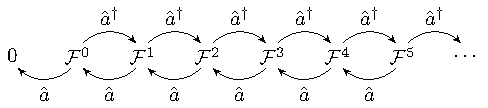
\includegraphics{figures/connected_fock_space_bosons.pdf}}
    \hfil
    \subfigure[]{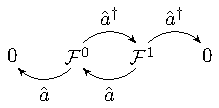
\includegraphics{figures/connected_fock_space_fermions.pdf}}
    \caption{(a) Subspaces $\FS^N$ of $N$-particle bosonic states $\ket{N}$ characterized by a single quantum number. Adjacent spaces are connected through the linear maps $a^{(\dag)}$ defined in \cref{eq:creation,eq:annihilation}. (b) Subspaces for a fermionic system characterized by a single quantum number.}
    \label{fig:fock_spaces}
\end{figure}
Notice the absence of the phase $\nu$ on the right hand side which is due to the fact that the product is ordered.
For this reason, the linear maps $\hat a^\dag_i$ are commonly called creation operators which is what we will call them in the remaining part of this thesis.
Two different linear maps $j<i$ satisfy the following equation
\begin{align}
    \hat a^\dag_i \hat a^\dag_j\ket{n_1,n_2,\dots}_\nu = \nu \hat a^\dag_j\hat a^\dag_i\ket{n_1,n_2,\dots}_\nu,
\end{align}
and thus span the famous (anti-) commutation relation
\begin{align}
    \commutator{\hat a^\dag_i, \hat a^\dag_j}_\nu \coloneqq \hat a^\dag_i \hat a^\dag_j - \nu \hat a^\dag_j \hat a^\dag_i = 0.
\end{align}
From the Hermitian adjoint of the equations before we get the condition
\begin{align}
   \braket{n_1,\dots,n_i,\dots | \hat a^\pdag_i | m_1, \dots, m_i,\dots}_\nu =
   \sqrt{n_i+1}\nu^{\sum_{j<i}n_j} \delta_{n_1,m_1}\dots\delta_{n_i+1,m_i}\dots
\end{align}
and thus
\begin{align}
   \hat a^\pdag_i \ket{n_1, \dots, n_i,\dots}_\nu =
   \sqrt{n_i}\nu^{\sum_{j<i}n_j} \ket{n_1, \dots, n_i-1,\dots}_\nu,
   \label{eq:annihilation}
\end{align}
from which we obtain the algebra relations of the creation/annihilation operators
\begin{align}
    \commutator{\hat a^\pdag_i,\hat a^\dag_j}_\nu = \delta_{i,j},
    \quad
    \commutator{\hat a^\pdag_i,\hat a^\pdag_j}_\nu = 0,
    \quad
    \commutator{\hat a^\dag_i,\hat a^\dag_j}_\nu = 0.
    \label{eq:Heisenberg_algebra}
\end{align}
Proceeding in a reversed manner,~\cref{eq:Fock_basis} is a consequence of the Stone-von Neumann theorem which states that, given the Heisenberg algebra defined through~\cref{eq:Heisenberg_algebra}, the action of the operators and the representation of the Fock basis is unique (up to unitary transformations)~\cite{Hall2013}.

To conclude this first section, a change of basis $\{\ket\alpha\}\rightarrow\{\ket\beta\}$ yields\footnote{Remember that $\mathbb1 = \sum_\alpha\ket{\alpha}\bra{\alpha}$, $\ket{\beta} = \sum_\alpha\ket{\alpha}\braket{\alpha|\beta}$ and $\ket{\beta}=\hat a^\dag_\beta\ket{0}$, leading to \cref{eq:creation_annihilation_basis_rotation}.} a unitary transformation of the operators
\begin{align}
    \hat a^\dag_\beta = \sum_\alpha \braket{\alpha|\beta}\hat a^\dag_\alpha,
    \quad
    \hat a^\pdag_\beta = \sum_\alpha \braket{\beta|\alpha}\hat a^\pdag_\alpha
    \label{eq:creation_annihilation_basis_rotation}
\end{align}
which requires only a computation of the single-particle matrix elements $\braket{\alpha|\beta}$.
Before we move on to the representation of observables, a word on common notations: Quite often the authors assume a certain particle statistics and operator algebra at the beginning of their work which implies a constant (and thus dropped) subscript $\nu$.
In such cases, fermionic annihilation operators are mostly identified through the letter $\hat c$ whereas $\hat b$ often corresponds to bosonic operators.
Furthermore, a common convention identifies the commutator through crotchets
\begin{align}
    \left[\hat A,\hat B\right]\coloneqq\commutator{\hat A,\hat B}_+ = \hat A\hat B - \hat B\hat A
\end{align}
and the anticommutator through curly braces
\begin{align}
    \anticommutator{\hat A,\hat B}\coloneqq\commutator{\hat A,\hat B}_- = \hat A\hat B + \hat B\hat A.
\end{align}
Let me also provide a useful expression to evaluate the commutation relation of operator products recursively
\begin{align}
    \commutator{\hat A, \hat B \hat C}_\pm
    &= \hat A\hat B\hat C \mp \hat B\hat C\hat A + \hat B\hat A\hat C - \hat B\hat A\hat C
    \\
    &= \commutator{\hat A, \hat B}_\pm\hat C \mp \hat B\hat C\hat A \mp \hat B\hat A\hat C
    = \commutator{\hat A, \hat B}_\pm\hat C \mp \hat B\commutator{\hat A,\hat C}.
    \label{eq:recursive_commutation}
\end{align}
In many cases, the sets of quantum numbers are continuous (e.g. position $x$) and as such a sum in \cref{eq:creation_annihilation_basis_rotation} is promoted to an integral expression:
\begin{align}
    \hat a(x) = \sum_\alpha \braket{x | \alpha} \hat a_\alpha,
    \quad
    \hat a_\alpha = \int{\rd x} \braket{\alpha | x} \hat a(x).
\end{align}
This is commonly highlighted through a bracket notation of the continuous quantum number.
%
%
%%%%%%%%%%%%%%%%%%%%%%%%%%%%%%%%%%%%%%%%%%%%%%%
\section{Representation of generic operators}
\label{sec:representation_of_generic_operators}
%%%%%%%%%%%%%%%%%%%%%%%%%%%%%%%%%%%%%%%%%%%%%%%
Let us start with a general operator acting on a single particle of the full $N$-particle state (usually dubbed one-body operator).
Familiar examples are for example the momentum or the position operator $\hat x_i$, $\hat p_i$ acting on the $i$th particle, or compositions of those like single particle potentials $V(\hat x_i)$.
It is thus not surprizing that the general expression of such operators can be given in terms of the particle creation and annihilation operators we introduced in \cref{sec:creation_and_annihilation_operators}.

A one-body operator $\hat o$ diagonal in an arbitrary single-particle basis $\{\alpha\}$ ($\hat o = \sum_\alpha o_{\alpha}\ket{\alpha}\bra{\alpha}$) is trivially extended to the $N$-particle states written in the same basis
\begin{align}
    \hat O_1
    = \sum_{\alpha_i} o_{\alpha_i}\hat a^\dag_{\alpha_i}\hat a^\pdag_{\alpha_i}.
\end{align}
This is most easily understood: one-body operators act on only a single entity of the full set of particles, leaving the others untouched.
In the diagonal basis of $\hat O_1$, the action of $\hat n_{\alpha_i}\coloneqq \hat a^\dag_{\alpha_i}\hat a^\pdag_{\alpha_i}$ just counts the number of particles in the state $\alpha_i$, which is then multiplied with the expectation value of the single-particle operator.
In a more general basis, the one-body operator transforms according to \cref{eq:creation_annihilation_basis_rotation} resulting in
\begin{align}
    \hat O_1 = \sum_{\alpha, \beta}\braket{\alpha | \hat o | \beta} \hat a^\dag_\alpha \hat a^\pdag_\beta = \sum_{\alpha,\beta}o_{\alpha,\beta}\hat a^\dag_\alpha \hat a^\pdag_\beta
    \label{eq:one_body_operator}
\end{align}
It is now straightforward to introduce generic $2$-body operators $\hat O_2$
\begin{align}
    \hat O_2 = \sum_{\alpha,\beta,\gamma,\delta}O_{\alpha,\beta,\gamma,\delta}\hat a^\dag_\alpha \hat a^\dag_\beta \hat a^\pdag_\gamma \hat a^\pdag_\delta
\end{align}
in which the expectation value reads $O_{\alpha,\beta,\gamma,\delta}\coloneqq \braket{\alpha,\beta | \hat o | \gamma,\delta}$.
For example, a generic two-point interaction $\hat V\ket{r_1,\dots,r_N}=1/2\sum_{n\neq m}V(r_n-r_m)\ket{r_1,\dots,r_N}$ in continuous space takes the second quantized form
\begin{align}
    \hat V = \frac12\int{\rd^d r}\int{\rd^d r'}V({\bf r}-{\bf r'})\hat a^\dag({\bf r})\hat a^\dag({\bf r'})\hat a^\pdag({\bf r'})\hat a^\pdag({\bf r}).
    \label{eq:two_point_interaction}
\end{align}
The generalization to generic $M$-body operators is now straightforward
\begin{align}
    \hat O_M = \sum_{\alpha_1,\dots,\alpha_M}\sum_{\beta_1,\dots,\beta_M}O_{\alpha_1,\dots,\alpha_M,\beta_1,\dots,\beta_M}\hat a^\dag_{\alpha_1}\dots \hat a^\dag_{\alpha_M}\hat a^\pdag_{\beta_1}\dots \hat a^\pdag_{\beta_M}.
\end{align}
%
%
%%%%%%%%%%%%%%%%%%%%%%%%%%%%%%%%
\section{Periodic potentials}
\label{sec:periodic_potentials}
%%%%%%%%%%%%%%%%%%%%%%%%%%%%%%%%
To really see when second quantization becomes useful, I go one step back and review basic properties of a single particle moving in a periodic potential which are effectively characterized by a Hamiltonian composed of generic one-body operators of the form of \cref{eq:one_body_operator}.
In particular, the Hamiltonian considered here reads
\begin{align}
    \hat H_0 = \sum_s\int\rd^d r\, \hat a^\dag_s({\bf r})\brlr{\frac{\hat p^2}{2m}+V_{ae}({\bf r})}\hat a_s^\pdag({\bf r})
\end{align}
% and later impose generic two-body interactions
% \begin{align}
%     \hat V_{ee} = \frac12\sum_{s,s'}\int\rd^dr\int\rd^dr'\,V_{ee}({\bf r}-{\bf r'})a^\dag_s({\bf r})a^\dag_{s'}({\bf r'})a^\pdag_{s'}({\bf r}')a^\pdag_{s}({\bf r})
% \end{align}
with operators $\hat a^\pdag_s({\bf r})$ annihilating a particle with flavor $s$ at position $\bf r$.
The local potential $\hat V_{ae}$ is a collection of $N_a$ local potentials
\begin{align}
    V_{ae}({\bf r}) = \sum_{i=1}^{N_a}V_{ae}({\bf R}_i - {\bf r})
\end{align}
and the value of $V_{ae}$ is determined by the relative distance from the position ${\bf R}_i$.
If the creation operators satisfy the anticommutator algebra in real space
\begin{align}
    \anticommutator{\hat a^\pdag_s({\bf r}),\hat a^\dag_{s'}({\bf r'})}=\delta_{s,s'}\delta({\bf r}-{\bf r'}),
\end{align}
the Hamiltonian defines a spinful fermionic system embedded in a crystal lattice (e.g. electrons of traditional solid state setups).
The bare (Bravais) lattice structure in $d$ dimensions is in general spanned by $d$ linearly independent (not necessary mutually perpendicular and normalized) vectors ${\bf x}_i$ and can thus be defined as the set
\begin{align}
    \mathcal{R} = \anticommutator{\sum_{i=1}^d n_i {\bf x}_i,\ n_i\in\mathds Z}.
\end{align}
Additional vectors $\{{\bf b}_i\}$ (sometimes called the basis) are used to define the position of the potential minima relative to the points of the Bravais lattice, such that every position in the primitive cell is given by ${\bf R}_j = \sum_i n_i {\bf x}_i + {\bf b}_j$ with integers $n_i\in\mathds Z$.
The beauty of this approach becomes visible as soon as we define the lattice translation operator
\begin{align}
    \hat T_{\bf n} : \psi_\alpha({\bf r}) \mapsto \psi_\alpha\brlr{{\bf r}+T_{\bf n}},\ T_{\bf n}\coloneqq\sum_i n_i {\bf x}_i={\bf n}\underline{\bf x}
\end{align}
which translates every function from one position to a distance parametrized through the $d$-dimensional vector ${\bf n}\in\mathds Z^d$ and the collection of all lattice vectors $\underline{\bf x}\coloneqq ({\bf x}_1,\dots,{\bf x}_d)^T$.
The local potential $V_{ae}({\bf r})$ is per definition invariant under lattice translations, and the two-body interaction $V_{ee}({\bf r}-{\bf r'})$ is clearly invariant under continuous translations, such that the full Hamiltonian $\hat H$ commutes with the translation operator and we can write the eigenfunctions of $\hat H$ as eigenfunctions of $\hat T_{\bf n}$.
The eigenfunctions of all translation operators $\hat T_{\bf n}$ are called Bloch waves and have the following properties\footnote{Note here that a further restriction on the values of the vector ${\bf k}$ arise from imposing boundary conditions. For instance, Born-von Karman boundary conditions imply a periodicity after $L_j$ unit translations $\psi_\alpha({\bf r}+ L_j{\bf R}_j)=\psi_\alpha({\bf r})$, which confines the allowed values of $k_j$ to integer multiples of $\frac{\bf G_j}{L_j}$ in which $\bf G_j$ is the reciprocal vector of ${\bf R}_j$, i.e. ${\bf G}_j {\bf R}_j = 2\pi/a$.}
\begin{align}
    \hat T_{\bf n}\psi_{\alpha}({\bf r}) &= c_{\bf n}\psi_{\alpha}({\bf r})\\
    c_{{\bf n}_1}c_{{\bf n}_2} &= c_{{\bf n}_1+{\bf n}_2} \Rightarrow c_{\bf n} = \re^{{\bf s}{\bf n}\underline{\bf x}},\ {\bf s}\in\mathds C^d\\
    1=\int_V\rd^dr\,\abs{\psi_{\alpha}({\bf r})}^2 &= \int_V\rd^dr\,\abs{\hat T_{\bf n}\psi_{\alpha}({\bf r})}^2 \Rightarrow 1=\abs{c_{\bf n}}^2 \Rightarrow {\bf s}=\ri{\bf k},\ {\bf k}\in\mathds R^d
\end{align}
It is now possible to phrase Bloch's theorem~\cite{Bloch1929}, which states that the eigenfunctions of a particle moving in periodic potentials assume the simple structure
\begin{align}
    \psi_\alpha({\bf r}) = \psi_{\alpha{\bf k}}({\bf r}) = \re^{\ri{\bf k}{\bf r}}u_{\alpha{\bf k}}({\bf r}).
    \label{eq:bloch_theorem}
\end{align}
Note that we introduced the translation operators eigenvalue argument $\bf k$ in the list of good quantum numbers.
In particular, $\psi$ is a weighted plane wave in which $u$ inherits the lattice periodicity
\begin{align}
    \hat T_{\bf n} u_{\alpha{\bf k}}({\bf r})
    =
    \re^{-\ri{\bf k}\brlr{{\bf r}+{\bf n}\underline{\bf x}}}c_{\bf n}\psi_{\alpha{\bf k}}({\bf r})
    =
    \re^{-\ri{\bf k}{\bf r}}\re^{-\ri{\bf k}{\bf n}\underline{\bf x}}c_{\bf n}\psi_{\alpha{\bf k}}({\bf r})
    =
    u({\bf r}).
\end{align}
The particular expression of the weights obviously depends on the potential, and obtaining general solutions becomes a hard task even for simple problems\footnote{Except maybe the trivial scenario $V_{ae}({\bf r})={\rm const.}$ which implies $u=1$ in \cref{eq:bloch_theorem}.}.
In general, the wave vector $\bf k$ seems to play the same role as the particle momentum $\bf p$ in the Sommerfeld theory of a free particle.
However, this is not true as is clear from the momentum operator being $\hat{\bf p}=-\ri\hbar\nabla$, and as such
\begin{align}
  \hat{\bf p}\psi_{\alpha{\bf k}}({\bf r}) = \hbar{\bf k}\psi_{\alpha{\bf k}} - \ri\hbar\re^{\ri{\bf k}{\bf r}}\nabla u_{\bf k}(\bf r).
\end{align}
The vector ${\bf k}$ is thus dubbed crystal momentum, remembering the fact that $\psi_{\alpha{\bf k}}$ is only an eigenstate of momentum if the potential is constant and thus $\nabla V_{ae}=0$.
Derivation of the effective potential $V_{ae}$ for real materials and analytic solutions of the Bloch weights $u$ are often quite involved and not of particular interest for this thesis (for more details, see~\cite{AshcroftMermin1978,Czycholl2016}).
Moreover, the introduction of tightly bound systems will make clear that a full knowledge of $u$ is not necessary to characterize the spectrum of such systems.

However, to get an idea of the form of the Bloch functions, let us solve the Schrödinger equation of a particle moving along one-dimension in the potential
\begin{align}
    V_{ae}(x) = V_0 \Theta\brlr{b-{\rm mod}_{a}\commutator{x+b}},\ V_0,a,b\in\mathds R_+
    \label{eq:kronig_penney_potential}
\end{align}
such that the nontrivial contours are of size $b$ and displaced by a factor $a$ called the lattice spacing.
This model is called the Kronig-Penney model~\cite{KronigPenney1931} and provides analytic solutions of bound electrons in the limit $b\rightarrow0$ and $V_0\rightarrow\infty$ such that $bV_0=P$, which is depicted in \cref{fig:kronig_penney_potential}.
\begin{figure}
    \centering
    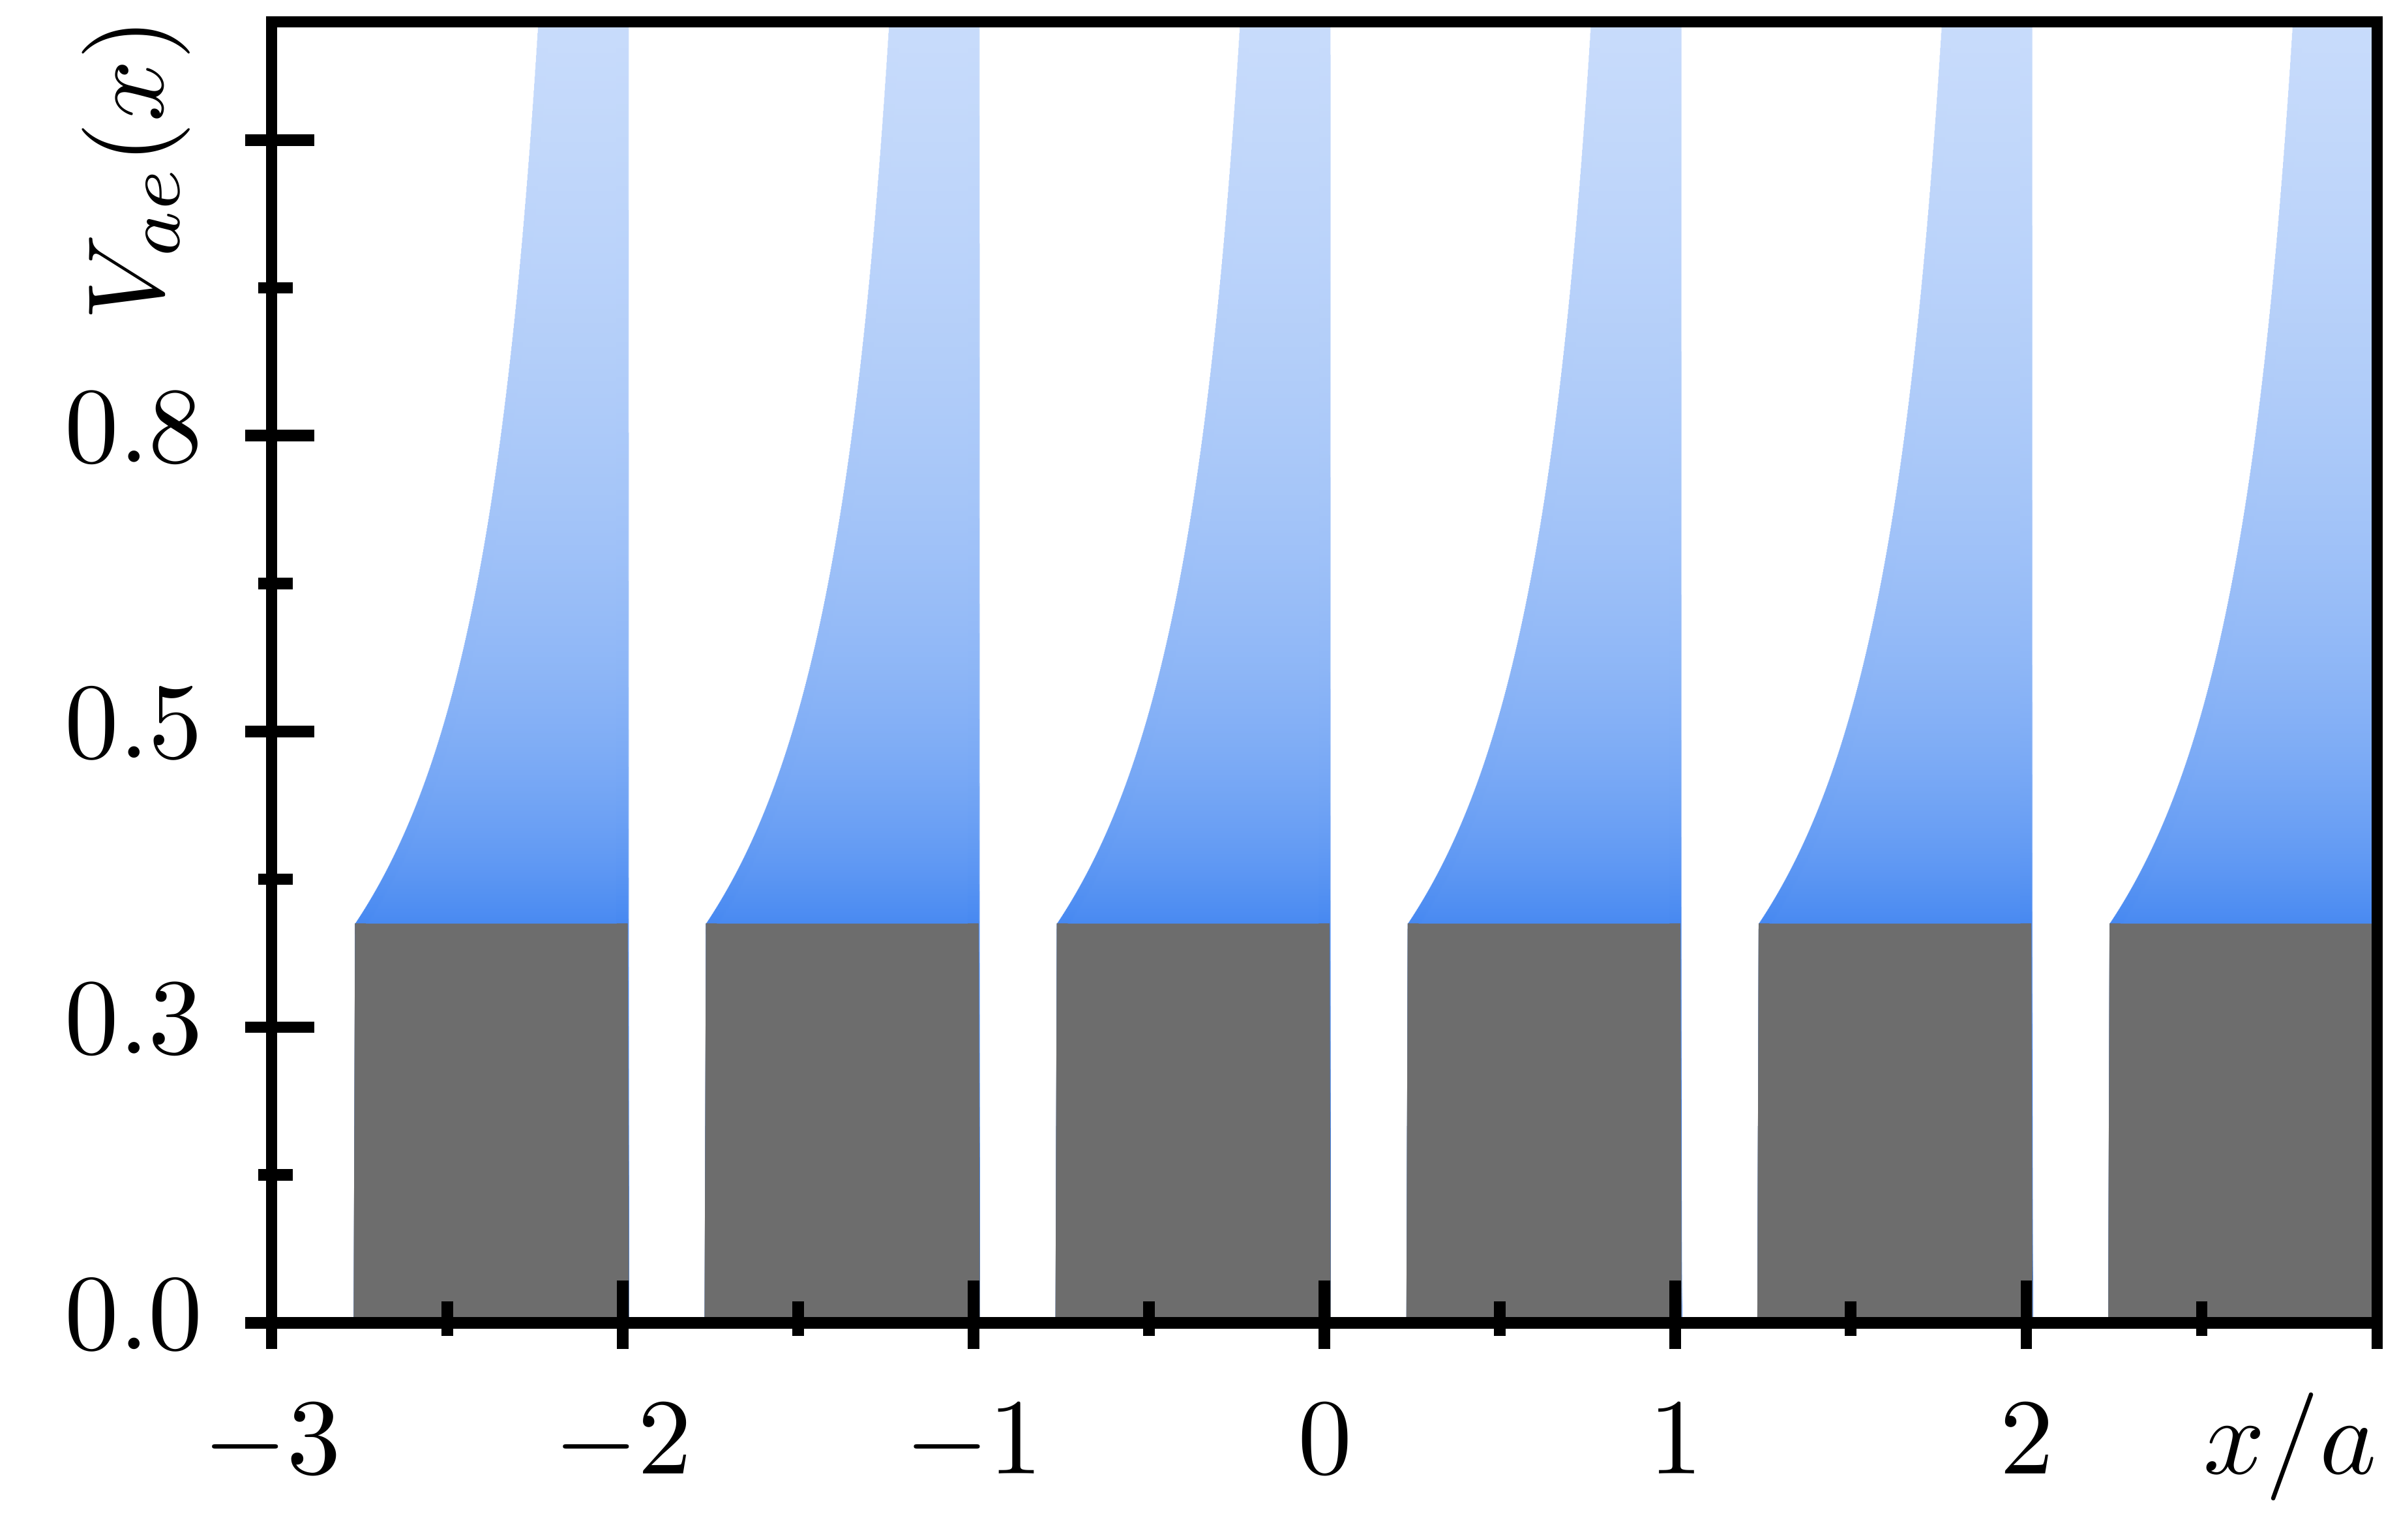
\includegraphics{figures/kronig_penney_potential.png}
    \caption{Contour of the periodic potential \cref{eq:kronig_penney_potential}. The shaded region in blue highlights the limits $b\rightarrow0$ and $V_0\rightarrow\infty$ while preserving a finite product $bV_0=P$ at all times.}
    \label{fig:kronig_penney_potential}
\end{figure}

% In order to preserve the periodicity of the potential, the system size must be commensurate to the lattice spacing $a$, i.e. $L\in a\mathds N$.
To simplify our problem, we can consider it to be a set of two different regions, i.e. (i) a free particle $-\frac{\hbar^2}{2m}\partial_x^2\psi_{\rm (i)}(x) = E\psi_{\rm (i)}(x)$ followed by (ii) a particle moving in a constant potential $-\frac{\hbar^2}{2m}\partial_x^2\psi_{\rm (ii)}(x) = (E-V_0)\psi_{\rm (ii)}(x)$.
In order to read-out the Bloch weights I conveniently factor a crystal momentum from the wave function
\begin{align}
    \psi_{\alpha k}^{\rm (i)}(x) = \re^{\ri kx}u_{\alpha k}^{\rm (i)}(x),
    \
    \psi_{\beta k}^{\rm (ii)}(x) = \re^{\ri kx}u_{\beta k}^{\rm (ii)}(x),
    \\
    u_{\alpha k}^{\rm (i)}(x) = A\re^{(\tau\alpha-\ri k) x} + A'\re^{-(\tau\alpha+\ri k) x},
    \
    u_{\beta k}^{\rm (ii)}(x) = B\re^{(\tau'\beta-\ri k) x} + B'\re^{-(\tau'\beta+\ri k) x},
\end{align}
with $\hbar^2\alpha^2 = 2m\abs{E}$, $\hbar^2\beta^2 = 2m\abs{(E-V_0)}$, $\tau^2=-\sign{E}$ and $\tau'^2=-\sign{E-V_0}$\footnote{Such that plane waves with $\tau=\tau'=\ri$ are obtained for $E>V_0$.}.
The wave functions are supposed to be smooth at the boundaries\footnote{I hereby use the notation of limits from above or below, i.e. $f(0^\pm)=\lim_{\epsilon\rightarrow0}f(\epsilon)$ for $\epsilon>0$.}, which results in
\begin{align}
    % \psi_{\alpha k}^{\rm (i)}(0^+)=\psi_{\beta k}^{\rm (ii)}(0^-),
    % \quad
    % {\psi_{\alpha k}^{\rm (i)}}'(0^+)={\psi_{\beta k}^{\rm (ii)}}'(0^-),
    % \\
    \psi_{\alpha k}^{\rm (i)}(-b+0^-)=\psi_{\beta k}^{\rm (ii)}(-b+0^+),
    \quad
    {\psi_{\alpha k}^{\rm (i)}}'(-b+0^-)={\psi_{\beta k}^{\rm (ii)}}'(-b+0^+),
\end{align}
and the Bloch functions inherit the potential's periodicity
\begin{align}
    u_{\alpha k}^{\rm (i)}(a+0^+) = u_{\alpha k}^{\rm (ii)}(0^-),
    \quad
    u_{\alpha k}^{\rm (i)}{}'(a+0^+) = u_{\alpha k}^{\rm (ii)}{}'(0^-).
\end{align}
In summary, the following matrix equation is derived
\begin{align}
    &\quad M = \nonumber\\
    &\begin{pmatrix}
        1 & 1 & -1 & -1\\
        %
        \tau\alpha & -\tau\alpha & -\tau'\beta & \tau'\beta\\
        %
        \re^{(\tau \alpha-\ri k)(a-b)}  & \re^{-(\tau \alpha+\ri k) (a-b)} &
        -\re^{-(\tau'\beta -\ri k)b}     & -\re^{ (\tau'\beta+\ri k)b} \\
        %
        (\tau \alpha-\ri k)\re^{(\tau \alpha-\ri k)(a-b)}  & -(\tau \alpha+\ri k)\re^{-(\tau \alpha+\ri k) (a-b)} &
        -(\tau'\beta -\ri k)\re^{-(\tau'\beta -\ri k)b}     & (\tau'\beta+\ri k)\re^{ (\tau'\beta+\ri k)b} \\
    \end{pmatrix},
\end{align}
satisfying $M(A,A',B,B')^T=0$.
For nontrivial results, the determinant of $M$ should be equal to zero, which is satisfied for solutions of the transcendental equation
\begin{align}
    \cos(ka)
    =
    \cosh(\alpha\tau(a-b))\cosh(b\beta\tau')
    +
    \frac{\alpha^2\tau^2+\beta^2\tau'^2}{2\alpha\beta\tau\tau'}\sinh(\alpha\tau(a-b))\sinh(b\beta\tau).
    \label{eq:kronig_penney_transcendental_equation}
\end{align}
To approximate the right hand side in the aforementioned limits, application of
\begin{align}
    b\rightarrow0,
    \quad
    V_0\rightarrow\infty,
    \quad
    bV_0 = {\rm constant}
    \\
    \Rightarrow
    b\beta^2\rightarrow 2mbV_0/\hbar^2,
    \quad
    \cosh(b\beta\tau')\rightarrow 1,
    \quad
    \sinh(b\beta\tau')\rightarrow b\beta\tau'
\end{align}
provides an exact solution of \cref{eq:kronig_penney_transcendental_equation} in the limit of narrow and strong periodic potentials\footnote{This limit is actually equivalent to a potential composed by delta-distributions.}
\begin{align}
    f(\alpha a) = \cosh(\alpha\tau a) + \tau'^2\frac{P}{\alpha\tau a}\sinh(\alpha\tau a),
    \quad
    P=mabV_0/\hbar^2.
    \label{eq:kronig_penney_transcendental_equation_approx}
\end{align}
If we assume bound states between the potential wells $0<E<V_0$, the signs become $\tau^2=-1$ and $\tau'^2=+1$, such that \cref{eq:kronig_penney_transcendental_equation_approx} evaluates to
\begin{align}
    f(\alpha a) = \cos(\alpha a) + \frac{P}{\alpha a}\sin(\alpha a).
    \label{eq:kronig_penney_transcendental_equation_approx_bound}
\end{align}
The right-hand-side of \cref{eq:kronig_penney_transcendental_equation_approx_bound} is in general not bound to the interval $[-1,+1]$ spanned by $\cos(ak)$ and establishes values of $\alpha$ (thus, the square-root of the energy $E$) for which no (real) momentum exists (see \cref{fig:kronig_penney_dispersion} (a)).
Such energies are called forbidden and realize a first understanding of band-gaps induced by the nonzero lattice potential $V_0>0$.

If $P=0$, we are left with the energy-momentum relation of free electrons $k=\alpha$ and thus $E_0={\hbar^2k^2}/({2m})$.
If we approach $P\rightarrow\infty$, the allowed energies are formed by the roots of $f$, which are given by the dominating term and yield discretized energies
\begin{align}
    E_{\infty,n_b}=(\hbar n_b\pi)^2/(2ma^2)
    \label{eq:kronig_penney_energy_tb}
\end{align}
spanned by integer numbers ($n_b=1,2,\dots$).
The intermediate regimes $0<P<\infty$ can be solved by numerical evaluation of \cref{eq:kronig_penney_transcendental_equation_approx_bound} and are plotted in \cref{fig:kronig_penney_dispersion} (a).
Straightforward evaluation of $\arccos(f)$ yields the so-called ``reduced zone scheme'' displayed in \cref{fig:kronig_penney_dispersion} (b).

To get an analytic understanding of the wave functions in the above limit, let's focus on the region without potential (i) [remember that one is interested in the limit $b\rightarrow0$]
\begin{align}
    \psi_{\alpha k}^{\rm (i)}(x) = \re^{\ri kx}u_{\alpha k}^{\rm (i)}(x),
    \quad
    u_{\alpha k}^{\rm (i)}(x) = A\re^{\ri(\alpha-k) x} + A'\re^{-\ri(\alpha+k) x},
    \quad
    u_{\alpha k}^{\rm (i)}(x+na)=u_{\alpha k}^{\rm (i)}(x)
    \label{eq:kronig_penney_wavefunctions}
\end{align}
in which the prefactors are related by\footnote{An additional constraint for $AA^*$ is found by requiring normalization of the wave functions, which allows to compute expectation values. However, it is not needed for the purpose of this section and I refer to \cite{KronigPenney1931}.}
\begin{align}
    A' = -A\frac{1-\re^{\ri(\alpha-k)a)}}{1-\re^{-\ri(\alpha+k)a}}.
    \label{eq:kronig_penney_constants}
\end{align}
Starting from \cref{eq:kronig_penney_transcendental_equation_approx_bound}, we see that for any solution $\alpha a$ satisfying $f(\alpha a)=\cos(k a)$ there are an infinite number of symmetric points in momentum space which fulfill the same equation, i.e. (a) $ka + 2n\pi$ and (b) $-ka+2n\pi$.
Close inspection of \cref{eq:kronig_penney_wavefunctions,eq:kronig_penney_constants} reveals that a transformation according to (a) leaves the wave function invariant, while (b) maps it to the solutions of $-ka$, $-\alpha a$.
In other words, (a) is merely a shift by a unit reciprocal vector and (b) flips the direction of the propagating wave, hence establishes a mirror symmetry at the $ka=0$ axis which is a consequence of the system being invariant under time-reversal.
The properties (a) and (b) allow to define the ``unfolding'' of the reduced zone scheme:
without loss of generality, a crystal momentum $n_b\pi\leq ka<(n_b+1)\pi$ can be uniquely connected to an energy value $n_b\pi\leq \alpha a<(n_b+1)\pi$ by introducing a band index $(n_b=0,1,\dots)$.
Here, the limit of free particles ($P=0$) is readily restored, since \cref{eq:kronig_penney_constants} vanishes for $\alpha a = ka$ (except for the special points $ka=n_b\pi$).
At the special points, \cref{eq:kronig_penney_constants} is actually ill defined and evaluates to the two viable solutions $A'=\pm A$, which can be understood from the two non-commuting limits
\begin{align}
    -\lim_{\alpha a \searrow n_b\pi}\frac{1-\re^{\ri(\alpha a-n_b\pi))}}{1-\re^{-\ri(\alpha a+n_b\pi)}}
    =
    -\lim_{\epsilon\searrow0}\frac{1-\re^{+\ri\epsilon}}{1-\re^{-\ri\epsilon}}
    =
    \lim_{\epsilon\searrow0}\re^{+\ri\epsilon}\frac{1-\re^{-\ri\epsilon}}{1-\re^{-\ri\epsilon}}
    =
    +1,
    \\
    -\lim_{k a \searrow n_b\pi}\frac{1-\re^{\ri(n_b\pi - ka))}}{1-\re^{-\ri(n_b\pi+ka)}}
    =
    -\lim_{k a \searrow n_b\pi}\frac{1-\re^{-\ri(n_b\pi + ka))}}{1-\re^{-\ri(n_b\pi+ka)}}
    =
    -1.
\end{align}
The two allowed eigenfunctions are standing waves $\propto \cos(kx),\sin(kx)$.
By reformulating the special points in terms of the particles de Broglie wavelength $\lambda=2\pi/k$, the formation of standing waves can be understood as a residual effect of (constructive) Bragg reflection on a periodic grid structure.
Standing waves are obtained if the particle's de Broglie wavelength and the spacing of the potential satisfy $2a=n_b\lambda$.
\begin{figure}
    \centering
    \subfigure[]{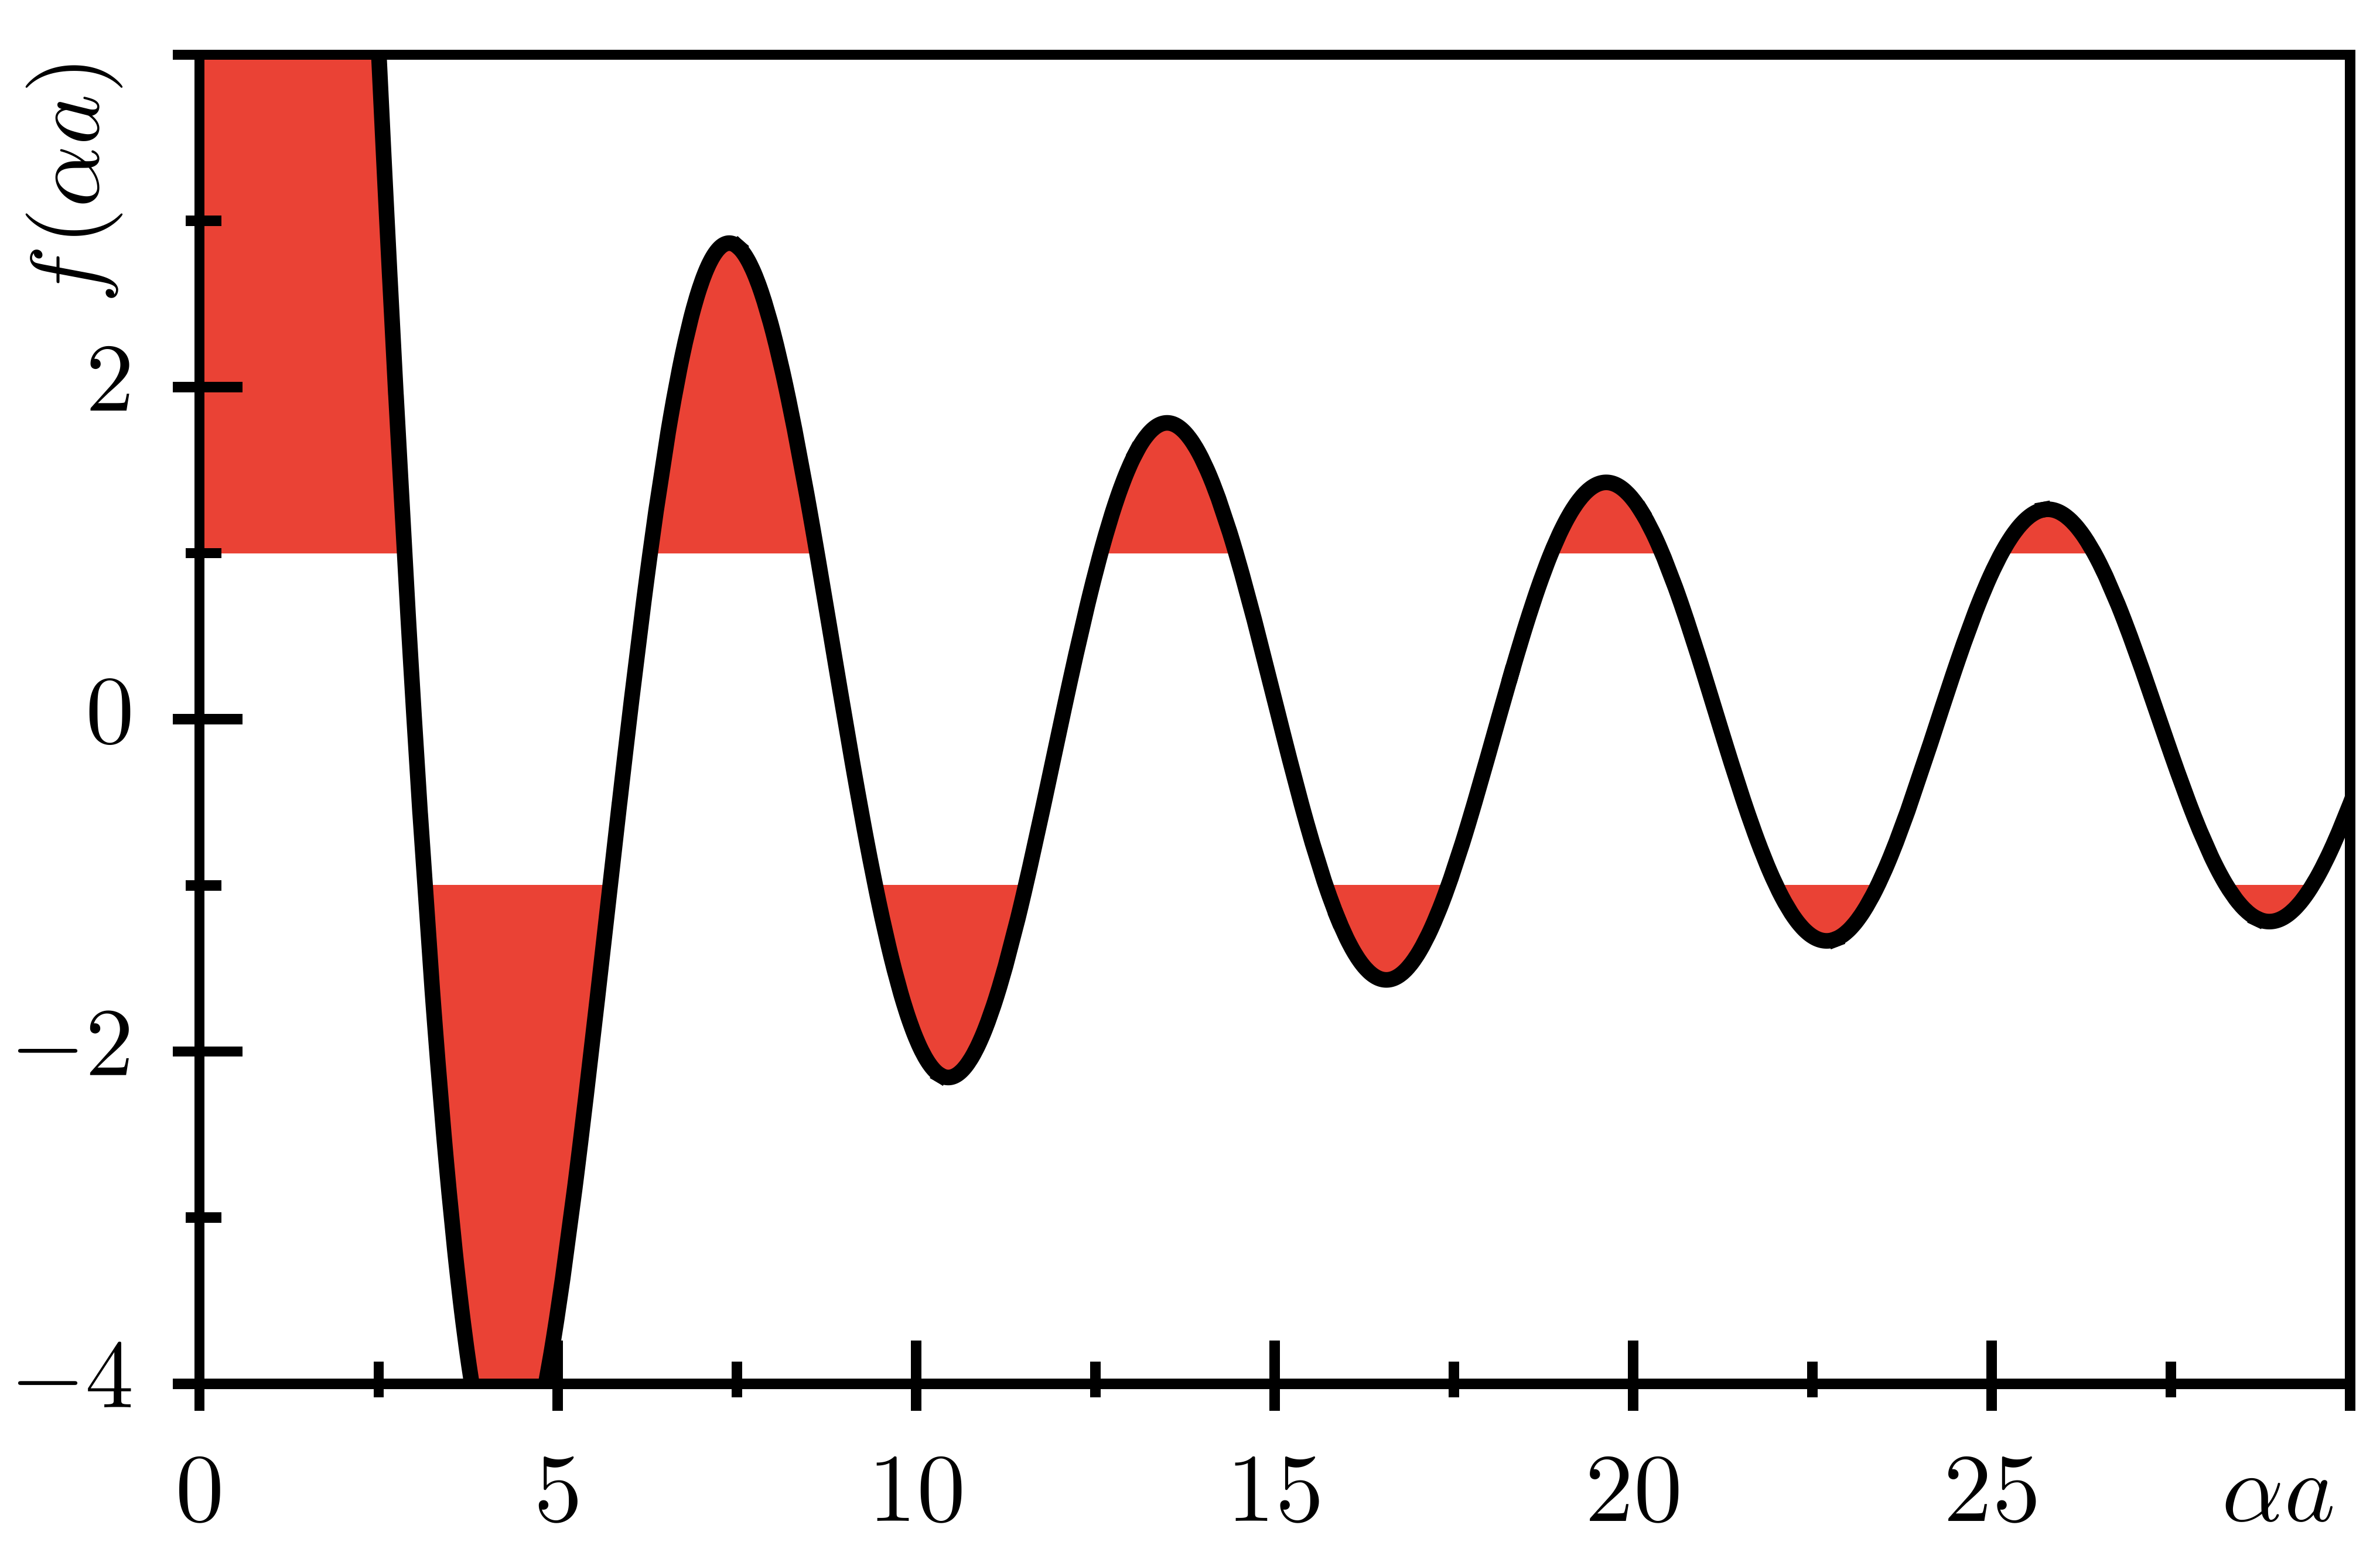
\includegraphics{figures/kronig_penney_transcendental.png}}
    \subfigure[]{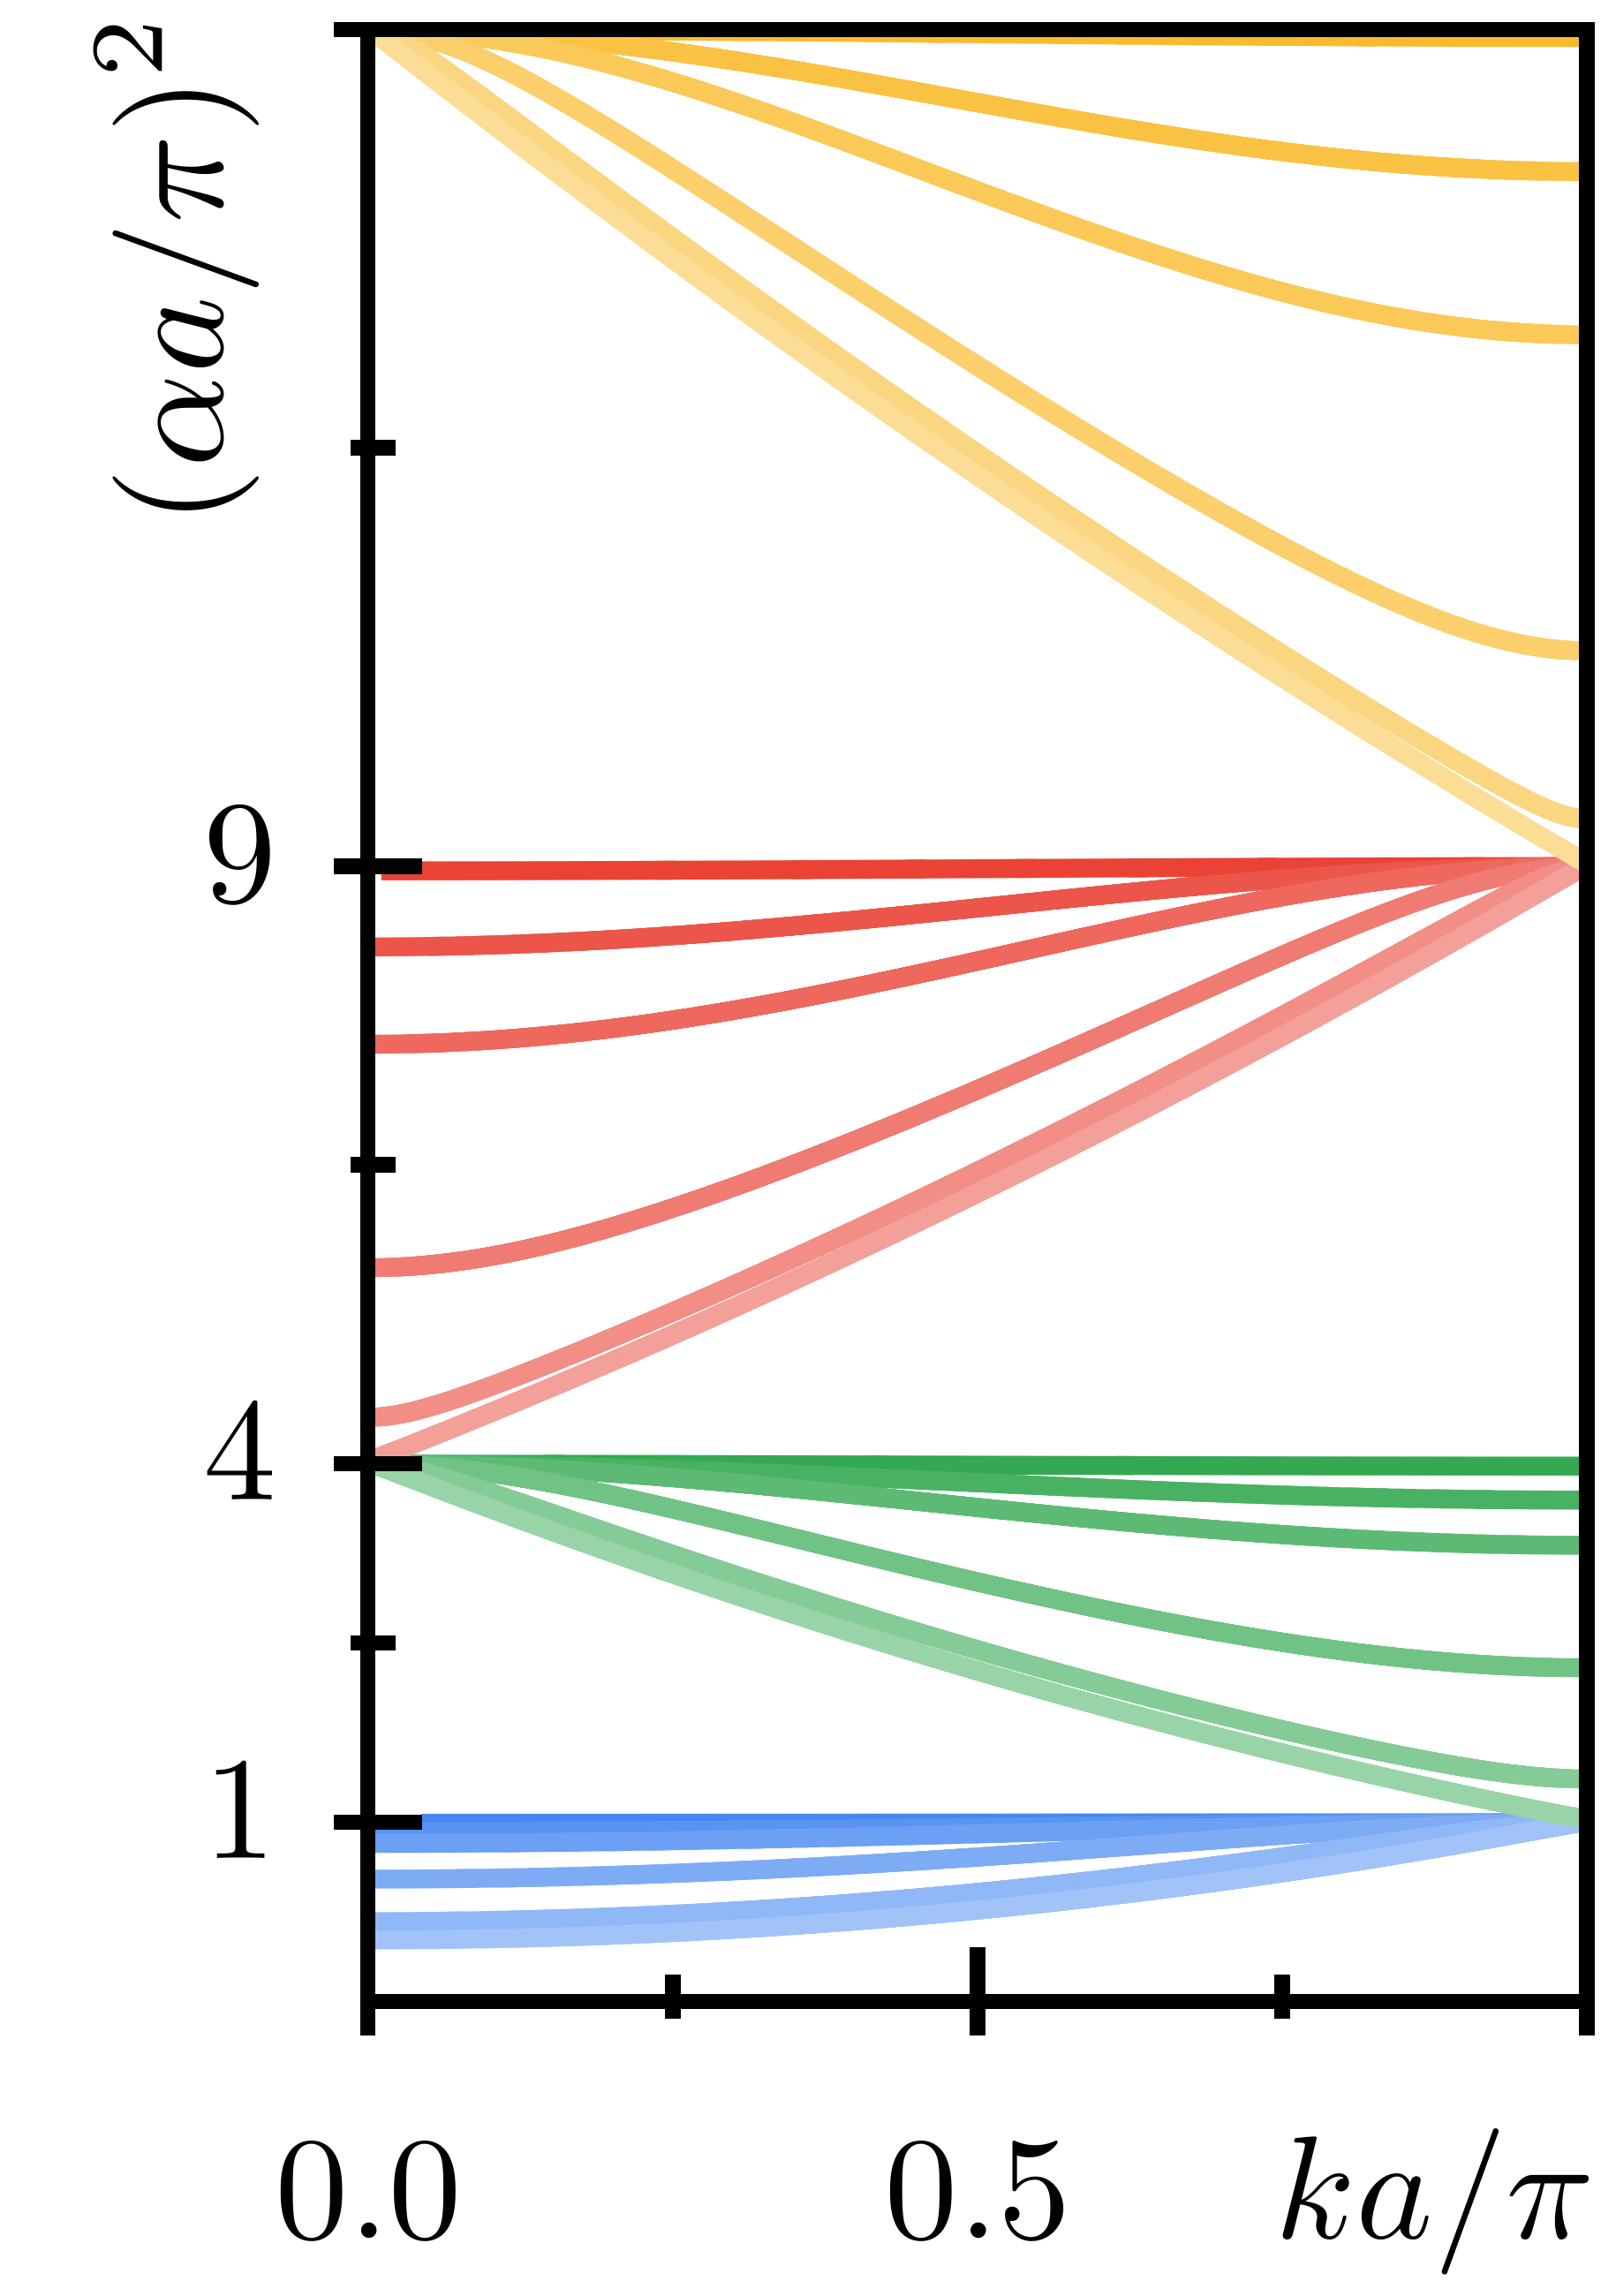
\includegraphics{figures/kronig_penney_dispersion_2.png}}
    \subfigure[]{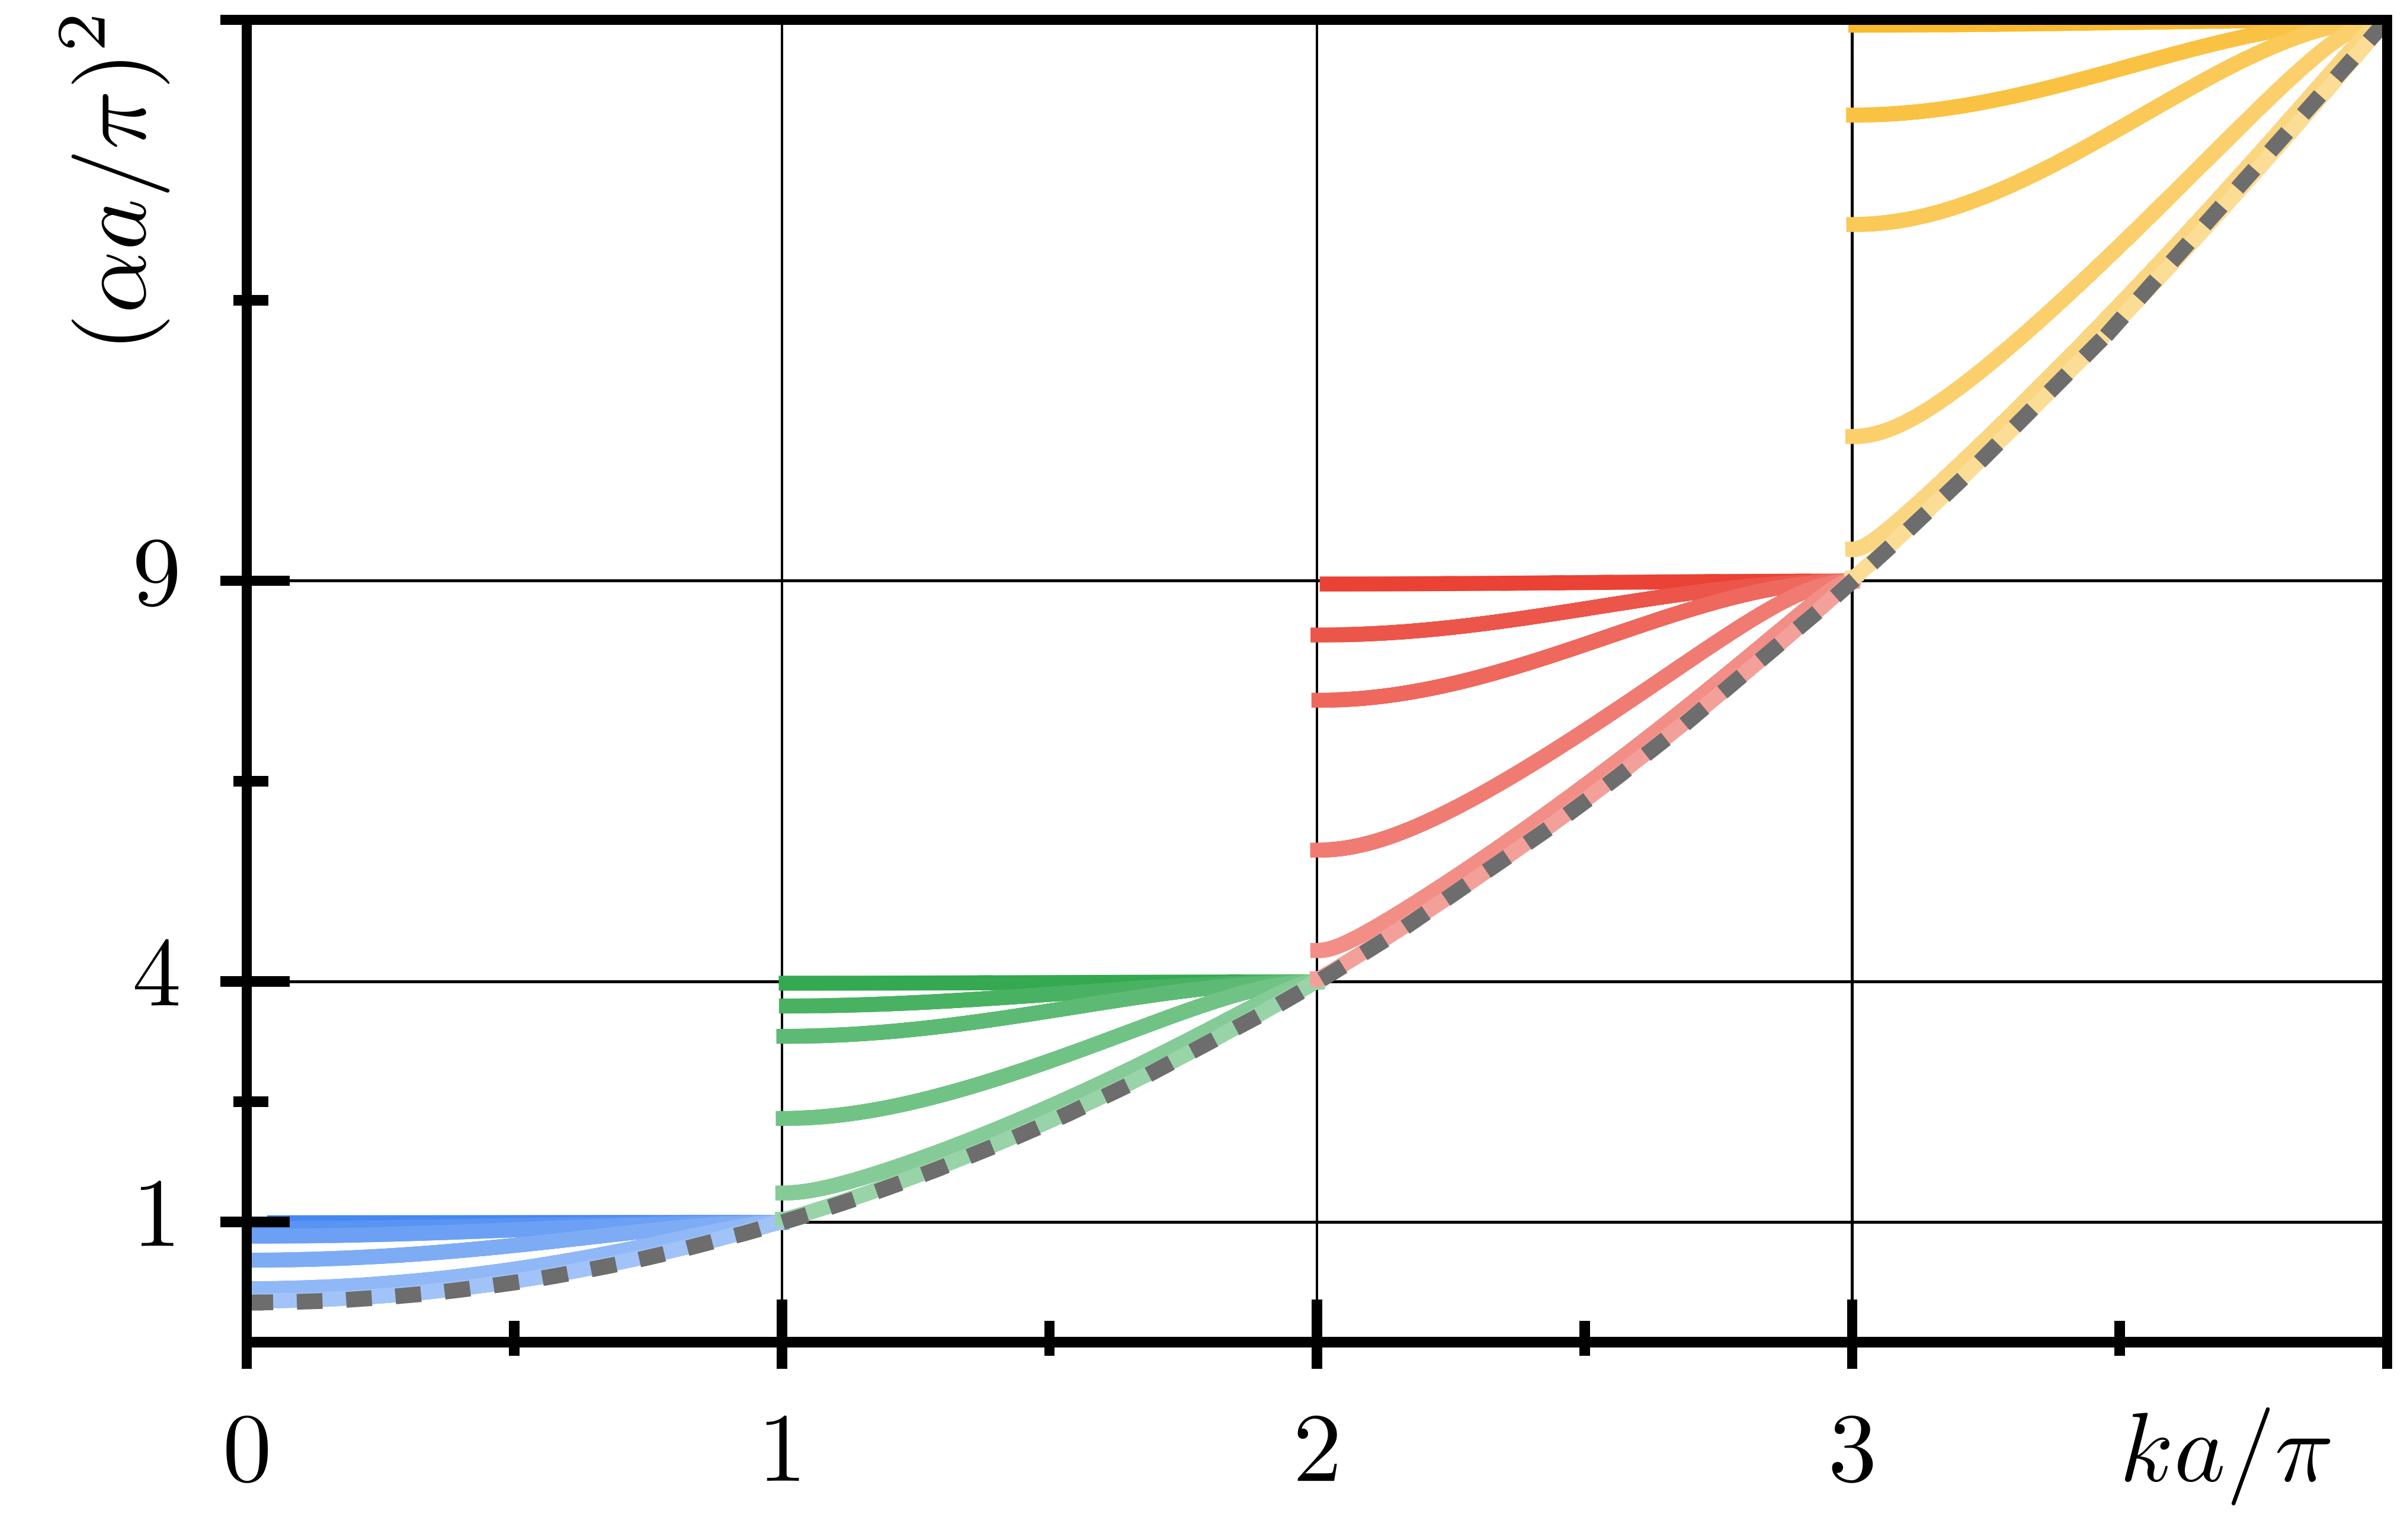
\includegraphics{figures/kronig_penney_dispersion_1.png}}
    \caption{
    (a) Plot of the right-hand-side of the transcendental equation. Solutions do not exist in the red regions.
    (b)-(c) Shapes of the dispersion relation $(\alpha a/\pi)^2$ versus crystal momentum $ka/\pi$ given by \cref{eq:kronig_penney_transcendental_equation_approx_bound}.
    Different opacity (transparent to colors) represent increasing values of $P\in\{0.1,1,5,20,50,1000\}$.
    (c) The properties of the wave functions allow to uniquely relate the crystal momentum $ka$ to an energy $\alpha a$ in which the limit of free electrons [i.e. $P\rightarrow0$] is pronounced.}
    \label{fig:kronig_penney_dispersion}
\end{figure}

In the limit $P\rightarrow\infty$, the energy $E_{\infty,n_b}$ assumes the discrete values in \cref{eq:kronig_penney_energy_tb} resulting in motionless eigenstates -- the resulting waves are tightly bound to the potential minimum.
If we relax this limit a bit, i.e. $P\gg 1$, a reasonable approximation of the lowest band curvature is obtained by a first order Taylor series of \cref{eq:kronig_penney_transcendental_equation_approx_bound} resulting in the typical dispersion relation for tight binding systems, i.e.
\begin{align}
    E_{P\gg1,1}\approx t_0 + t_1 \cos(k a),
    \quad
    t_0 = + E_{\infty,1} - \frac{\pi^2 \hbar^4}{a^3 m^2 b V_0},
    \quad
    t_1 = -\frac{\pi^2\hbar^4}{a^3 m^2 bV_0}.
    \label{eq:kronig_penney_tight_binding_dispersion}
\end{align}

A way to numerically solve generic potentials is obtained by expanding the Schrödinger equation in reciprocal space through the following identities\footnote{The reciprocal space provides a way to Fourier-transform as the functions $\re^{\ri {\bf G r}}$ form a basis on the primitive cell of the real lattice over the square-integrable functions. In particular, the functions satisfy the orthogonality equation $\delta_{\bf G, G'}=\frac1{\Omega}\int\rd^dr\,\re^{\ri({\bf G-G'}){\bf r}}$.}
\begin{align}
    V_{ae}({\bf r}) = \sum_{\bf G}V_{ae}{}_{\bf G}\re^{\ri {\bf G r}},
    \quad
    V_{ae}{}_{\bf G} = \frac1{V}\int\rd^dr\,V_{ae}({\bf r}){\bf G}\re^{-\ri {\bf G r}},
    \\
    u_{n{\bf k}}({\bf r}) = \sum_{\bf G}u_{n{\bf k}}({\bf r}){}_{\bf G}\re^{\ri {\bf G r}},
    \quad
    u_{n{\bf k}}({\bf r}){}_{\bf G} = \frac1{V}\int\rd^dr\,u_{n{\bf k}}({\bf r})\re^{-\ri {\bf G r}},
\end{align}
in which $V$ is the volume of the primitive unit cell.
Straightforward evaluation yields the algebraic eigenvalue problem for the unknown functions $u_{n{\bf k}}{}_{\bf G}$
\begin{align}
    \frac{\hbar^2}{2m}({\bf G}+{\bf k})^2u_{n{\bf k}}{}_{\bf G}+\sum_{\bf G'}V_{ae}{}_{\bf G-G'}u_{n{\bf k}}{}_{\bf G'} = E_{n{\bf k}}.
    \label{eq:periodic_lattices_numerics}
\end{align}
The dimension of the linear equation is infinite due to the sum over all reciprocal lattice vectors and has to be truncated if one wants to solve the equation numerically [the convergence of such a truncation has to be carefully checked for a serious investigation].
Clearly, strongly confined potentials such as delta functions are particularly bad candidates to solve numerically through evaluation of \cref{eq:periodic_lattices_numerics} because the resulting matrix equation will not be sparse and any truncation will result in a significant error.
%
%
%%%%%%%%%%%%%%%%%%%%%%%%%%%%%%%%%%
\section{Tight binding systems}
\label{sec:tight_binding_systems}
%%%%%%%%%%%%%%%%%%%%%%%%%%%%%%%%%%
%
%
The systems considered here are those of tightly bound constituents to the lattice centers.
Such types can be found in traditional solid state scenarios where the nuclei are well separated beyond the typical Bohr radius of the valence electrons, in setups of ultracold atoms trapped in optical lattices, in optical waveguides or polaritons.
In all our works, we cover theoretical aspects of interacting tight binding models which can be experimentally realized in a variety of different setups.
For this reason, it will be useful to review briefly how these models are motivated from first principles, and how they can be understood in the more modern approach of second quantization.

\begin{figure}
    \centering
    \subfigure[]{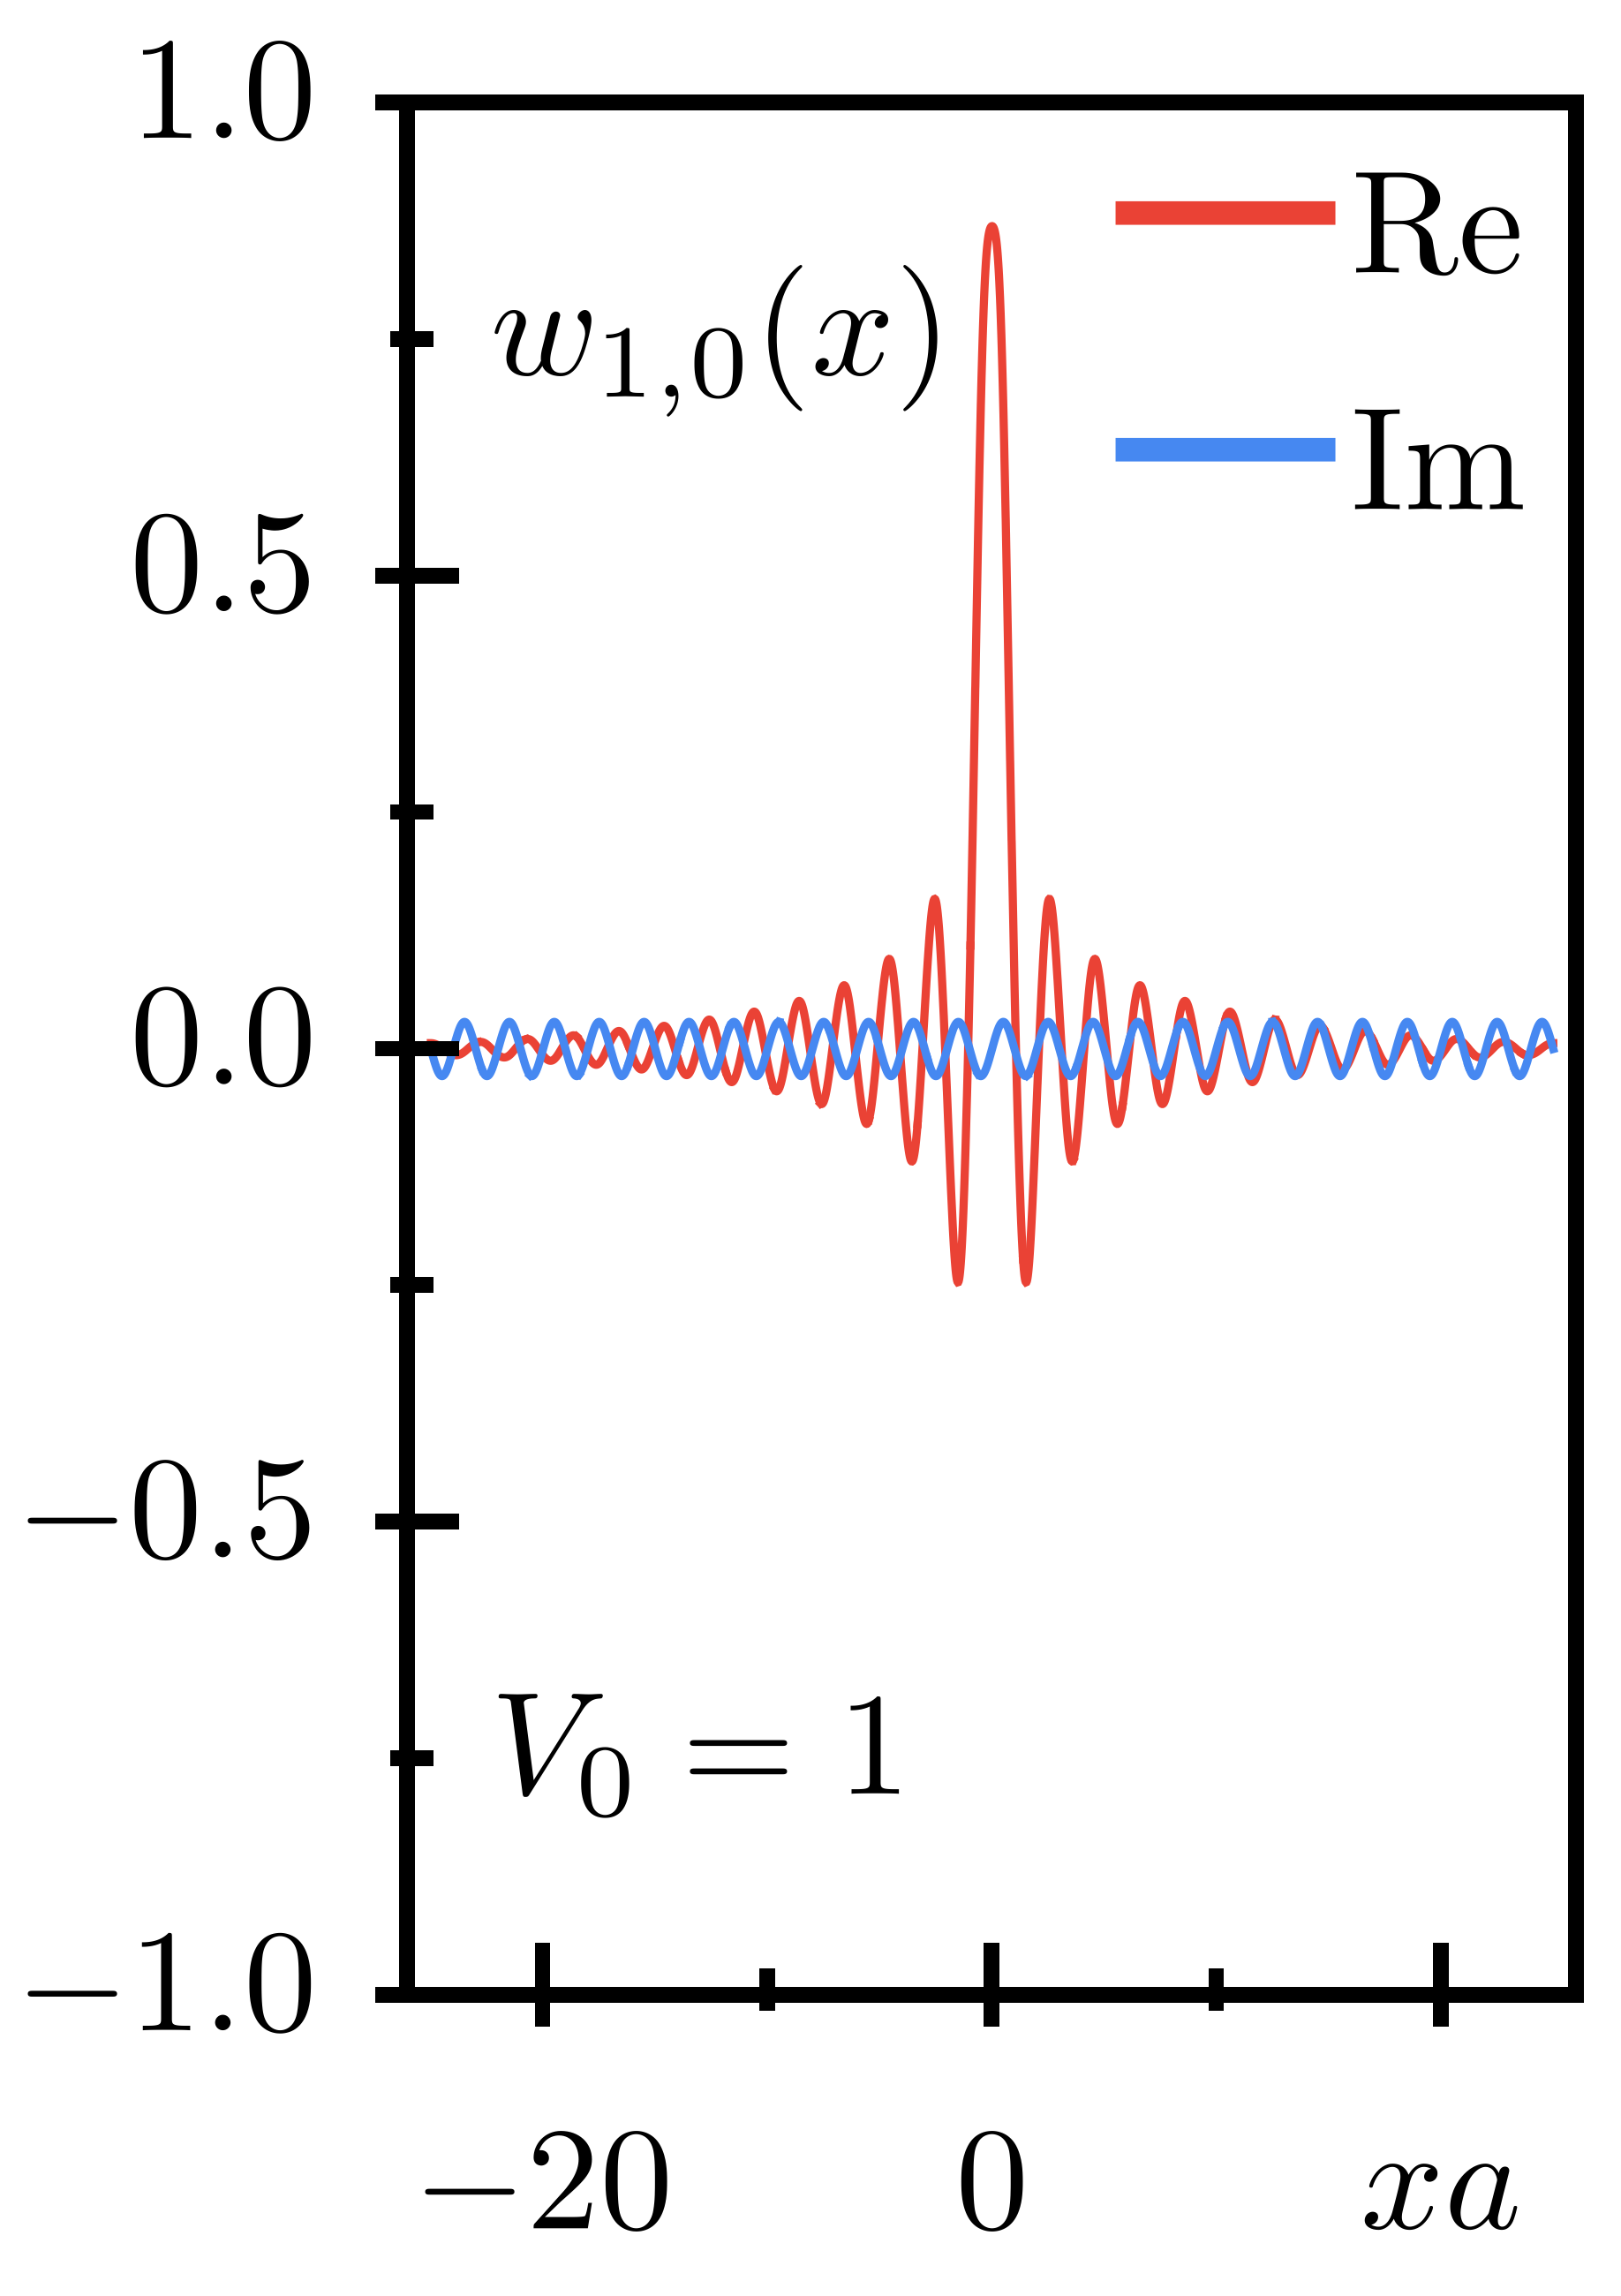
\includegraphics{figures/wannier1_1.png}}
    \subfigure[]{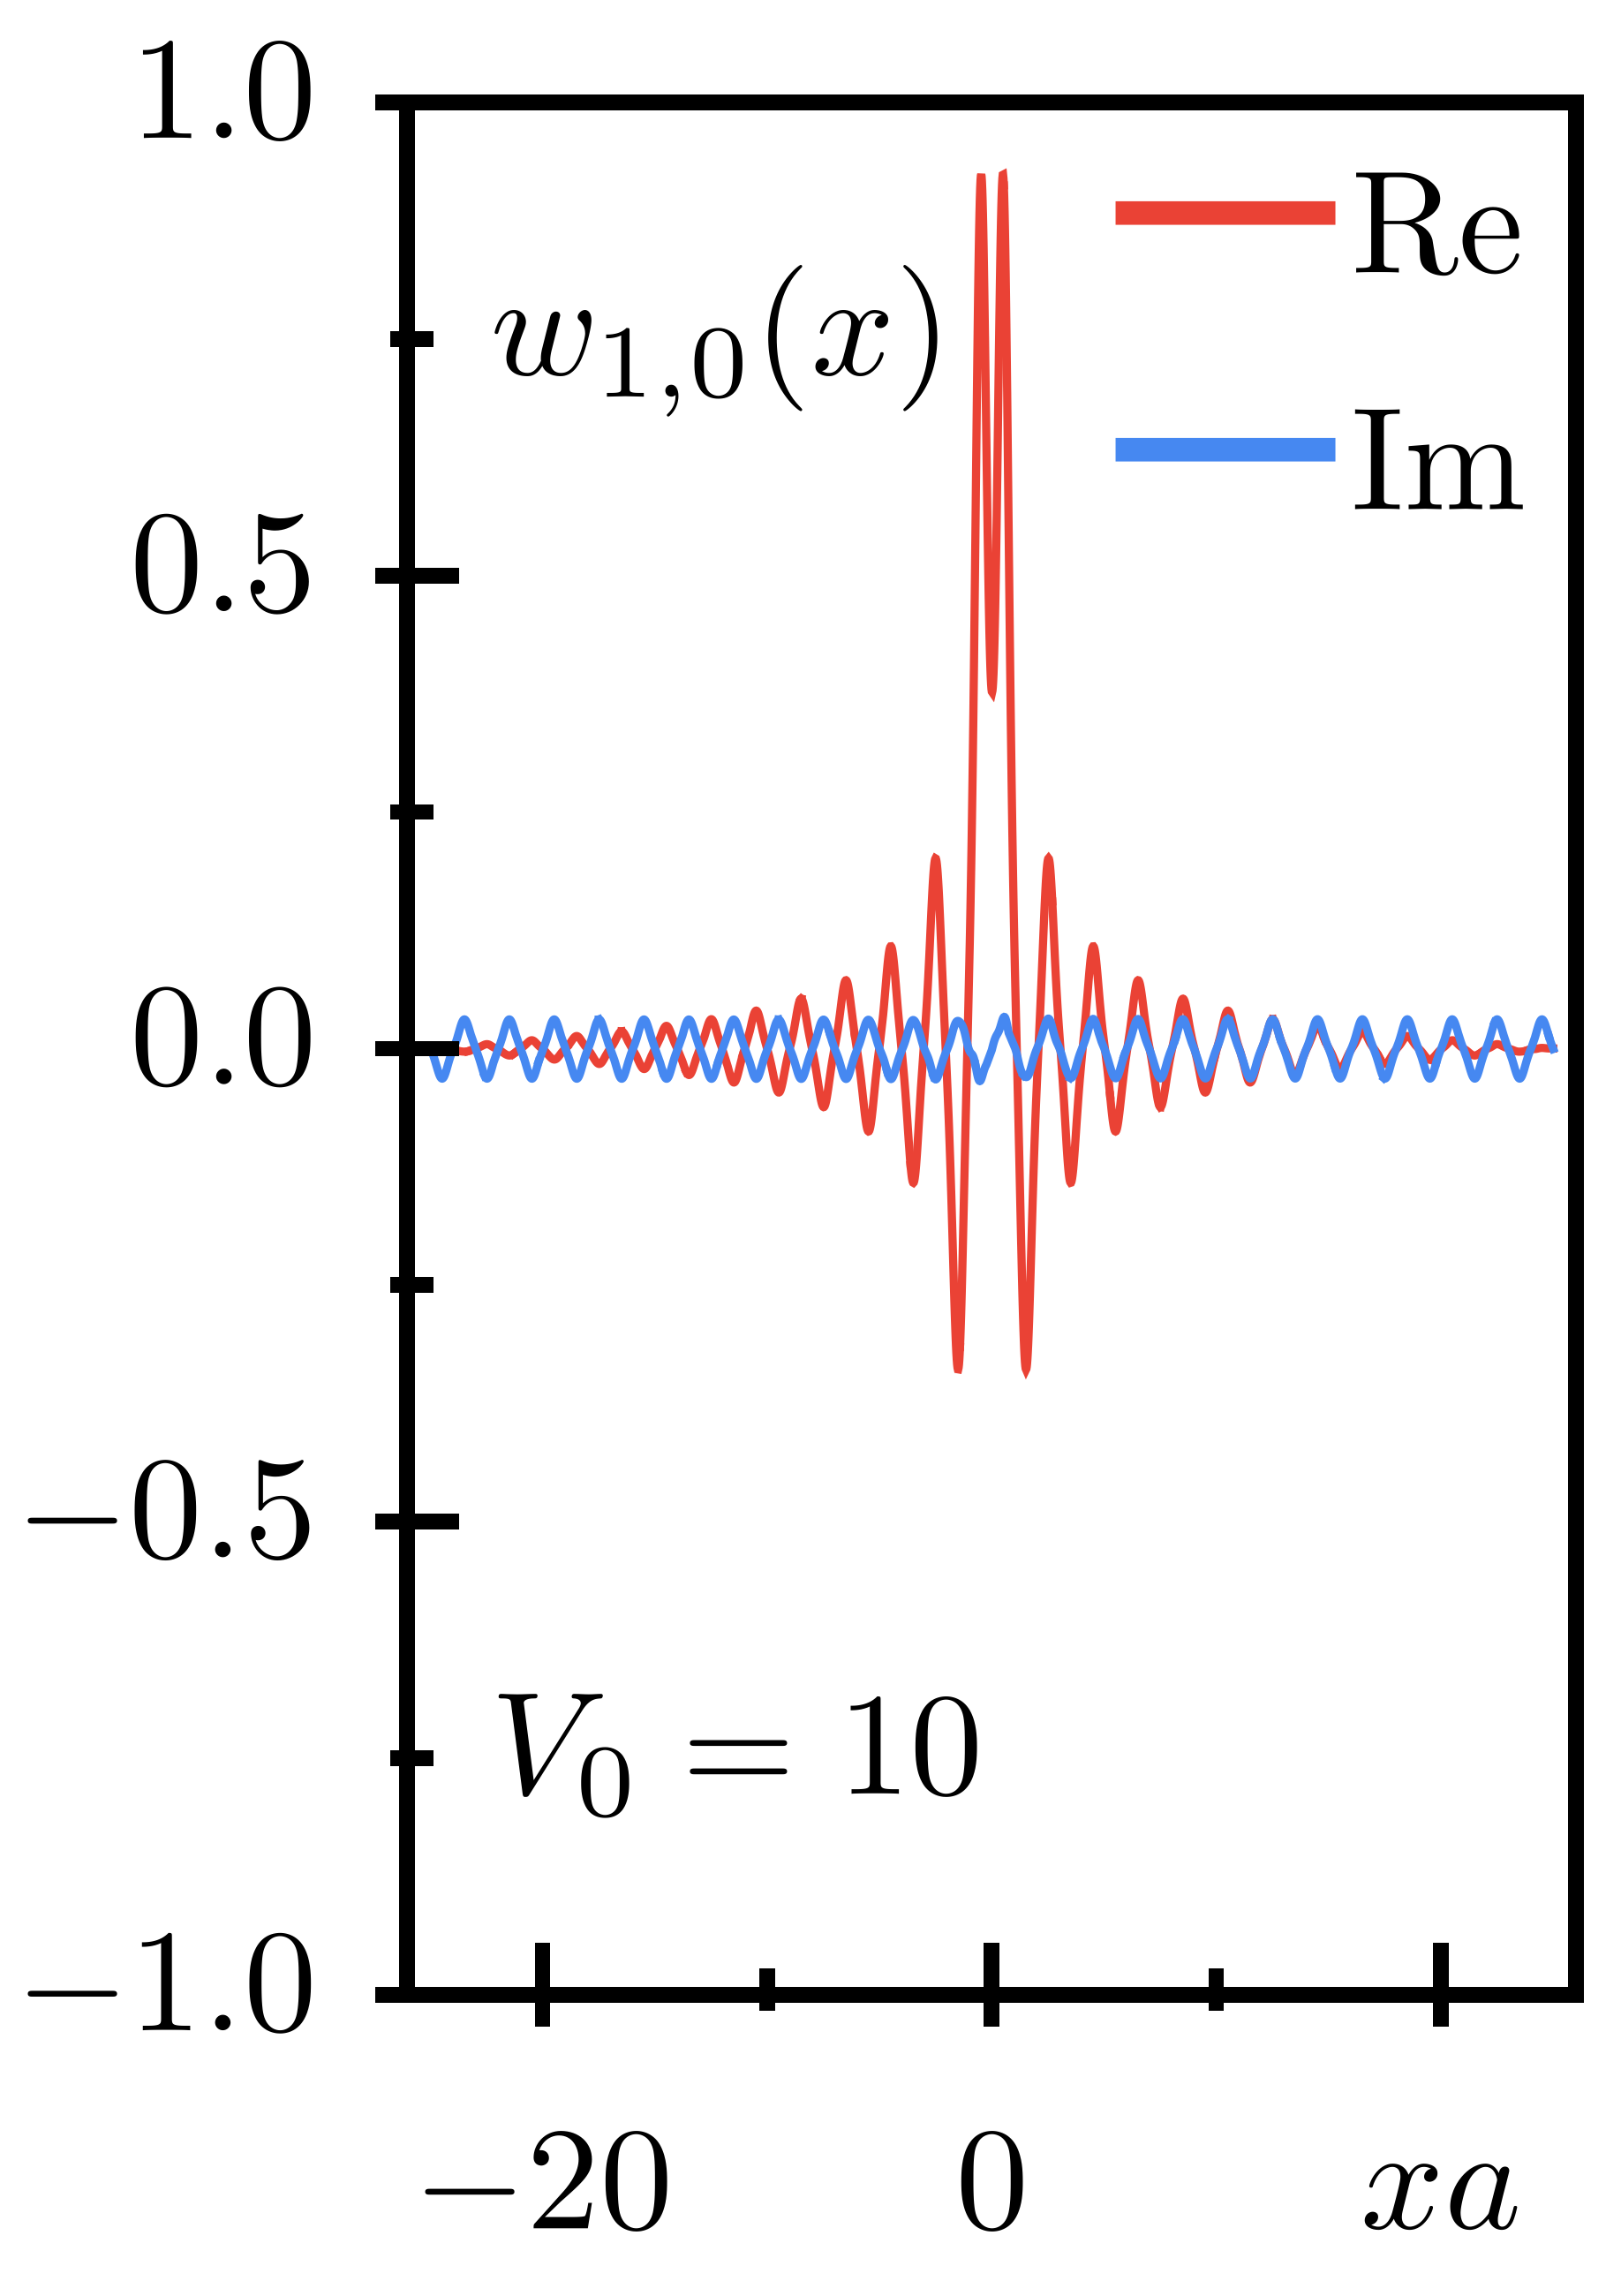
\includegraphics{figures/wannier1_10.png}}
    \subfigure[]{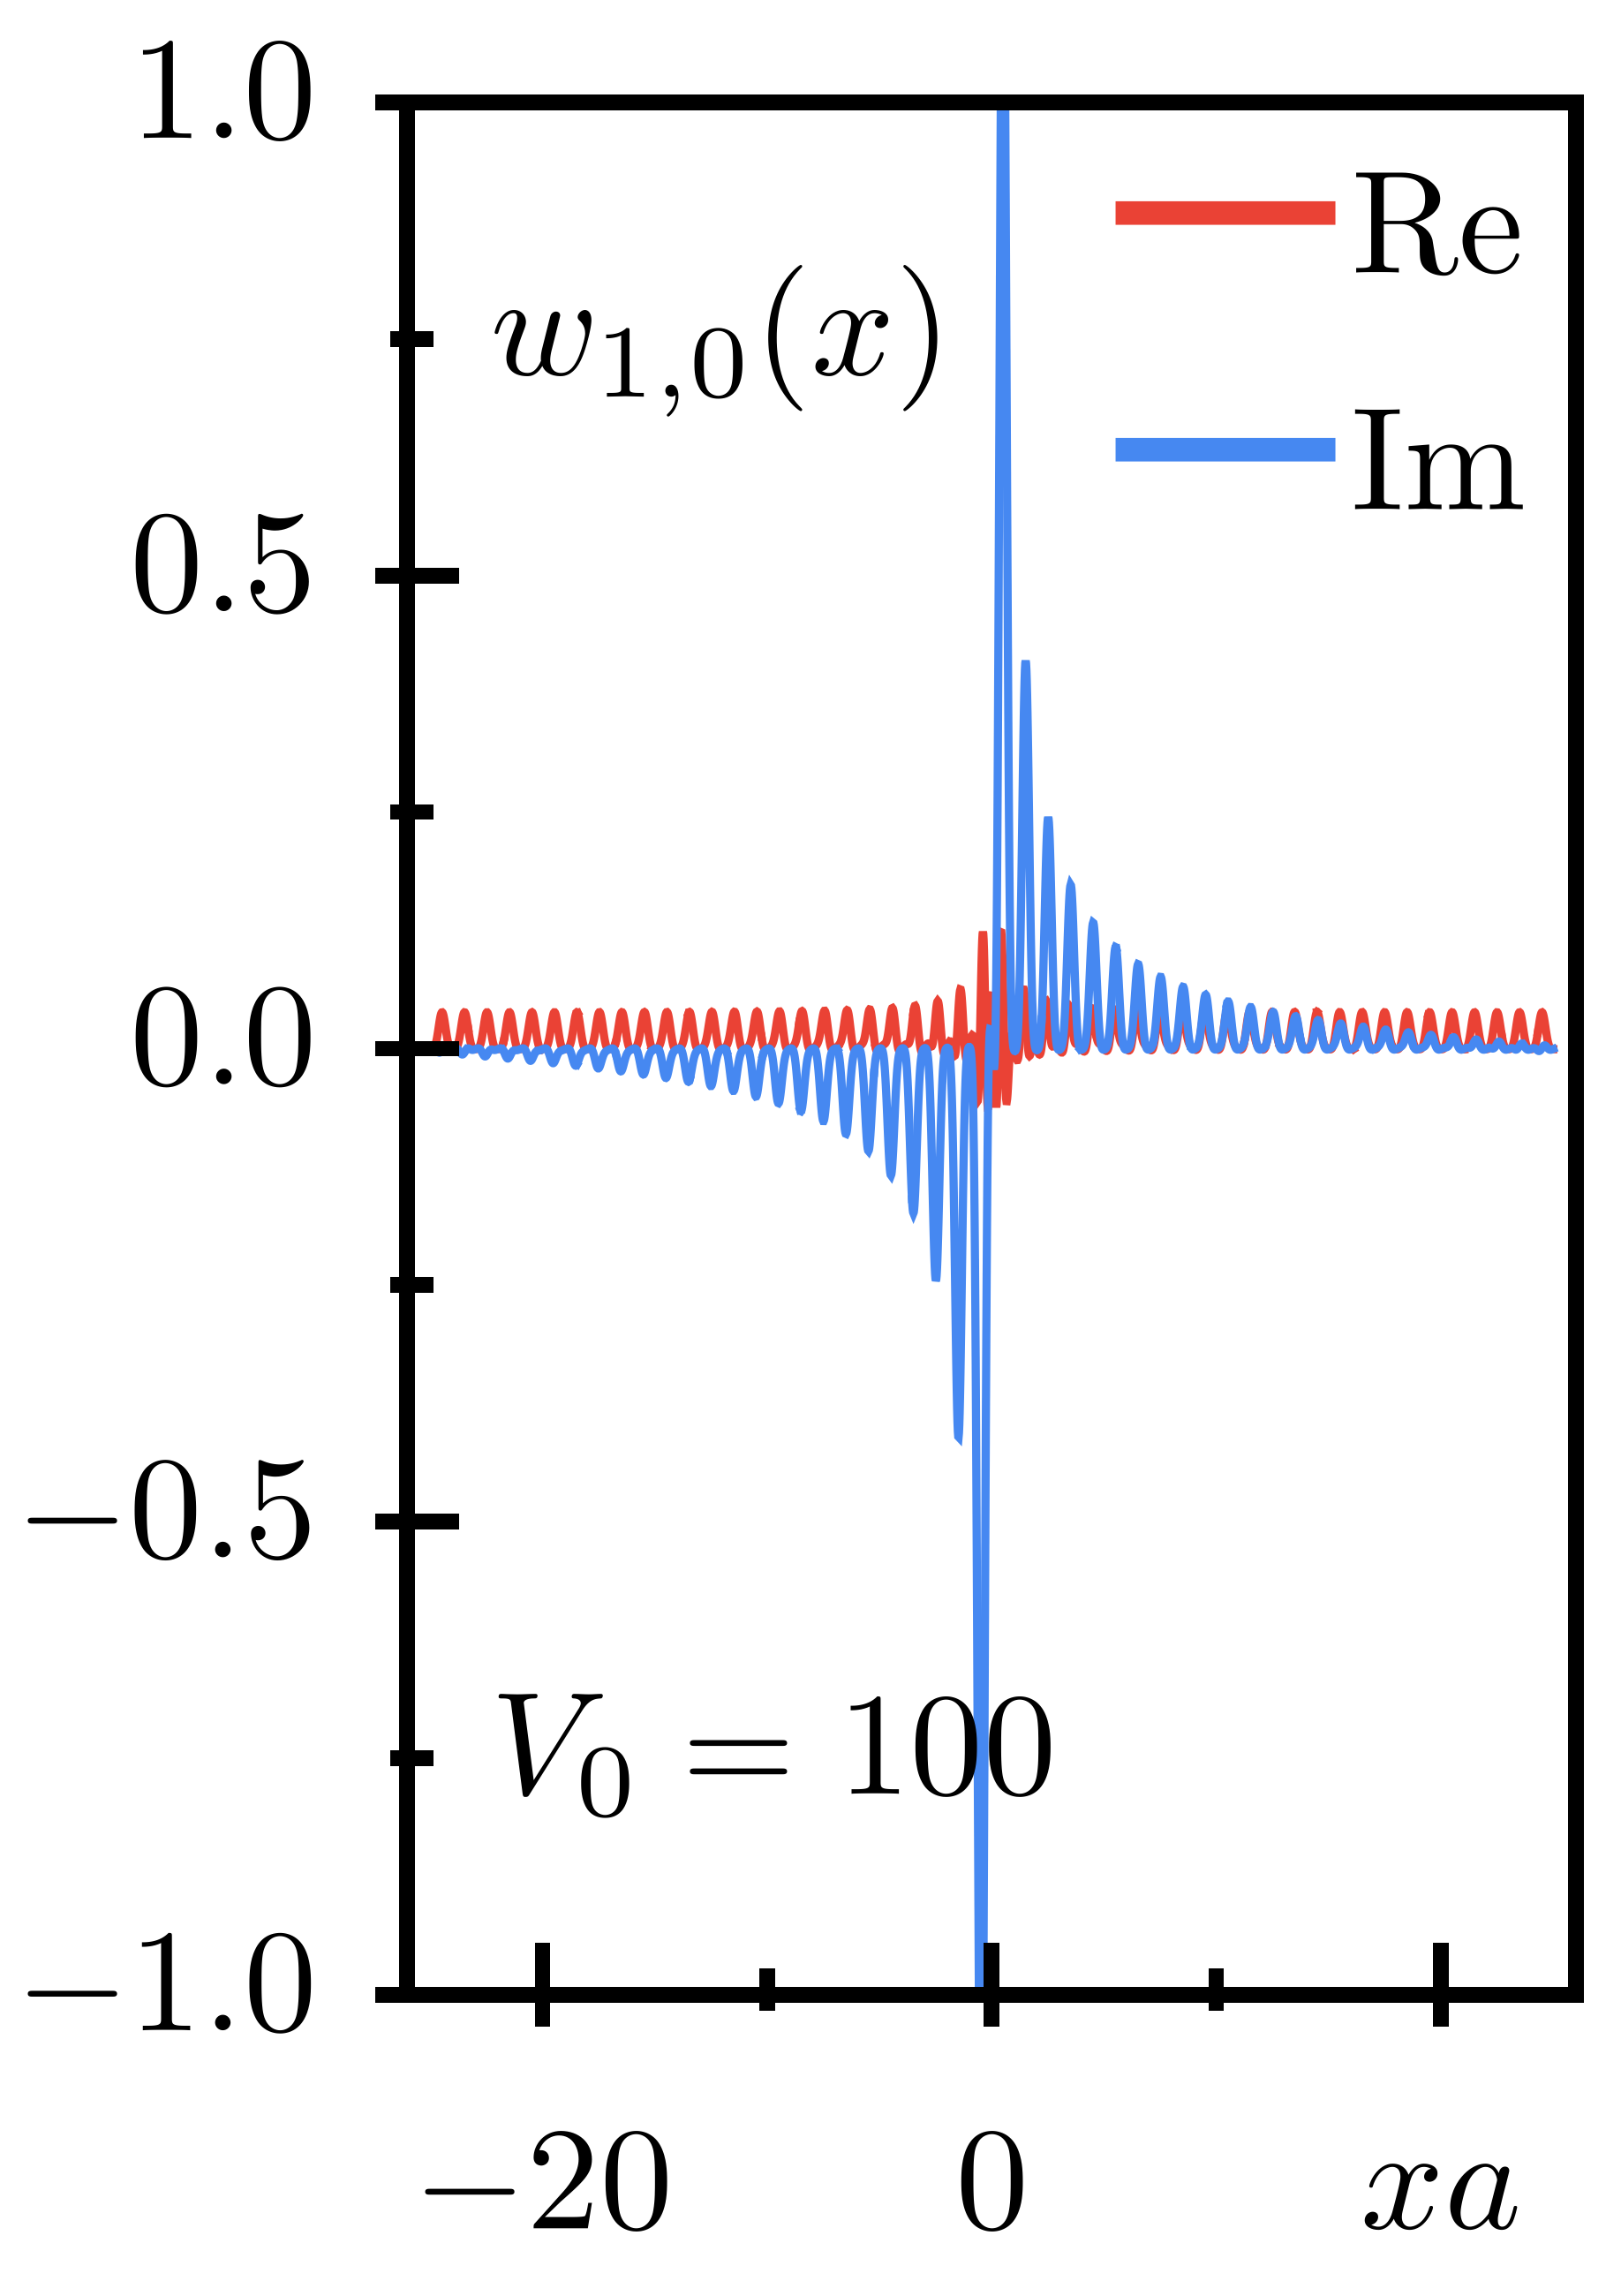
\includegraphics{figures/wannier1_100.png}}\\
    \subfigure[]{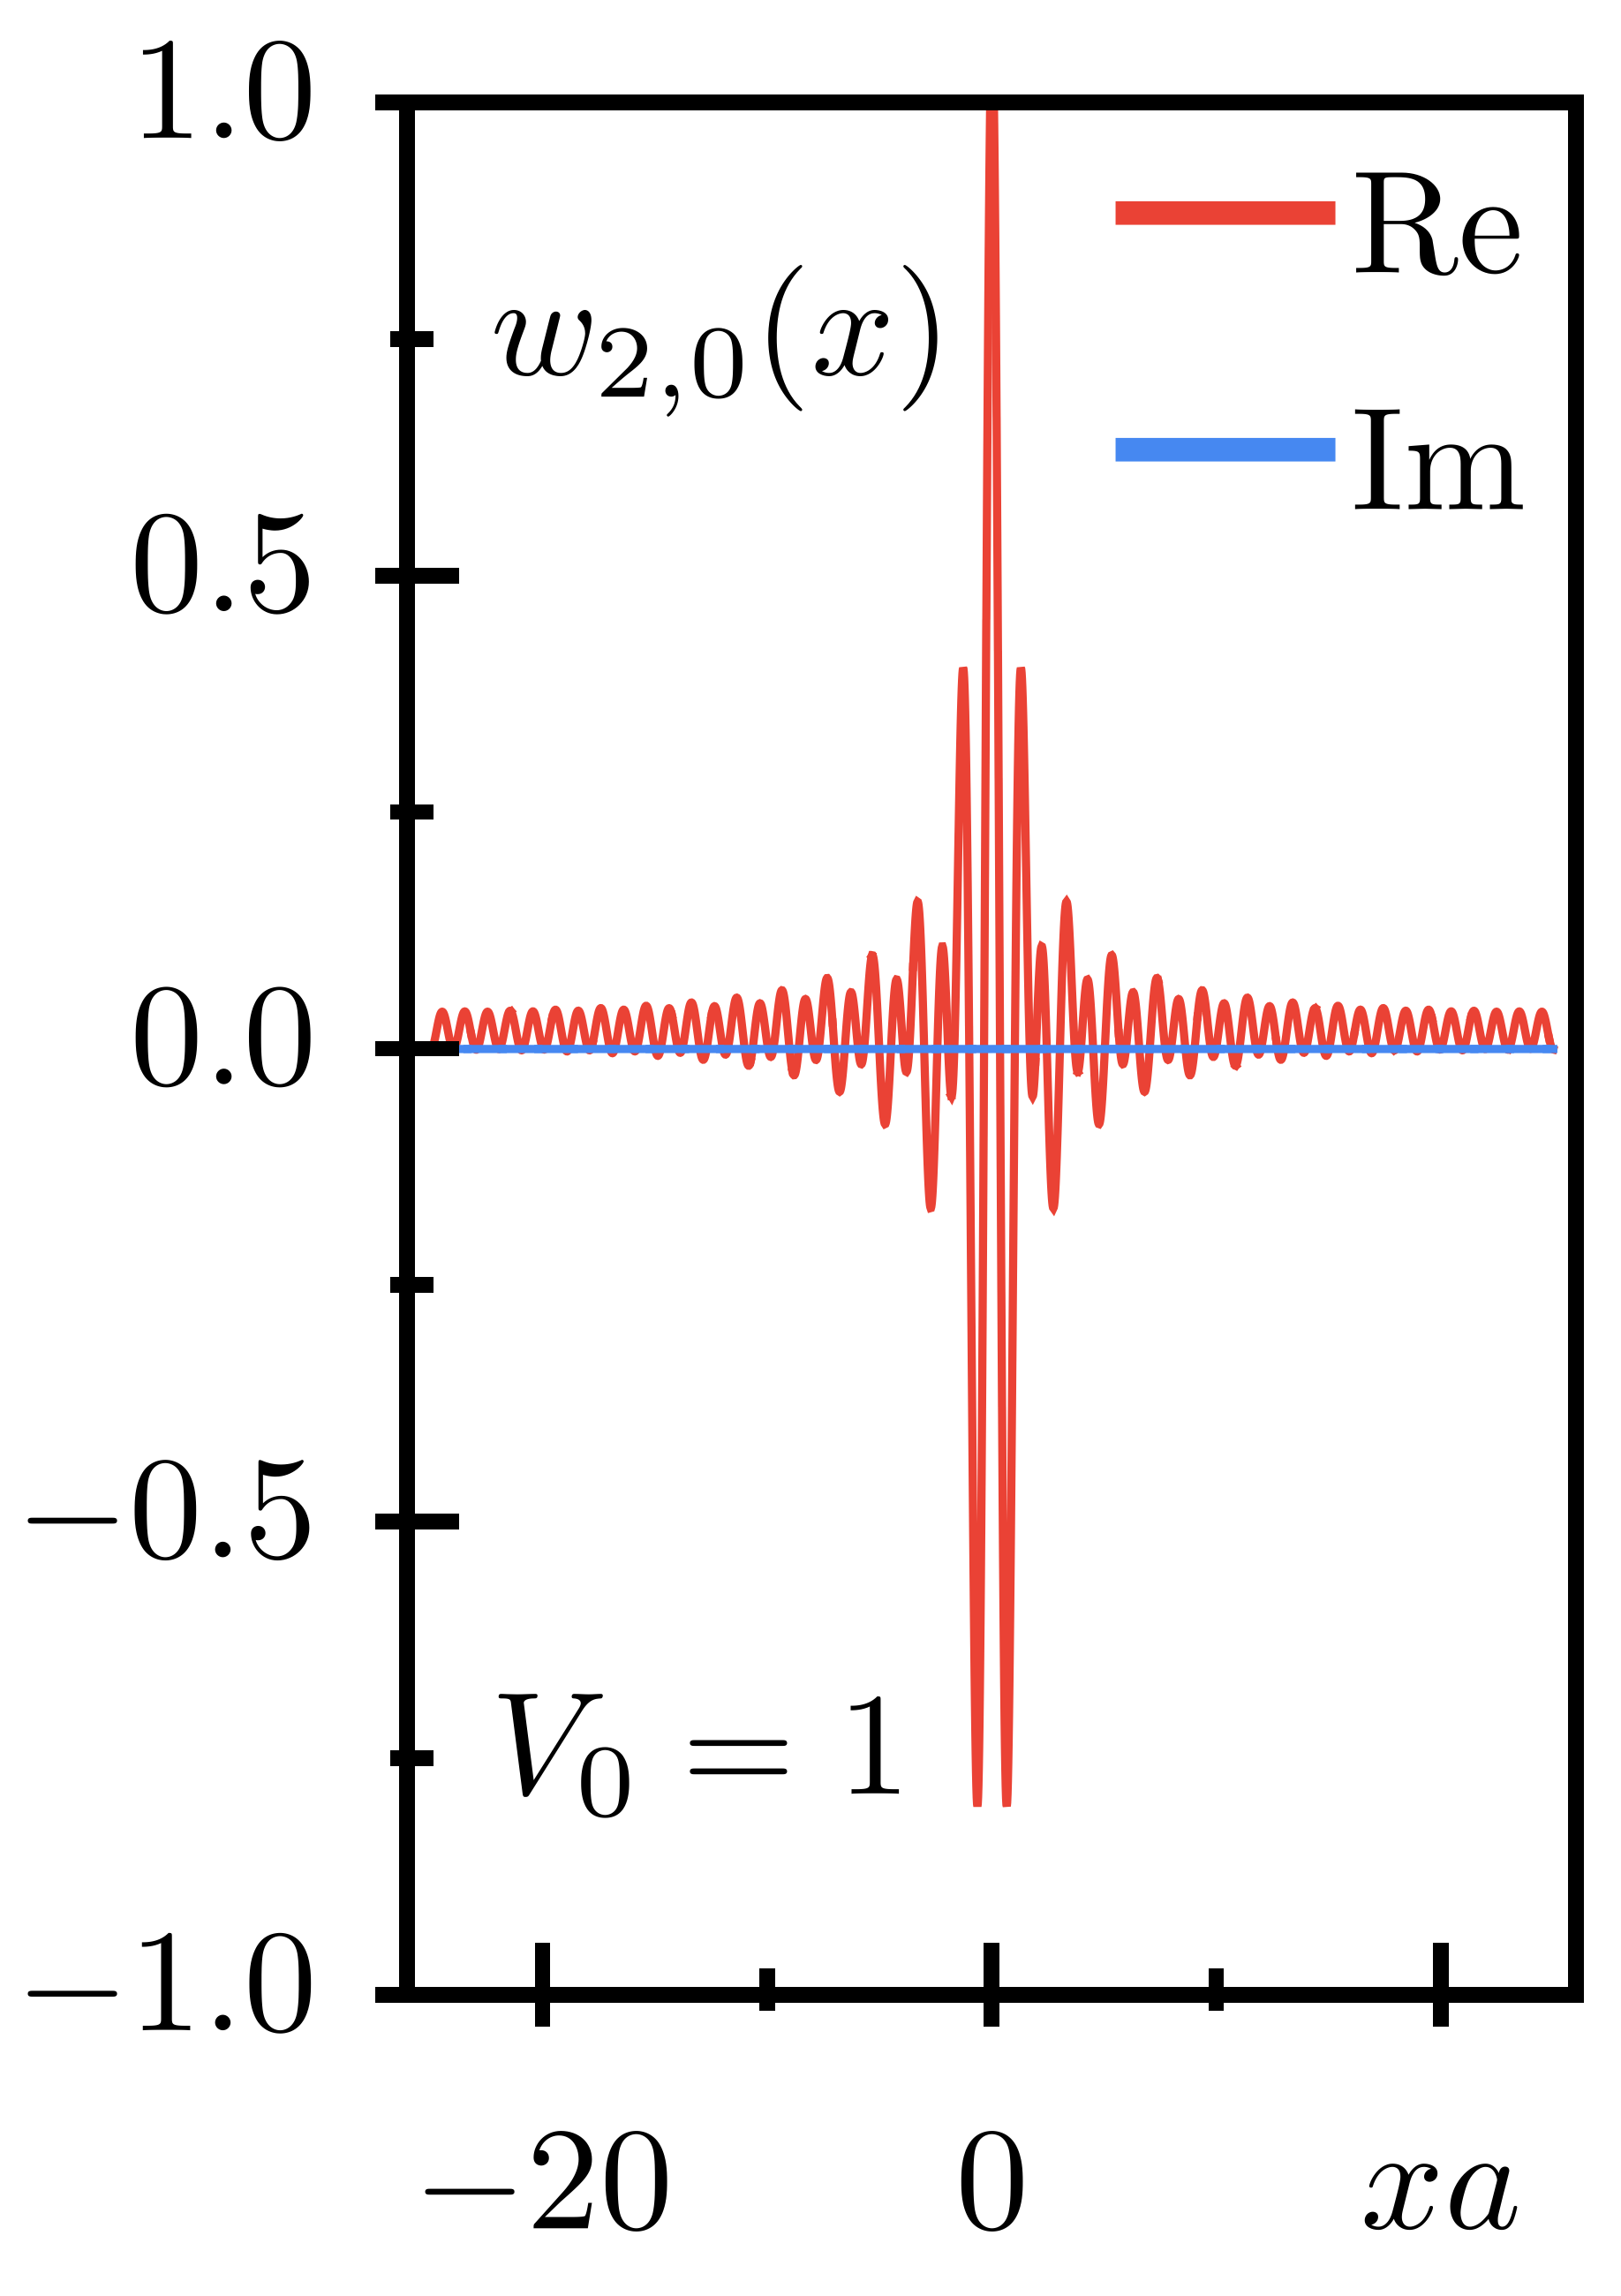
\includegraphics{figures/wannier2_1.png}}
    \subfigure[]{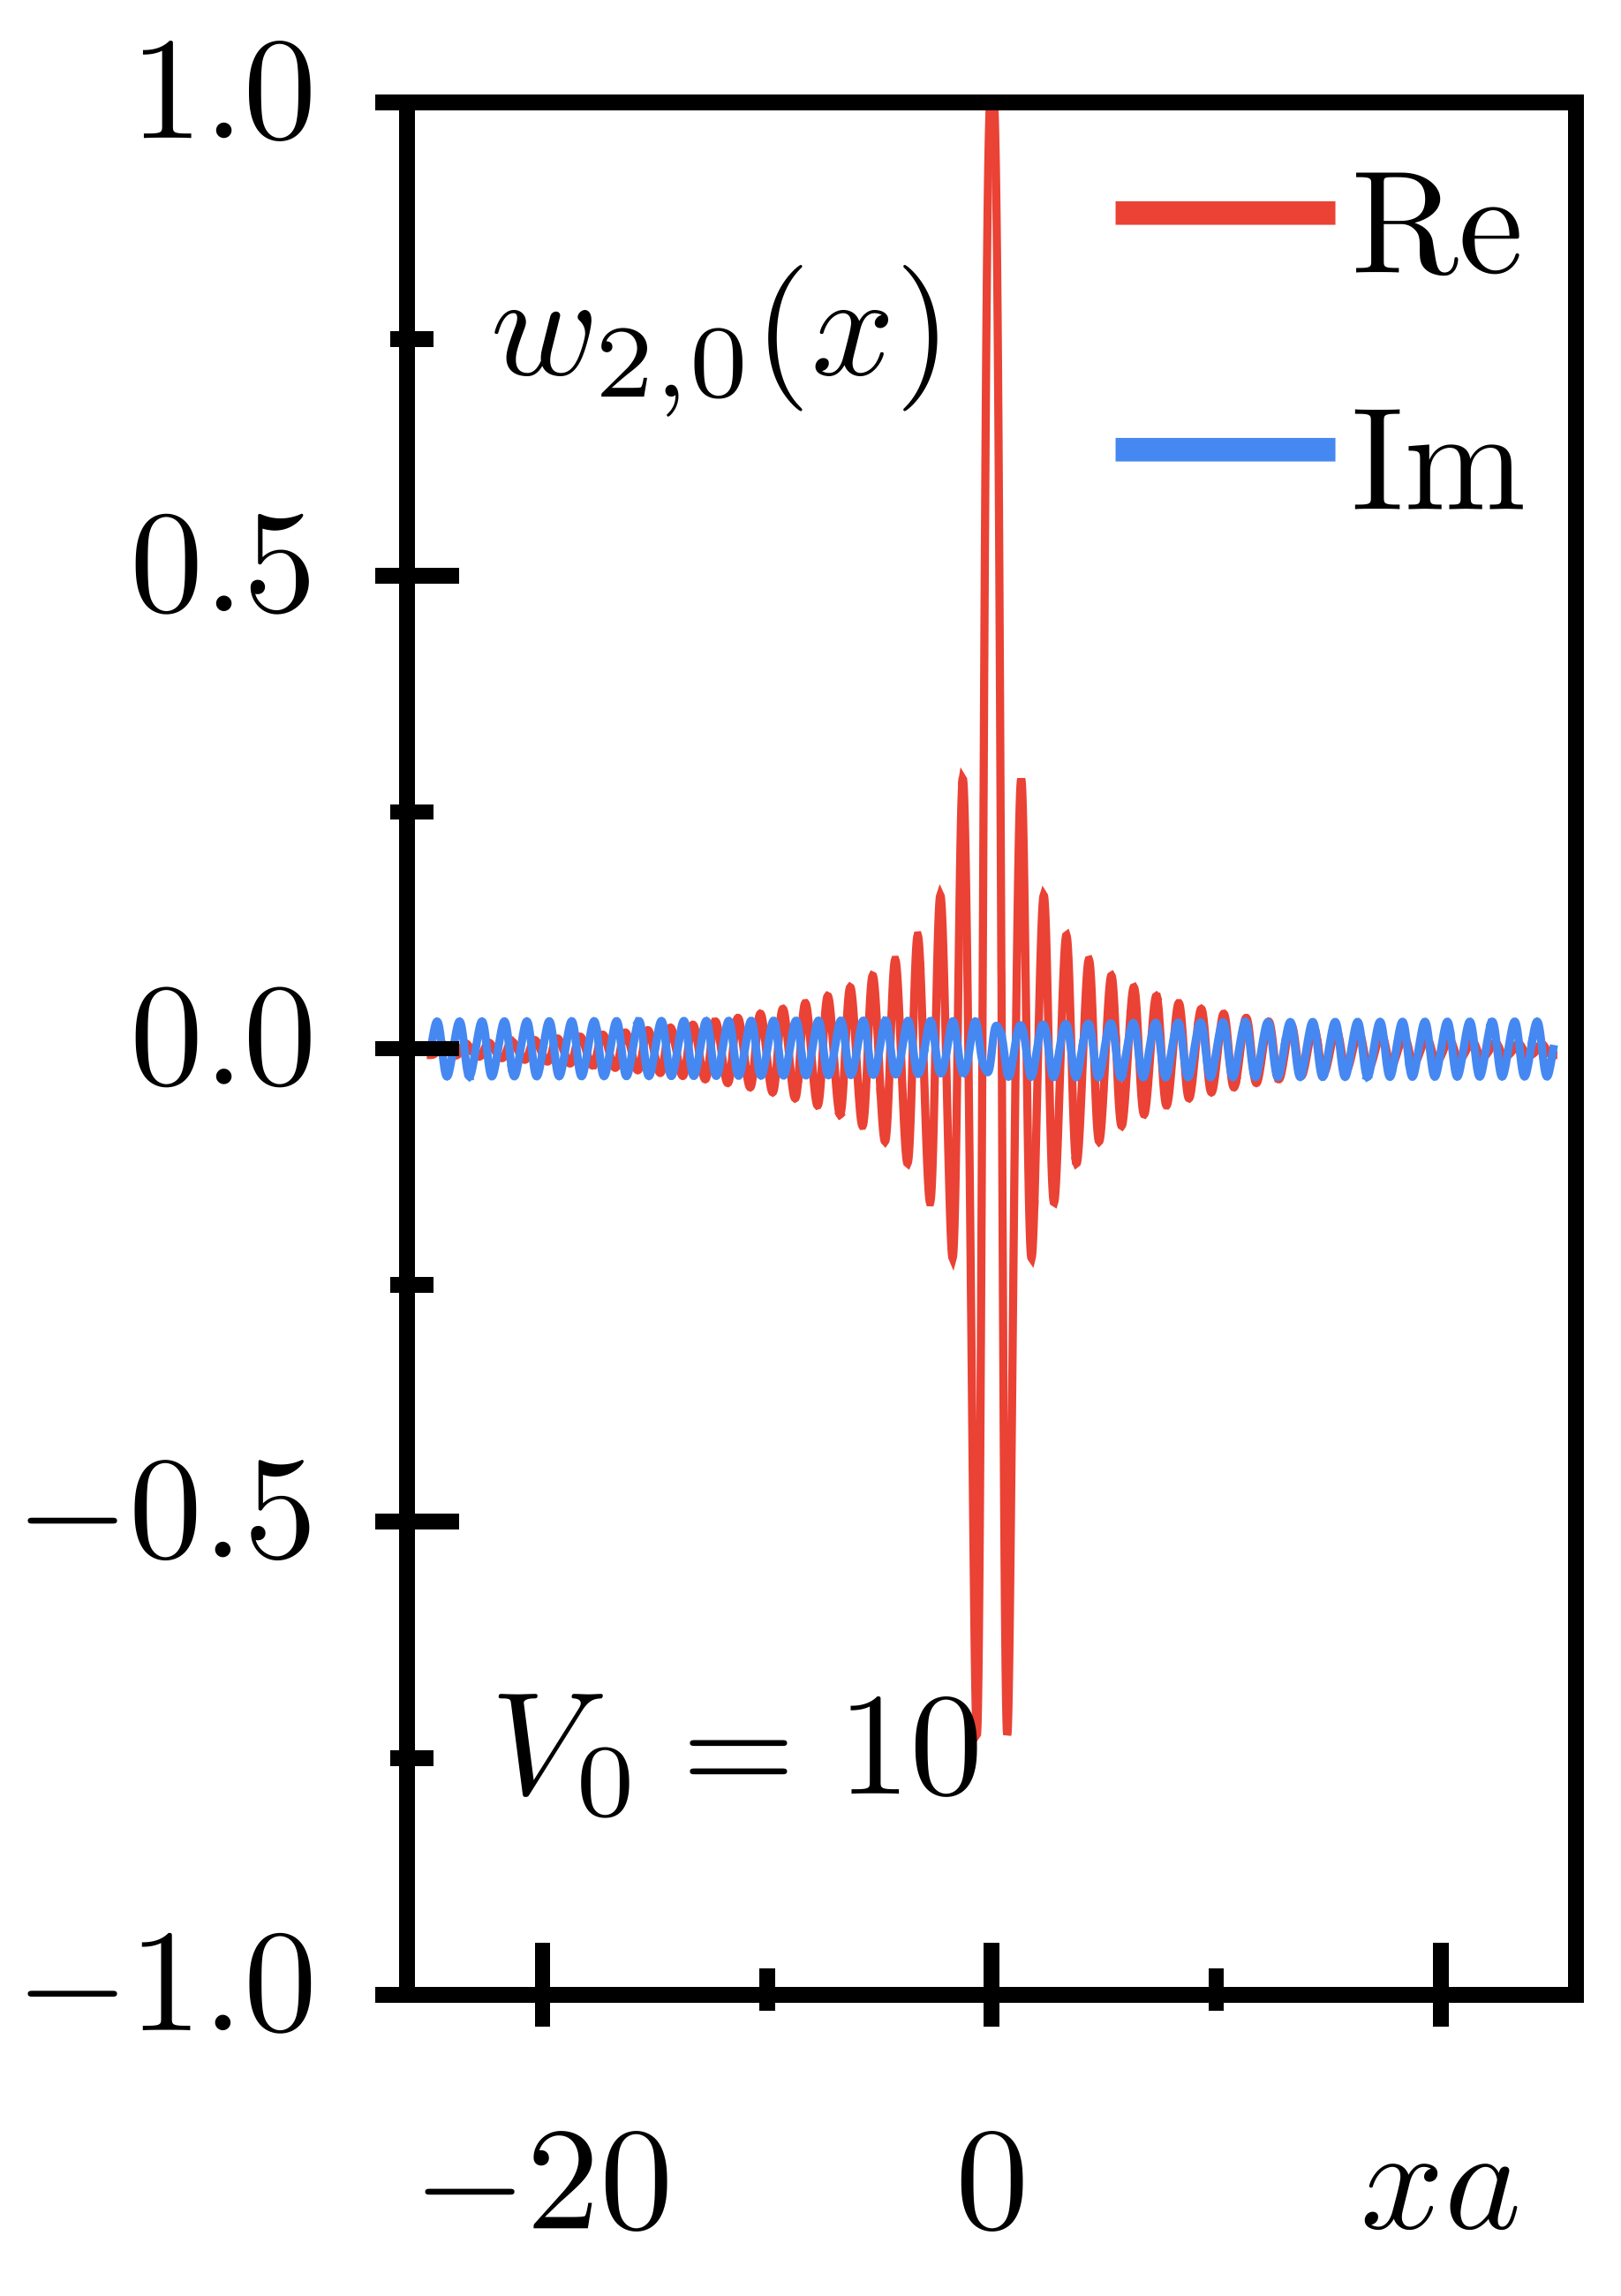
\includegraphics{figures/wannier2_10.png}}
    \subfigure[]{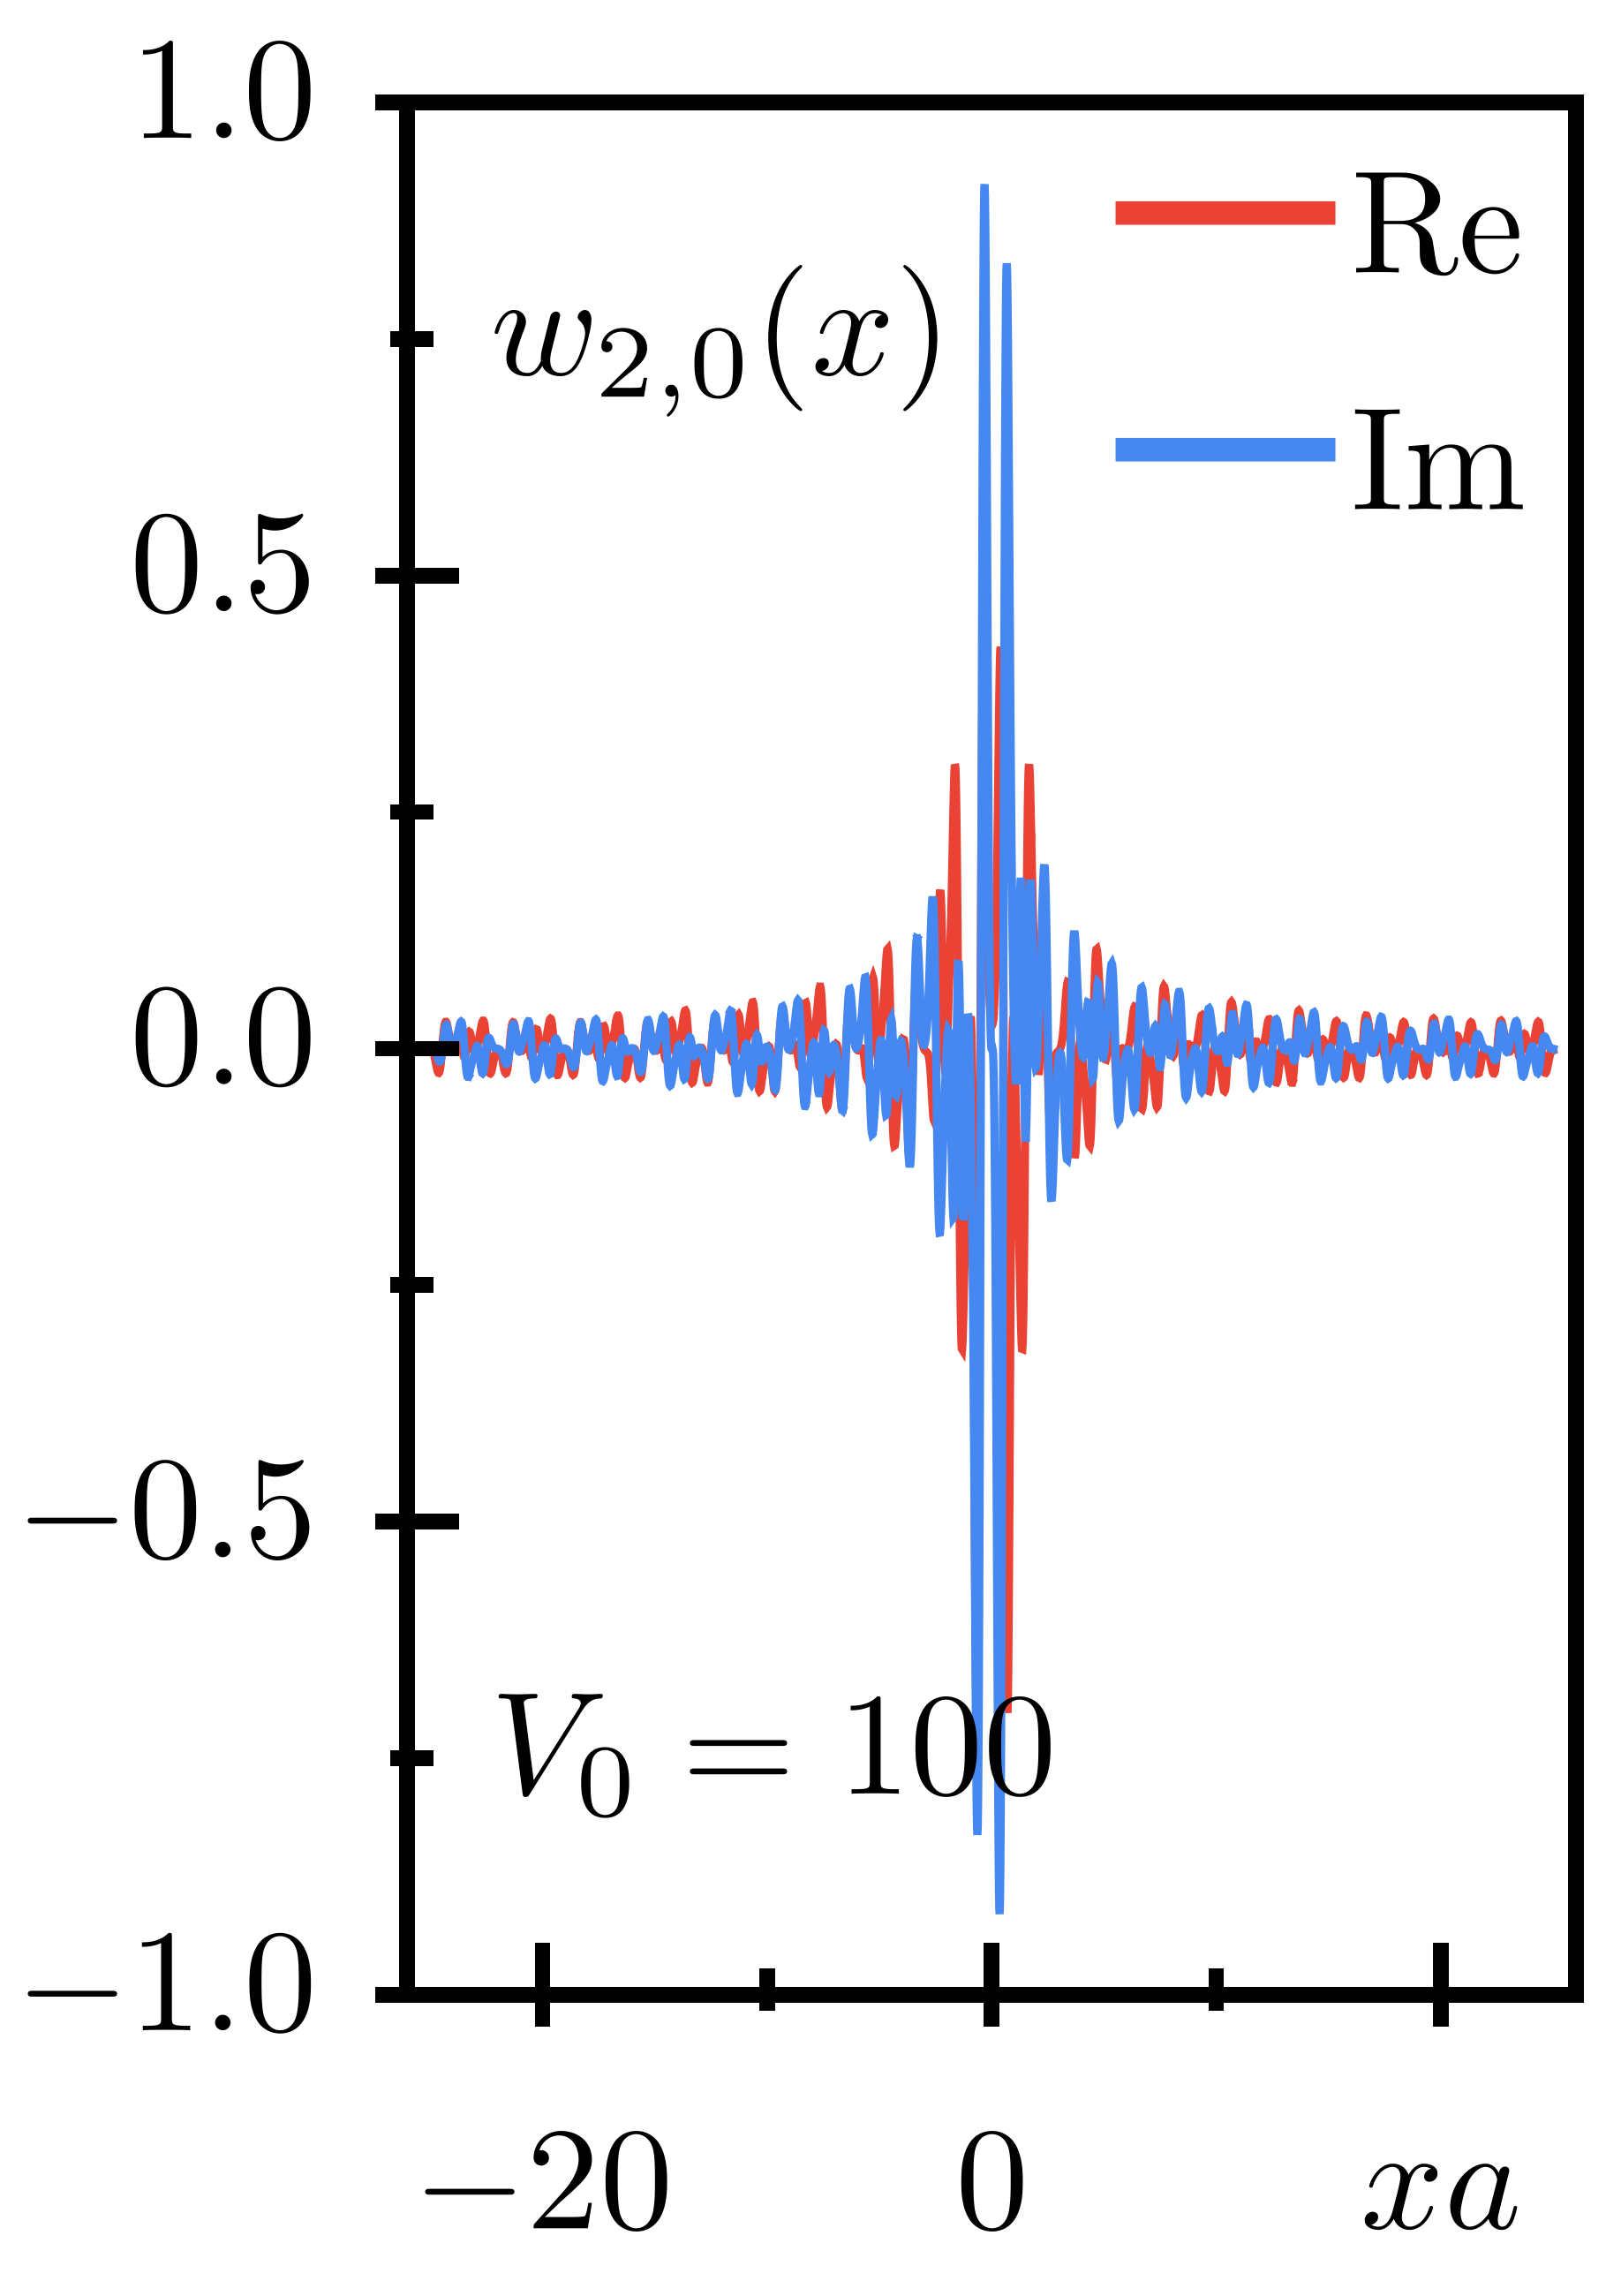
\includegraphics{figures/wannier2_100.png}}\\
    \caption{Example Wannier functions of the first two bands for a periodic potential of the form $V_{ae}(x)=V_0\sin(2\pi/ax)$ for different potential depth. The integration of the Bloch states was performed by assuming a periodicity over $L=50$ lattice translations.}
    \label{fig:tight_binding_wanniers}
\end{figure}

For this purpose, we assume the problem of the single-particle Hamiltonian $\hat H_0$ to be fully solved, such that the Bloch states $\psi_{\alpha{\bf k}}$ are determined, diagonalize $\hat H_0$ and have energy eigenvalues $\varepsilon_{\alpha{\bf k}}$.
This allows to introduce the Wannier basis -- a localized basis composed of the Bloch states and defined as
\begin{align}
    \ket{w_{\alpha{\bf R}}} = \frac1{\sqrt N}\sum_{\bf k}\re^{-\ri{\bf k}{\bf R}}\ket{\psi_{\alpha{\bf k}}}.
    \label{eq:wannier_states}
\end{align}
Note that every momentum-resolved Bloch function can be multiplied with a complex phase without changing its properties.
This naturally provides a gauge freedom to optimize the Wannier function's properties -- for instance, the construction of a maximally localized basis~\cite{Marzari2012}.
Without going into detail about optimizing Wannier functions, I want to present a basic visualization of these localized states.
For this purpose, let us consider a cosine periodic potential
\begin{align}
    V_{ae}(x) = V_0\cos\brlr{\frac{2\pi}a x}
\end{align}
which yields a particular easy (a tridiagonal Toeplitz) matrix equation for the Bloch vectors presented in \cref{eq:periodic_lattices_numerics}.
To obtain the Wannier functions, we gauge every Bloch function to be purely real at $x=0$, resulting in the examples displayed in \cref{fig:tight_binding_wanniers}.

The existence of localized Wannier states is translated to the language of second quantization by the notion that transformations between a Bloch and Wannier basis are always unitary.
Hence, annihilation and creation operators of Wannier and Bloch states are set in relation by
\begin{align}
    \hat a^\dag_{\alpha{\bf R}s} = \frac1{\sqrt N}\sum_{\bf k}\re^{-\ri{\bf k}{\bf R}}\hat a^\dag_{\alpha{\bf k}s},
    \quad
    \hat a^\dag_{\alpha{\bf k}s} = \frac1{\sqrt N}\sum_{\bf R}\re^{+\ri{\bf k}{\bf R}}\hat a^\dag_{\alpha{\bf R}s}.
    \label{eq:wannier_states_2}
\end{align}
Since the non-interacting Hamiltonian is diagonal in the Bloch basis, the Bloch basis are eigenfunctions with energies $\varepsilon_{\alpha{\bf k}} = \int\rd^dr\, \psi_{\alpha{\bf k}}^* \hat H_0 \psi_{\alpha{\bf k}}$.
In particular, the Hamiltonian is readily cast into the localized basis according to
\begin{align}
    \hat H_0
    =
    \sum_{{\bf k},s}\varepsilon_{\alpha{\bf k}}\hat a^\dag_{\alpha{\bf k}s}\hat a^\pdag_{\alpha{\bf k}s}
    \overset{\text{\cref{eq:wannier_states_2}}}{=}
    \frac1N\sum_{\bf R, R', k}
    \re^{\ri{\bf k}\brlr{{\bf R}-{\bf R'}}}
    \varepsilon_{\alpha{\bf k}}
    \hat a^\dag_{\alpha{\bf R}s}\hat a^\pdag_{\alpha{\bf R'}s}
    =
    \sum_{i, j}T_{\alpha,i,j}
    \hat a^\dag_{\alpha{\bf R}_is}\hat a^\pdag_{\alpha{\bf R}_js}.
    \label{eq:tight_binding_hamiltonian}
\end{align}
The matrix $T_{\alpha}$ contains all amplitudes of transition processes between two lattice centers, to be determined through the dispersion relation of the $\alpha$-band
\begin{align}
    T_{\alpha,i,j} \coloneqq \frac1N\sum_{\bf k}\re^{\ri{\bf k}\brlr{{\bf R}_i-{\bf R}_j}}\varepsilon_{\alpha{\bf k}}.
\end{align}
On an abstract level, the tight binding Hamiltonian denotes quantum particles hopping between lattice sites, connected through the matrix elements $T_{\alpha,i,j}$.
Without quantitative computations of the transition probabilities, we can fix the matrix to $T_{\alpha,i,j}=\sum_rt_{\alpha,r}\delta_{i-r,j} + \hc$ with some constants $t_{\alpha,r}$.
The relation \cref{eq:tight_binding_hamiltonian} has strong implications on the analytic form of the dispersion relation $\varepsilon_{\alpha{\bf k}}$ -- it is fully determined through the geometry of the crystal lattice.
For instance, one-dimensional lattices with single atom unit cells and lattice spacing $a$ have the particularly easy solution
\begin{align}
    \varepsilon_{\alpha k} = \sum_r 2t_r\cos(r ka).
    \label{eq:1D_tight_binding_dispersion}
\end{align}
Note that this equation is consistent with the Kronig-Penney dispersion relation in the tight-binding limit, presented in \cref{eq:kronig_penney_tight_binding_dispersion}.
In higher dimensions, the evaluation of the dispersion relation may become lengthy, but remains always analytic.

Oftentimes, a single-band approximation is established to fix (and drop) the band index $\alpha$.
This situation is achieved in case the bottom band is sufficiently separated from the second (e.g. through a strong on-site lattice potential).
A corresponding two-body interaction $\hat V_{ee}$ in the single-band approximation reads
\begin{align}
    \hat V_{ee} = \frac12\sum_{i,i',j,j'}\sum_{s,s'}V_{i,i',j,j'}\hat a^\dag_{{\bf R}_is}\hat a^\dag_{{\bf R}_{i'}s'}\hat a^\pdag_{{\bf R}_js'}\hat a^\pdag_{{\bf R}_{j'}s}.
\end{align}
The matrix elements of the interaction are given by the integral expressions
\begin{align}
    V_{i,i',j,j'} = \int\rd^dr\int\rd^dr'\,w^*_{{\bf R}_i}({\bf r})w^*_{{\bf R}_{i'}}({\bf r}')w_{{\bf R}_j}({\bf r}')w_{{\bf R}_{j'}}({\bf r})V_{ee}({\bf r-r'}).
    \label{eq:two_body_interaction_transition_rates}
\end{align}
The explicit determination of the matrix elements requires knowledge of the form of the Wannier states which, for real materials, is an active field of research on its own.
However, these states are localized and as such the transition rate integrals are short-ranged in most cases.
For this reason, it is sufficient to account for transitions and interactions up to nearest neighbors
\begin{align}
    T_{i,j} \approx \mu\delta_{i,j} + t\delta_{i-1,j}+t^*\delta_{i+1,j},
    \quad
    V_{i,i',j,j'} \approx U\delta_{i,j'}\delta_{i',j}\delta_{i,i'} + V\delta_{i,j'}\delta_{i',j}(\delta_{i-1,i'}+\delta_{i+1,i'}).
\end{align}
In summary, we are at liberty to slightly simplify the notation and arrive at the family of Hubbard-type models, written in second quantization
\begin{align}
    \hat H_{\rm Hubbard} = \sum_{i,s}\brlr{t \hat a^\dag_{i,s}\hat a^\pdag_{j+1,s} + \hc} + \frac U2\sum_{i,s,s'}\hat n_{i,s}\hat n_{i,s'} + V\sum_{i,s,s'}\hat n_{i,s}\hat n_{i+1,s'}.
    \label{eq:hubbard_hamiltonian}
\end{align}
The operator $\hat a_{i,s}$ annihilates a Wannier state of flavor $s$, localized around the $i$'th lattice position.

In the above derivation, I do not comment on the nature of $t$ which can be assumed to be real for traditional Hubbard models.
If, however, the geometry of the tight binding approximation is sufficiently complex, i.e. if the matrix $T$ spans a higher dimensional lattice, complex transition amplitudes give rise to nontrivial fluxes penetrating the lattice which may alter the underlying physics.
One example for a $2$D system with complex tunneling elements is the Harper-Hofstadter model~\cite{Hofstadter1976}, realized by artificial gauge fields induced by laser-assisted tunnelings in ultracold atomic lattice systems~\cite{Aidelsburger2016}.
The nonzero fluxes in this model mimic the effect of charged particles moving in a magnetic field, based on Peierl's substitution~\cite{Peierls1933}.
A more simplified explanation compared to the original work by Rudolf Peierls is based on the infamous Feynman lecture series, book III chapter 21~\cite{feynmanlecturesonline} and adopted from~\cite{WikiPeierls}.
\todo{Wrap up Peierl's substitution here.}

Perhaps the most successful description of electrons in solids is band theory -- based on screened many-body interactions described by effective one-body potentials.
This results in a form of \cref{eq:hubbard_hamiltonian} without density-density interactions such that a diagonalization of the hopping matrix $T$ solves the problem.
However, due to its intrinsic single-particle character, band theory cannot reliably capture truly many-body features such as band magnetism or Mott-to-metal-insulator transitions.
This motivates the study of Hubbard-type models: despite being a brutal simplification of the true two-body interaction, they are the easiest systems that provide an explanation of such interaction-driven features.
Although its apparent innocence, there is no universal treatment of Hubbard models in general.
In one spacial dimension, the Hamiltonian can be solved analytically and thus falls in the category of being ``integrable''~\cite{Essler2005}.
In general, integrability is a quite fragile property and even slight perturbations will break it.
The models we study in the next chapters, albeit closely related to the one-dimensional Hubbard model, do not categorize as integrable due to the presence of additional terms that break some of its fundamental symmetries (e.g. the conservation of the particle flavor).
This motivates the use of alternative methods to study the properties of interacting tight binding models.
One of the most prominent and useful analytic concepts in one dimension is the theory of Luttinger liquids (paired with renormalization group theory) which approximates the microscopic model in the low temperature limit.
%
%
%%%%%%%%%%%%%%%%%%%%%%%%%%%%%%%%%%%%
\section{Tomonaga Luttinger liquids}
\label{sec:tomonaga_LL}
%%%%%%%%%%%%%%%%%%%%%%%%%%%%%%%%%%%%
Luttinger liquids provide a viable tool to study the low-temperature properties of many systems in one and two dimensions.
I start by giving a basic overview on the mapping from spinless fermions to particle-hole excitations in the vicinity of the Fermi points before I introduce the more general formulas for spinful models.
We are interested in building an effective model in one dimension capturing the relevant degrees of freedom at low temperatures.
With that purpose, let us start with the free fermionic 1D Hamiltonian $\hat H_0$ denoted by the following (diagonal) representation in momentum space
\begin{align}
    \hat H_0 = \sum_k \frac{(\hbar k)^2}{2m}\hat n_k
    \label{eq:hamiltonian_free_particles}
\end{align}
with dispersion relation $\varepsilon_k =\frac{k^2}{2m}$ depicted in \cref{fig:1D_quadratic_dispersion}.
\begin{figure}
    \centering
    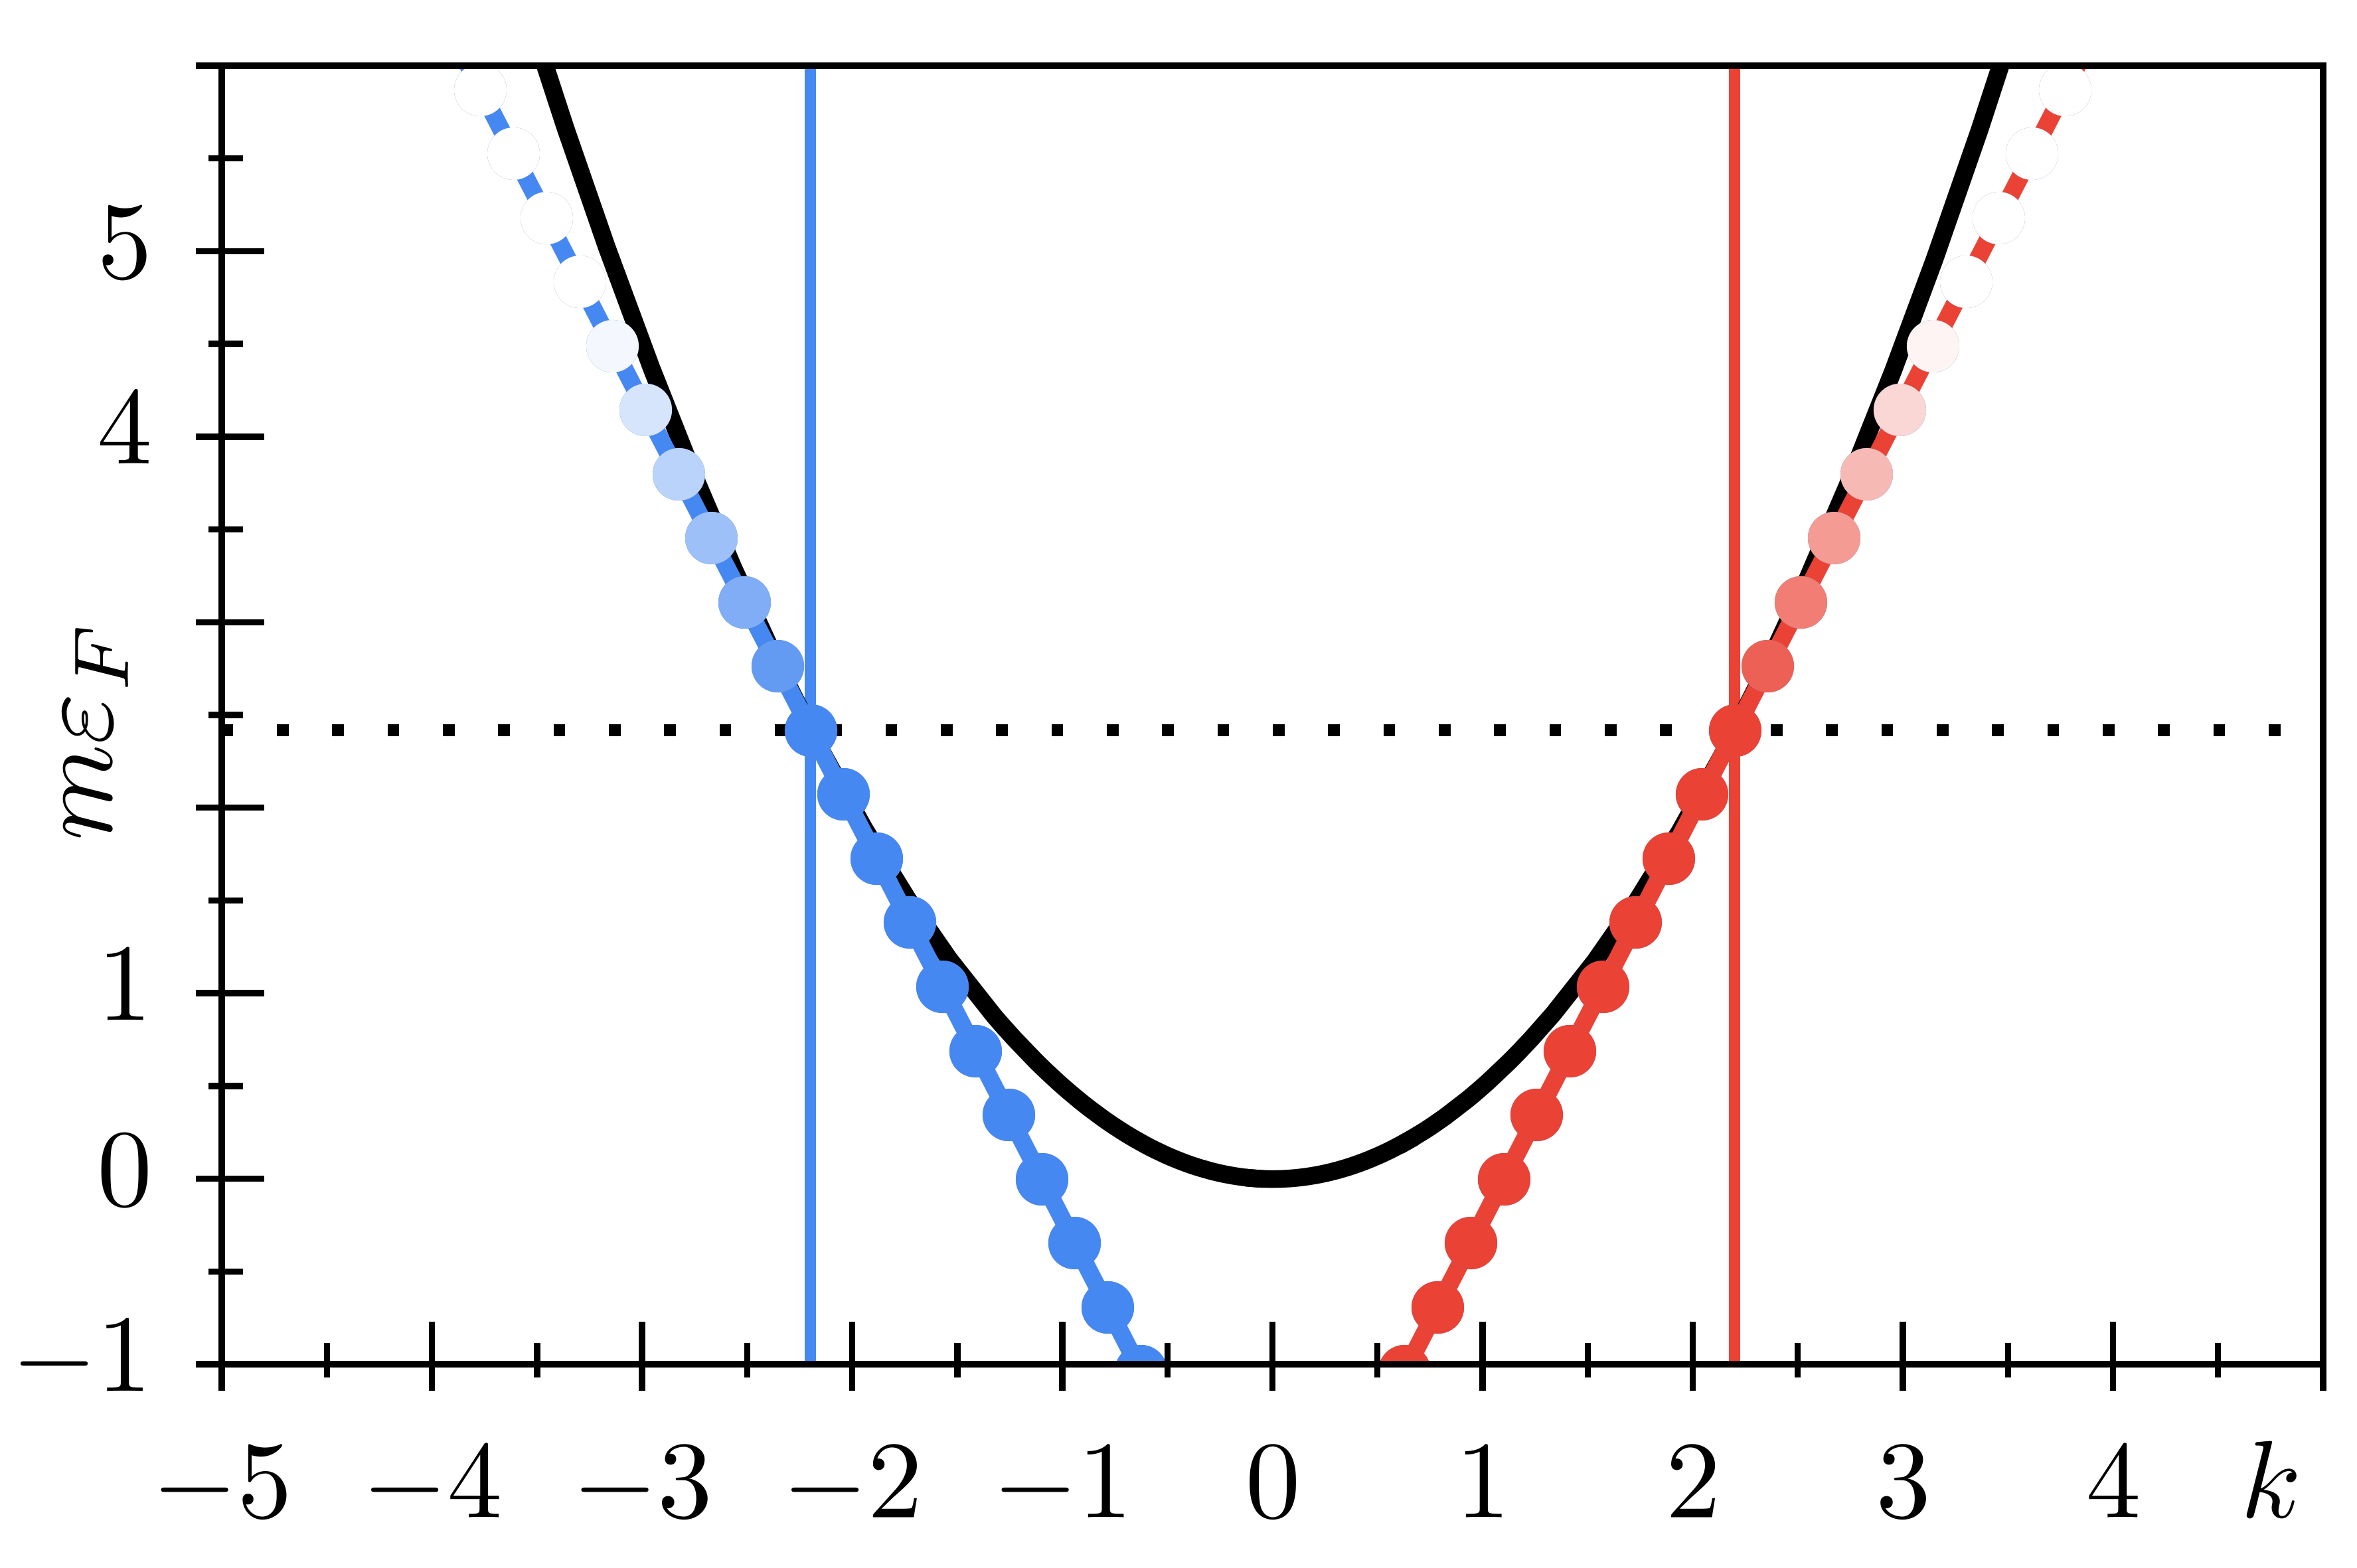
\includegraphics{figures/1D_quadratic_dispersion.png}
    \caption{Quadratic dispersion relation with approximations close to the Fermi energy $\varepsilon_F$.}
    \label{fig:1D_quadratic_dispersion}
\end{figure}
Close to the Fermi energy $\varepsilon_F\coloneqq\varepsilon_{\pm k_F}$, we can approximate the free dispersion and obtain a system of two different species
\begin{align}
    \hat H_0
    &= \sum_k \hbar^2\brlr{\varepsilon_F \pm \frac{k_F}{m}(k\mp k_F) + \mathcal{O}(k^2)}\hat n_k
    \\
    &= \sum_q \hbar^2\brlr{\varepsilon_F + \frac{k_F}{m}q\brlr{\hat n_{q+k_F}-\hat n_{q-k_F}} + \mathcal{O}(k^2)}
    \approx \sum_{q} v_F \hbar q \brlr{\hat c^\dag_{q,R}\hat c^\pdag_{q,R} - \hat c^\dag_{q,L}\hat c^\pdag_{q,L}}
    \label{eq:dispersion_linearization}
\end{align}
which implies a restriction of $q$ to a small window $|q|<\Gamma\ll m\varepsilon_F$ beyond which \cref{eq:dispersion_linearization} is considered invalid.
Note the introduction of the so-called right and left operators $\hat c_{R/L,q}$ which annihilate particles propagating to the left/right with Fermi velocity $\pm v_F=\hbar k_F/m$.

For the next part, it will be convenient to understand the meaning of the local density in momentum space, i.e.
\begin{align}
    \hat n(x) = \hat c^\dag_x \hat c^\pdag_x = \frac1L\sum_{k,q}\re^{-\ri x q}\hat c^\dag_{k+q}\hat c^\pdag_{k}.
    \label{eq:local_density}
\end{align}
$\hat n(x)$ thus creates a superposition of particle-hole pairs with characteristic wavelength $q^{-1}$.
The number of particle-hole pairs can be counted through the operator
\begin{align}
    \hat \rho_{-q}\coloneqq \sum_k \hat c^\dag_{k-q}\hat c^\pdag_{k}.
\end{align}
Note further that $\hat\rho_q^\dag = \hat\rho_{-q}$.
By confining the theory close to the Fermi points, there are only two different classes of particle-hole excitations with $q\approx 0$ and $q\approx2k_F$.
The long-wavelength excitations $q\approx0$ are particle-hole pairs of the same species (left or right movers), and excitations of $q\approx2k_F$ are particle-hole pairs of a mixture of the two.
This implies drastic consequences on the relevant action of operators, which we will see in the following.
Let us note here that the density operator of the left/right species $\hat\rho_{\tau,q}$, $\tau\in\{L,R\}$ applied to a Fermi sea creates stable particle-hole excitations (i.e. particles and holes propagate with the same velocity $\pm v_F$) and can thus be used to construct a complete basis of the subspace $\FS^N$ -- for this rather dry discussion, I refer to~\cite{vonDelft1998}.
The consequences of the approximation in \cref{eq:dispersion_linearization} is easily understood for the single-particle operators
\begin{align}
    \hat c^\dag_x = \frac1{\sqrt L}\sum_k \re^{-\ri k x}\hat c^\dag_k \approx \frac1{\sqrt L}\sum_{|q|<\Gamma}\re^{-\ri (q+k_F) x}\hat c^\dag_{R, q} + \re^{-\ri (q-k_F) x}\hat c^\dag_{L, q}
    \label{eq:confinement_creation_annihilation}
\end{align}
which is then used to find the local density
\begin{align}
    \hat n(x)
    &\approx \frac1L\sum_{q,q'}\brlr{\re^{-\ri (q+k_F) x}\hat c^\dag_{R, q} + \re^{\ri (k_F-q) x}\hat c^\dag_{L, q}}\brlr{\re^{\ri (k_F+q') x}\hat c^\pdag_{R, q'} + \re^{-\ri (k_F-q') x}\hat c^\pdag_{L, q'}},
    \\
    &= \hat \rho_R(x) + \hat \rho_L(x) + \re^{-2\ri k_F}\hat c^\dag_{R}(x)\hat c^\pdag_{L}(x) + \re^{2\ri k_F}\hat c^\dag_{L}(x)\hat c^\pdag_{R}(x).
    \label{eq:local_density_approximation}
\end{align}
The first two terms correspond to the $q\approx0$ part of the density, and scattering occurs on the same side of the dispersion relation.
The last two terms scatter right with left movers and transfer particles from one side to the other, which appear at $q\approx2k_F$.

We now turn to an arbitrary two-body interaction of the form~\cref{eq:two_point_interaction} which reads
\begin{align}
    \hat V
    % &= \frac12\int\rd x'\int\rd x V(x'-x)c^\dag(x')c^\dag(x)c^\pdag(x)c^\pdag(x')
    % \\
    &= \frac12\int\rd r\int\rd x V(r)\hat c^\dag(r+x)\hat c^\dag(x)\hat c^\pdag(x)\hat c^\pdag(r+x),
    \\
    &= \frac1{2L^2}\sum_{kk'll'}\int\rd r\int\rd x V(r)\re^{-\ri r(k-l')}\re^{-\ri x(k-l'+k'-l)}\hat c^\dag_k\hat c^\dag_{k'}\hat c^\pdag_l\hat c^\pdag_{l'},
    % \\
    % &= \frac1{2L}\sum_{kk'lq}\int\rd r V(r)\re^{-\ri rq}\delta_{l,k'+q}c^\dag_kc^\dag_{k'}c^\pdag_lc^\pdag_{k-q}
    \\
    &= \frac1{2L}\sum_{kk'q}V(q)\hat c^\dag_k\hat c^\dag_{k'}\hat c^\pdag_{k'+q}\hat c^\pdag_{k-q}
    = \frac1{2L}\sum_{q}V(q)\hat\rho_q\hat\rho^\dag_{q} - \mu.
    \label{eq:two_body_interaction_momentum_space}
\end{align}
The last term is just a constant $\mu = \frac N{2L}\sum_qV(q)$ and can thus be neglected.
By imposing that relevant contributions act close to the Fermi energy involving only momenta in the interval $|k|\in\{k_F\pm\Gamma\}$, we can split the sum in two contributions, one involving scattering processes at small and the other scattering at large momenta
\begin{align}
    \hat V \approx \frac1{2L}\sum_{q\approx0}V(q)\hat\rho_{q}\hat\rho^\dag_{q} + \sum_{q\approx2k_F}V(q)\hat\rho_{q}\hat\rho^\dag_{q}.
\end{align}
For a later study, it is important to note that the amplitude of the two different $q\approx0$ processes, denoted by $V(q\approx0)$, is equal and independent of the form of the interaction.
A full classification of hypothetical scattering processes is given in~\cref{fig:scattering_processes}.
\begin{figure}
    \centering
    \subfigure[]{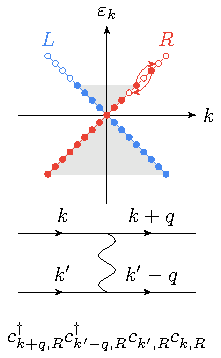
\includegraphics[width=0.328\textwidth]{figures/g4_right.pdf}}
    \subfigure[]{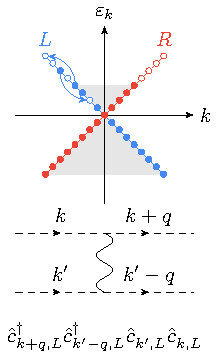
\includegraphics[width=0.328\textwidth]{figures/g4_left.pdf}}
    \subfigure[]{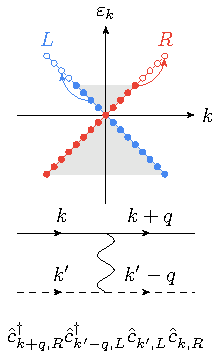
\includegraphics[width=0.328\textwidth]{figures/g2.pdf}}
    \subfigure[]{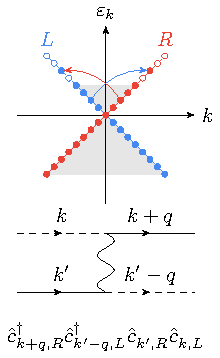
\includegraphics[width=0.328\textwidth]{figures/g1.pdf}}
    \subfigure[]{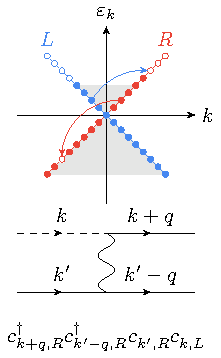
\includegraphics[width=0.328\textwidth]{figures/g13.pdf}}
    \subfigure[]{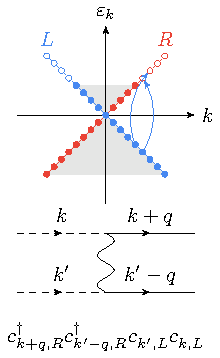
\includegraphics[width=0.328\textwidth]{figures/g22.pdf}}
    \caption{Relevant scattering processes of a generic density-density interaction in one-dimensional quantum systems. (a)/(b) The depicted scattering is commonly referred to as ``forward scattering'' $g_4$ process ($4$ right/left operators, $q\approx0$), (c) as ``backscattering'' $g_2$ process (containing $2$ pairs of right and left operators, $q\approx0$) and (d) as ``Umklapp'' process $g_1$ with momentum transfer $q\approx 2k_F$. Other possible scatterings like the ones depicted in (e) and (f) require the existence of high-energy excitations and are thus exponentially suppressed at low temperatures.}
    \label{fig:scattering_processes}
\end{figure}
This simple argumentation allows to consider only the most relevant processes at low temperatures, i.e. those presented in panels (a) - (d).
We will call those processes forward scattering (note that we are discarding chemical potentials on the right hand side of the following equations)
\begin{align}
    g_4\sum_{k,k',q}\hat c^\dag_{k+q,\tau}\hat c^\dag_{k'-q,\tau}\hat c^\pdag_{k',\tau}\hat c^\pdag_{k,\tau} = g_4 \sum_q\hat\rho^\pdag_{q,\tau}\hat\rho^\dag_{q,\tau},
\end{align}
backscattering
\begin{align}
    g_2\sum_{k,k',q}\hat c^\dag_{k+q,\tau}\hat c^\dag_{k'-q,\overline\tau}\hat c^\pdag_{k',\overline\tau}\hat c^\pdag_{k,\tau} = g_2\sum_q \hat\rho^\pdag_{q,\tau}\hat\rho^\dag_{q,\overline\tau}
\end{align}
and Umklapp scattering
\begin{align}
    g_1\sum_{k,k',q} \hat c^\dag_{k+q,\tau}\hat c^\dag_{k'-q,\overline\tau}\hat c^\pdag_{k',\tau}\hat c^\pdag_{k,\overline\tau}.
\end{align}
I make one important remark on the Umklapp scattering of spinless fermions, that is
\begin{align}
    \sum_{k,k',q}V(q)
    \hat c^\dag_{k+q,\tau}\hat c^\dag_{k'-q,\overline\tau}\hat c^\pdag_{k',\tau}\hat c^\pdag_{k,\overline\tau}
    =
    \sum_{k,k',q,q'}V(q) \delta_{q,q'-k+k'}
    \hat c^\dag_{k'+q',\tau}\hat c^\dag_{k-q',\overline\tau}\hat c^\pdag_{k',\tau}\hat c^\pdag_{k,\overline\tau}
    \\
    =
    -\sum_{k,k',q}V(k'-k+q)\hat c^\dag_{k+q,\tau}\hat c^\dag_{k'-q,\overline\tau}\hat c^\pdag_{k',\overline\tau}\hat c^\pdag_{k,\tau}
    \approx -V(2k_F)\sum_q\hat\rho^\pdag_{q,\tau}\hat\rho^\dag_{q,\overline\tau}.
\end{align}
This proofs that Umklapp terms are up to a sign equivalent to backscattering terms in case of indiscernible particles.
Interestingly, the $2k_F$ components of forward scatterings can be reordered in the same manner\footnote{This is interesting because one is inclined to neglect the $2k_F$ forward scattering processes at first sight. The reordering demonstrates that $q\approx0$ are equivalent to $2k_F$ scatterings such that both have to be accounted for on equal grounds.}, such that we find the identity $g_4 = g_2 \approx V(0)-V(2k_F)$.
% Umklapp terms cannot be expressed in the density operators of the moving modes $\hat\rho_{q,\tau}$ and, for this reason, are discarded here\footnote{Later, we will see that the Umklapp term in the spinless case are ``marginal'' and can be disregarded under certain conditions.}.
Other processes like those depicted in \cref{fig:scattering_processes} (e) and (f) require the existence of high-energy excitations and can thus be neglected for the effective low temperature theory developed here.
In summary, we can express the interaction in terms of the density-density operators as
\begin{align}
    \hat V \approx \frac{\hbar}{2L}\sum_{q,\tau}\brlr{g_4\hat\rho^\pdag_{q,\tau}\hat\rho^\dag_{q,\tau} + g_2\hat\rho^\pdag_{q,\tau}\hat\rho^\dag_{q,\overline\tau}}
    =
    \frac{\hbar}{L}\sum_{q>0}
    \begin{pmatrix}
        \hat\rho^\pdag_{q,R} & \hat\rho^\pdag_{q,L}
    \end{pmatrix}
    \begin{pmatrix}
        g_4 & g_2 \\
        g_2 & g_4
    \end{pmatrix}
    \begin{pmatrix}
        \hat\rho_{-q,R} \\ \hat\rho_{-q,L}
    \end{pmatrix}
    .
    \label{eq:interaction_densities}
\end{align}
To proceed further, it will be useful to compute the commutation of the density operators
\begin{align}
    \commutator{\hat\rho_{q,\tau},\hat\rho_{q',\tau'}}
    =
    \delta_{\tau,\tau'}\sum_k\brlr{\hat c^\dag_{k+q,\tau}\hat c^\pdag_{k-q',\tau}-\hat c^\dag_{k+q+q',\tau}\hat c^\pdag_{k,\tau}}
    \approx
    -\sigma_\tau\delta_{\tau,\tau'}\delta_{q,-q'}\frac{qL}{2\pi}
    \label{eq:chiral_density_commutation}
\end{align}
in which $\sigma_\tau=\pm1$ for $\tau=R/L$, respectively, and the right hand side is obtained through a projection on the ground state\footnote{This is a reasonable approximation for small interactions only (as a result from a first order perturbative expansion).
For a more thorough discussion of \cref{eq:chiral_density_commutation}, see~\cite{Giamarchi2003}.}.
We are now in shape to define canonical bosonic operators representing the interaction degrees of freedom for $q>0$
\begin{align}
    \hat b^\dag_{+q} \coloneqq \sqrt\frac{2\pi}{qL}\hat\rho_{-q,L},
    \quad
    \hat b^\pdag_{+q} \coloneqq \sqrt\frac{2\pi}{qL}\hat\rho_{+q,L},
    \\
    \hat b^\dag_{-q} \coloneqq \sqrt\frac{2\pi}{qL}\hat\rho_{+q,R},
    \quad
    \hat b^\pdag_{-q} \coloneqq \sqrt\frac{2\pi}{qL}\hat\rho_{-q,R},
    \label{eq:canonical_bosonic_operators}
\end{align}
that satisfy the commutation relation $\commutator{\hat b_q^\pdag,\hat b_{q'}^\dag} = \delta_{q,q'}$.
Using \cref{eq:canonical_bosonic_operators} results in a familiar expression for the interaction written in \cref{eq:interaction_densities}, i.e.
\begin{align}
    \hat V \approx\sum_{q>0}\frac{\hbar q}{2\pi}
    \begin{pmatrix}
        \hat b_q & \hat b^\dag_{-q}
    \end{pmatrix}
    \begin{pmatrix}
        g_4 & g_2 \\
        g_2 & g_4
    \end{pmatrix}
    \begin{pmatrix}
        \hat b^\dag_q \\ \hat b_{-q}
    \end{pmatrix}
    .
    \label{eq:quadratic_interactions}
\end{align}
The interaction, originally quartic in the fermionic degrees of freedom, can be cast into a (quadratic) sum of bosonic operators which are the low-energy excitations of the original model.
All that is left to do is to cast the kinetic term into this new basis, which is actually a quite lengthy calculation if we were to approach it by brute-force.
There is an indirect reasoning through Schur's lemma: if two operators $\hat H$ and $\hat H'$ have identical commutation relations with all $\{c^\pdag_\alpha,c^\dag_\alpha\}$, then the two operators are equal up to a chemical potential.
One can easily verify the commutator of the mover-density with the kinetic Hamiltonian
\begin{align}
    \commutator{\hat H_0, \hat\rho_{q,\tau}}
    =
    \sum_{p,\tau'}v_F\sigma_{\tau'}\hbar \commutator{\hat n_{p,\tau'},\hat\rho_{q,\tau}}
    =
    \sigma_\tau v_F \hbar q \hat\rho_{q,\tau}
\end{align}
and find its equivalent expression in bosonic degrees of freedom to be
\begin{align}
    \hat H_0' = \frac{\hbar \pi v_F}L\sum_{q,\tau}\hat\rho_{q,\tau}\hat\rho_{-q,\tau} = \frac{2\hbar\pi v_F}L\sum_{q>0,\tau}\hat\rho_{q,\tau}\hat\rho_{-q,\tau},
\end{align}
which can be verified through evaluation of
\begin{align}
    \commutator{\hat H_0',\hat\rho_{q,\tau}}
    \overset{\text{\cref{eq:recursive_commutation}}}{=}
    -\frac{\hbar \pi v_F}L
    \sum_{p,\tau'}
    \brlr{
    \commutator{\hat\rho_{q,\tau},\hat\rho_{p,\tau'}}\hat\rho_{-p,\tau'}
    -
    \hat\rho_{p,\tau'}\commutator{\hat\rho_{q,\tau},\hat\rho_{-p,\tau'}}
    }
    =
    \sigma_\tau v_F \hbar q\hat\rho_{q,\tau}
\end{align}
and thus we conclude our previous statement $\hat H_0' = \hat H_0 + \mu$ with an irrelevant constant $\mu$.
The effective low energy Hamiltonian containing kinetic and interaction energy satisfies the following matrix equation
\begin{align}
    \hat H = \hat H_0 + \hat V \approx
    \sum_{q>0}\frac{\hbar q}{2\pi}
    \begin{pmatrix}
        \hat b_q & \hat b^\dag_{-q}
    \end{pmatrix}
    \begin{pmatrix}
        2\pi v_F + g_4 & g_2 \\
        g_2 & 2\pi v_F + g_4
    \end{pmatrix}
    \begin{pmatrix}
        \hat b^\dag_q \\ \hat b_{-q}
    \end{pmatrix}
    .
    \label{eq:luttinger_hamiltonian_nondiagonal}
\end{align}
As a final step, we want to find the spectrum of the previous Hamiltonian through a basis transformation $\hat B_q = T \hat B'_q$\footnote{The matrix coupling the dot product of the operator spinors $\hat B_q$ is independent on the momentum $q$ and as such the basis transformation $T$ will not depend on $q$ as well.} with $\hat B_q = (\hat b_q^\dag, \hat b_{-q})^T$ such that
\begin{align}
    \hat H = \sum_{q>0}\hbar q\hat B^\dag_q H \hat B^\pdag_q = \sum_{q>0}\hbar q\hat B'^\dag_q T^\dag H T \hat B'^\pdag_q
\end{align}
is in its diagonal form.
Naive (unitary) rotations do not preserve the commutators of the spinor $\hat B$, defined through
\begin{align}
    \commutator{\hat B_{q,i}^\pdag,\hat B^\dag_{q,j}} = \commutator{\hat B_{q,i}'^\pdag,\hat B'^\dag_{q,j}} = (-\sigma_z)_{i,j}
\end{align}
which imposes an additional constraint on the transformation $T$ according to
\begin{align}
    T^\dag\sigma_z T = \sigma_z,
    \quad
    T^\dag = \sigma_zT^{-1}\sigma_z.
\end{align}
We thus find the similarity relation between the original and the rotated basis according to
\begin{align}
    H'=T^\dag HT =\sigma_z T^{-1}\sigma_z H T,
\end{align}
which allows us to solve the eigenvalue equation of $\sigma_z H$ without knowing the explicit form of $T$.
Since $\sigma_zH$ has vanishing trace, its spectrum is symmetric $\pm E$ and we arrive at the appealing result $H' = u\mathbb1$ with the $2\times2$ unit matrix $\mathbb1$ and scalar eigenvalue
\begin{align}
    u = \frac1{2\pi}\sqrt{\brlr{2\pi v_F + g_4}^2 - g_2^2}
\end{align}
leading to the identity
\begin{align}
    \hat H = \sum_{q>0} u\hbar q \hat B'^\dag_q \hat B'^\pdag_q = \sum_{q>0} \hbar \omega_q \hat B'^\dag_q \hat B'^\pdag_q = \sum_q \hbar  \omega_q \hat b'^\dag_q\hat b'^\pdag_q.
\end{align}
Note that we succeeded to rewrite the original problem to a sum of decoupled harmonic oscillators with frequencies $\omega_q\coloneqq u|q|$.
In particular, assuming two canonically conjugate fields $\commutator{\hat \phi_{k},\hat \pi_{k'}} = \ri\hbar\delta_{k,k'}$, the following substitution of ladder operators, i.e.
\begin{align}
    \hat b'_q = \sqrt{\frac{mw_q}{2\pi\hbar}}\brlr{\hat\phi_q + \frac{\ri}{mw_q}\hat\pi_{-q}},
    \quad
    \hat b'^\dag_q = \sqrt{\frac{mw_q}{2\pi\hbar}}\brlr{\hat\phi_{-q} - \frac{\ri}{mw_q}\hat\pi_{q}},
\end{align}
brings the diagonalized Hamiltonian to the more traditional form
\begin{align}
    \hat H = \sum_q \frac{\hat\pi_q\hat\pi_{-q}}{2\pi m} + \frac{m\omega_q^2}{2\pi}\hat\phi_q\hat\phi_{-q}
    =
    \int\frac{\rd x}{2\pi}\, \brlr{\hat\pi^2/m + {Da^2}(\partial_x\hat\phi)^2}.
\end{align}
In the above, I introduced an effective spring constant through the velocity and lattice spacing $D=mu^2/a^2$.
In particular, the field $\partial_x\hat\phi$ can be interpreted as the position offset from the quasiparticle's equilibrium position and $\hat\pi$ is its effective momentum.
Moving to dimensionless units (by imposing $\hbar=c=1$ and requiring a unit mass) and rescaling the fields $\hat\phi\rightarrow \frac1{uK}\hat\phi$, $\hat\pi\rightarrow uK\hat\pi$ results in the standard Luttinger liquid Hamiltonian
\begin{align}
    \hat H = \int\frac{\rd x}{2\pi}\, \brlr{uK\hat\pi^2 + \frac uK(\partial_x\hat\phi)^2},
    \label{eq:ll_hamiltonian}
\end{align}
in which the couplings are encoded in the dimensionless Luttinger parameters
\begin{align}
    u = v_F\sqrt{\brlr{1 + y_4}^2 - y_2^2},
    \quad
    K = \sqrt{\frac{1+y_4-y_2}{1+y_4+y_2}},
    \quad
    y_4=g_4/(2\pi v_F),
    \quad
    y_2=g_2/(2\pi v_F).
\end{align}
The expressions of the effective fields (after the particular choice of the rescaling by a factor $uK$) in terms of the local creation and annihilation operators result from a quite involved calculation which is particularly clearly presented in several excellent books on the topic~\cite{Bruus2004,Giamarchi2003,Gogolin2004}.
On an intuitive level (given the demonstrated equivalence to the quantum harmonic oscillator), the relation to the local densities is straightforward:
\begin{align}
    \partial_x\hat\phi(x)=-\pi[\hat\rho_R(x)+\hat\rho_L(x)],
    \quad
    \hat\pi(x)=\partial_x\hat\theta=\pi[\hat\rho_R(x)-\hat\rho_L(x)].
\end{align}
These identities, combined with \cref{eq:local_density_approximation} are most practical to implement the concept of Luttinger liquids to a given (density-density) interaction and find the model-specific coupling constants $g_{4/2}$.
The relation to the annihilation operators (in the continuum) are maybe less obvious
\begin{align}
    \hat c_{R/L}(x) = \frac1{\sqrt{2\pi\alpha}}\hat \eta_{R/L}\re^{\pm\ri k_F x}\re^{\mp\ri\hat \phi(x) + \ri\hat \theta(x)}
    \label{eq:bosonization_identity}
\end{align}
in which the operator identity is to be understood in the limit $\alpha\rightarrow0$\footnote{This limit arises from the fact that the fermionic creation operators are only defined in case of a finite momentum cutoff which is controlled by $\alpha$. For a detailed discussion, I refer to~\cite{Bruus2004}.}.
However, we are able to understand it from a more intuitive viewpoint: if we use the particle-hole excitations as a basis for the fermionic annihilation operators, we need extra (so-called Klein) factors $\hat \eta_{R/L}$ that connect the different subspaces $\FS^N$ of fixed particle number $N$.
The complex phase factors $\re^{\pm\ri k_Fx}$ are readily obtained from the confinement of the right/left operators at the two Fermi points in \cref{eq:confinement_creation_annihilation}.
The last exponential can be understood as a (Grassmann) coherent state composed of the (right/left dispersing) particle-hole excitations.
% The identity \cref{eq:bosonization_identity} allows to reduce the complexity of any correlation function
% \begin{align}
%     C = \braket{\re^{\ri \sum_j \brlr{a_j \phi(x_j) + b_j \theta(x_j)}}} = \re^{-\frac12\braket{\brlr{\sum_j a_j\phi(x_j)}^2+\brlr{\sum_j b_j\theta(x_j)}^2}}
% \end{align}
% using the average expressions of the two dual bosonic fields
% \begin{align}
%     \braket{\phi(x)\phi(0)} \approx -\frac K2\log(x),
%     \quad
%     \braket{\theta(x)\theta(0)} \approx -\frac 1{2K}\log(x),
%     \label{eq:LL_fields_correlations}
% \end{align}
% as derived from Green's functions of the massless Klein-Gordon theory~\cite{AltlandSimons2010}.

Lastly, I want to stress that the results presented here are actually independent of the original starting point, i.e. \cref{eq:hamiltonian_free_particles}.
The only microscopic parameter entering in the final theory is $v_F$, which can be replaced by arbitrary group velocities evaluated on the Fermi surface $v_F=(\partial_k\varepsilon_k)_{k=k_F}$.
Significant deviations are then expected in case of flat bands (to be more precise, in case of strong interactions comparable with the bandwidth of the kinetic Hamiltonian), in which case all scattering processes of \cref{fig:scattering_processes} have to be accounted for.
On a practical level, the evaluation of all scattering processes is a tough task and regularly neglected in the vast literature on the theoretical research of one-dimensional models, which then leads to expected quantitative deviations.
However, on a qualitative viewpoint, the neglected scatterings (whenever they are irrelevant in a sense of not opening energy gaps) are widely accepted to change only the effective couplings such that physical consequences predicted from the Luttinger liquid theory [like the asymptotic decay of correlation functions] remain valid.
%
%
%%%%%%%%%%%%%%%%%%%%%%%%%%%%%%%%%%%%%
\section{Luttinger liquids with spin}
\label{sec:LL_with_spin}
%%%%%%%%%%%%%%%%%%%%%%%%%%%%%%%%%%%%%
For spinful systems, we must first require that the kinetic Hamiltonian is fully decoupled, i.e.
\begin{align}
    \hat H_0 = \hat H_{0,\uparrow}+\hat H_{0,\downarrow}
    = \frac{2\hbar\pi v_F}L\sum_{q>0,\tau,s\in\{\uparrow,\downarrow\}}\hat\rho^\pdag_{q,\tau,s}\hat\rho^\dag_{q,\tau,s},
\end{align}
which allows to introduce a pair of conjugate fields $(\hat \phi_s,\hat \theta_s)$ for each spin flavor $s$.
The scattering processes $g_4$ and $g_2$ can be generalized in a straightforward manner, and we achieve
\begin{align}
  \hat V \approx
  \sum_{q,\tau,s}
  g_{4\parallel}\hat\rho^\pdag_{q,\tau,s}\hat\rho^\dag_{q,\tau,s}
  +
  g_{4\perp}\hat\rho^\pdag_{q,\tau,s}\hat\rho^\dag_{q,\tau,\overline s}
  +
  g_{2\parallel}\hat\rho^\pdag_{q,\tau,s}\hat\rho^\dag_{q,\overline\tau,s}
  +
  g_{2\perp}\hat\rho^\pdag_{q,\tau,s}\hat\rho^\dag_{q,\overline\tau,\overline s}.
\end{align}
To account for the scattering among different spins, it is customary to write the model in terms of a charge and spin degree of freedom, defined as
\begin{align}
    \hat f_+=\frac1{\sqrt2}\brlr{\hat f_\uparrow + \hat f_\downarrow},
    \quad
    \hat f_-=\frac1{\sqrt2}\brlr{\hat f_\uparrow - \hat f_\downarrow}.
\end{align}
This rotation is trivial on the level of the kinetic Hamiltonian and
\begin{align}
    \hat H_0 = \frac{2\hbar\pi v_F}L\sum_{q>0,\tau,s\in\{+,-\}}\hat\rho^\pdag_{q,\tau,s}\hat\rho^\dag_{q,\tau,s}.
\end{align}
Things are different for the forward and backscattering processes $g_{2/4}$.
In the spinful scenario, it is necessary to distinguish between intra-spin and inter-spin scattering, such that
\begin{align}
  \sum_{s\in\{\uparrow,\downarrow\}}
  \brlr{
  g_{4\parallel}\hat\rho^\pdag_{q,\tau,s}\hat\rho^\dag_{q,\tau,s}
  +
  g_{4\perp}\hat\rho^\pdag_{q,\tau,s}\hat\rho^\dag_{q,\tau,\overline s}
  +
  g_{2\parallel}\hat\rho^\pdag_{q,\tau,s}\hat\rho^\dag_{q,\overline\tau,s}
  +
  g_{2\perp}\hat\rho^\pdag_{q,\tau,s}\hat\rho^\dag_{q,\overline\tau,\overline s}
  }
  \\
  =
  \frac12
  \sum_{i\in\{2,4\}}
  \brlr{
  [g_{i\parallel}+g_{i\perp}]\hat\rho^\pdag_{q,\tau,+}\hat\rho^\dag_{q,\tau,+}
  +
  [g_{i\parallel}-g_{i\perp}]\hat\rho^\pdag_{q,\tau,-}\hat\rho^\dag_{q,\tau,-}
  }.
\end{align}
In case of the Umklapp terms, one needs to be a bit more careful.
While the inter-spin Umklapp terms are again equivalent to backscattering terms (up to a sign), the $g_{1\perp}$ term will be
\begin{align}
    g_{1\perp}\sum_{s\in\{\uparrow,\downarrow\}}\hat c^\dag_{L,s}(x)\hat c^\pdag_{R,s}(x)\hat c^\dag_{R,\overline s}(x)\hat c^\dag_{L,\overline s}(x)
    =
    g_{1\perp}\sum_{s\in\{\uparrow,\downarrow\}}\re^{-2\ri\hat \phi_s(x)}\re^{2\ri\hat \phi_{\overline s}(x)}
    =
    \frac{g_{1\perp}}{2\pi^2\alpha^2}\cos(2\sqrt2\hat \phi_-(x))
\end{align}
and therefore, the total Hamiltonian is of the form (again, setting $\hbar=1$)
\begin{align}
    \hat H = \sum_{s\in\{+,-\}}\int\frac{\rd x}{2\pi}\brlr{u_s K_s\hat\pi_s^2 + \frac{u_s}{K_s}(\partial_x\hat\phi_s)^2}
    +
    \frac{2g_{1\perp}}{(2\pi\alpha)^2}\int\rd x\cos(2\sqrt2\hat\phi_-(x))
    \label{eq:ll_hamiltonian_spin}
\end{align}
with coupling constants
\begin{align}
    u_sK_s = v_F(1+y_{4s}-y_{2s}),
    \quad
    \frac{u_s}{K_s} = v_F(1+y_{4s}+y_{2s}),
    \\
    y_{is} = \frac{g_{i\parallel}+sg_{i\perp}}{2\pi v_F},
    \quad
    i\in\{2,4\},
    \quad
    s\in\{+,-\}.
\end{align}
The first observation regards $g_{1\perp}=0$: the Hamiltonian separates into two independent sectors, namely those of charge and spin excitations propagating with different velocities.
The second regards the presence of a non-quadratic term for $g_{1\perp}\neq0$.
Terms of the type
\begin{align}
    \hat O_{\rm sG}(\beta,\hat f) = g_{\rm sG}\int\rd x\cos(\beta\hat f)
\end{align}
are called sine-Gordon terms of the field $\hat f$ and potentially relevant for a free Luttinger liquid.
The ``relevancy'' of such terms is determined by its flow under Wilsonian renormalization group theory which I am going to introduce in the next sections.
In particular, if $g$ is large enough (depending on $\beta$), it drives the system to an ordered phase by ``pinning'' its argument's eigenvalues to semiclassical minima $\beta f=(2n+1)\pi$.
In the context of \cref{eq:ll_hamiltonian_spin}, it opens a gap in the spin sector and establishes an ordered spin density associated to the argument of $\hat O_{\rm sG}$.
%
%
%%%%%%%%%%%%%%%%%%%%%%%%%%%%%%%%%%%%%%%%
\section{Massless Klein-Gordon fields}
\label{sec:massless_Klein-Gordon_fields}
%%%%%%%%%%%%%%%%%%%%%%%%%%%%%%%%%%%%%%%%
For simplicity, we will here neglect again the spin index and focus on properties of the non-interacting Luttinger liquid \cref{eq:ll_hamiltonian} at $K=1$.
The Lagrangian density of the free $\phi$-field is given by ($\hbar=1$)
\begin{align}
    L = \int\frac{\rd x}{2\pi}\frac{(\partial_t\phi)^2}{u}-u(\partial_x\phi)^2
    \label{eq:kg_lagrangian}
\end{align}
in which $u$ is a velocity.
We can check that this is indeed true by verifying that the Hamiltonian results from the basic Legendre transformation
\begin{align}
    H = \frac{\partial L}{\partial(\partial_t\phi)}\partial_t\phi - L = \int\frac{\rd x}{2\pi}\, \brlr{uK\pi^2 + \frac uK(\partial_x\phi)^2},
\end{align}
from which the equations of motion reduce to
\begin{align}
    \partial_t\frac{\partial L}{\partial\pi}+\partial_x\frac{\partial L}{\partial(\partial_x\phi)} = 0,
    \quad
    \partial_t^2\phi  = u^2\partial_x^2\phi.
    \label{eq:KG_equations_of_motion}
\end{align}
We can impose the conjugate field to $\phi$ which, not surprisingly, is the original field $\pi=\partial_x\theta$ that must satisfy
\begin{align}
    u\partial_x\theta=\partial_t\phi,
    \quad
    \partial_t\theta=u\partial_x\phi.
\end{align}
This implies that we may define a set of rotated fields
\begin{align}
    \varphi_R = \theta-\phi,
    \quad
    \varphi_L = \theta+\phi,
\end{align}
which satisfy the following equation
\begin{align}
    (\partial_t \pm u\partial_x)\varphi_{R/L}
    =
    \partial_t(\theta \mp \phi) \pm u\partial_x(\theta \mp \phi)
    =
    0.
\end{align}
The two fields $\varphi_{R/L}$ are thus chiral and depend on $t\mp ux$, respectively.
In summary, the two fields are dual to each other and the Lagrangian of each field is set into relation by \cref{eq:KG_equations_of_motion}.
Lastly, the equation of motion can be recast in a continuity equation of a closed system through the identification of a density $\pi\rho=-\partial_x\phi$ and current $\pi j = \partial_t\phi$
\begin{align}
    \partial_t^2 \theta - u^2\partial_x^2 \theta = 0,
    \quad
    \Rightarrow
    \partial_t\partial_x \phi - \partial_x\partial_t \phi = 0,
    \quad
    \Rightarrow
    \partial_t \rho(x) + \partial_x  j = 0.
\end{align}
To compute correlation functions, we now move to imaginary time $\tau=\ri t$, resulting in the action
\begin{align}
    S = -\frac1{2\pi}\int\rd\tau\rd x\brlr{ \frac{(\partial_\tau\phi)^2}u + u(\partial_x\phi)^2}
\end{align}
and the definition of the partition function in the path integral formalism which is readily recast into frequency and momentum space (using the notation ${\bf k}=(\omega, k)$)
\begin{align}
    Z_\phi = \int\rD_\phi \re^{-S[\phi]} = \int\rD_\phi \exp\brlr{-\int\frac{\rd k\rd\omega}{2\pi}\phi(-{\bf k})\commutator{\frac{w^2+(uk)^2}{u}}\phi({\bf k})}
\end{align}
With the definition of $G^{-1}({\bf k})=\frac{\omega^2+(uk)^2}{2\pi}$ and an additional source term $-\int\rd^2k\eta(-{\bf k})\phi({\bf k})$, the partition function is transformed to
\begin{align}
    Z_\phi[\eta] = \int\rD_\phi \exp\brlr{-\frac12\int\rd k\rd\omega\phi(-{\bf k})G^{-1}({\bf k})\phi({\bf k}) -\int\rd k\rd\omega\eta(-{\bf k})\phi({\bf k})},
\end{align}
such that correlation functions are directly given by the functional derivative
\begin{align}
    \braket{\phi({\bf k})\phi(-{\bf k})}=\frac{\delta^2}{\delta(\eta({\bf k}))\delta(\eta(-{\bf k}))}\frac{Z[\eta]}{Z[0]}\Bigg|_{\eta=0},
\end{align}
in which I conveniently use the notion of expectation values for the functionals
\begin{align}
    \braket{F[\phi]} = \braket{F[\phi]}_\phi = Z_\phi^{-1}\int\rD\phi\re^{-S[\phi]}F[\phi].
\end{align}
In particular, the completion of the square leads to the new field $f=\phi({\bf k})+G({\bf k})\eta({\bf k})$ and the following partition function
\begin{align}
    Z_\phi[\eta] = \int\rD_{f}\exp\brlr{-\frac12\int\rd k\rd\omega f({\bf k})G^{-1}({\bf k})f(-{\bf k}) + \frac12\int\rd k\rd\omega\eta({\bf k})\eta(-{\bf k})G({\bf k})}
\end{align}
from which we deduce the Hubbard-Stratonovich transformation which allows to establish an equality between correlations and the Green's function
\begin{align}
    Z_\phi[\eta]/Z_\phi = \re^{\frac12\int\rd k\rd\omega \eta({\bf k})\eta(-{\bf k})G(k)}
    = \re^{\frac12\int\rd x\rd\tau\rd x'\rd\tau' \eta(x,\tau)\eta(x',\tau')G(x,\tau,x',\tau')}
    \label{eq:KG_hubbard_stratonovich_equality}\\
    \Rightarrow \braket{\phi({\bf k})\phi(-{\bf k})} = G({\bf k}),
    \quad
    \braket{\phi(x,\tau)\phi(x',\tau')} = G(x,\tau,x',\tau').
    \label{eq:KG_greens_functions_equality}
\end{align}
A subsequent Fourier transformation, combined with the definition of the polar coordinates ${\bf p}=(\omega/u,-k)$, ${\bf r} = (u(\tau-\tau'), x-x')$, $r = \sqrt{(x-x')^2+u^2(\tau-\tau'^2)}$ yields an analytic expression of the correlation function
\begin{align}
    \braket{\phi(x,\tau)\phi(x',\tau')}
    = \int\frac{\rd k\rd\omega}{4\pi^2}G({\bf k})\re^{\ri\omega(\tau-\tau')-\ri k(x-x')}
    = \int_0^\infty\rd pp\int_0^{2\pi}\frac{\rd\alpha}{4\pi}\frac{\re^{\ri pr\cos\alpha}}{p^2}
    \\
    = \int_0^\infty\rd p\frac{J_0(pr)}{2p}
    \approx
    \int_{\Lambda_{\rm min}}^{\Lambda_{\rm max}}\rd p \frac{J_0(pr)}{2p}
    \approx
    -\frac14\log\brlr{\frac{r^2+\Lambda_{\rm max}^{-2}}{\Lambda_{\rm min}^{-2}}}
    \label{eq:kg_correlations_approximation}
\end{align}
with $J_0$ the Bessel function of the first kind.
The first approximation considers the fact that the Green's function should be the effective description of a system on a lattice which, (luckily) provides physical cutoffs $\Lambda_{\rm max} = 2\pi/a$ and $\Lambda_{\rm min} = 2\pi/L$.
The second approximation considers a smooth upper momentum cutoff rather than the sharp lattice limit, discussed in more detail in \cref{sec:renormalization_group_theory}.
Let us now simplify by focussing on equal-time correlations only [e.g. by setting $\eta(x,\tau)=\eta(x)\delta(\tau-\tau_0)$].
Through the substitution $\eta(x) = \ri\sum_{k}b_k\delta(x-x_k)$ in \cref{eq:KG_hubbard_stratonovich_equality}, we arrive at the appealing result
\begin{align}
    \braket{\re^{\ri\sum_kb_k\phi(x_k)}} = \re^{-\frac12\sum_{k,k'}b_kb_{k'}G(x_k,x_{k'})} = \re^{-\frac12\sum_{k,k'}b_kb_{k'}\braket{\phi(x_k)\phi(x_{k'})}}.
    \label{eq:expectation_value_exponential_fields}
\end{align}
This implies that the two vertex operators decay asymptotically (i.e. $a\ll r=|x-x'|\ll L$) as
\begin{align}
    \braket{\re^{\ri a\phi(x) - \ri b\phi(x')}}
    = \re^{ab\braket{\phi(x)\phi(x')}}\re^{-\frac12[a^2\braket{\phi(x)^2}+b^2\braket{\phi(x')^2}]}
    \approx A\re^{-\frac{ab}2\log(|x-x'|)}
    = \frac A{|x-x'|^{\frac{ab}2}}.
\end{align}
The constant $A$ is given by the cutoffs and, under the assumptions made, evaluates to $A = \log(\sqrt{L/a})$.
Since the field $\theta$ is dual to $\phi$, all equations exploited for $\phi$ apply for $\theta$ aswell.

Note that here we are dealing with a non-interacting theory only -- and we would like to implement the interactions encountered in \cref{sec:tomonaga_LL,sec:LL_with_spin}.
Surprisingly, the interactions $g_4$ and $g_2$ only rescale the fields $\phi'=\phi/\sqrt K$ and $\theta'=\theta\sqrt K$.
Note that this transformation leaves the Lagrangian intrinsically non-interacting in terms of the rescaled fields, but it correctly parametrizes the interactions according to \cref{eq:ll_hamiltonian}.
In particular, one obtains
\begin{align}
    \hat H' = \int\frac{\rd x}{2\pi}\, \brlr{u\hat\pi'^2 + u(\partial_x\hat\phi')^2} = \int\frac{\rd x}{2\pi}\, \brlr{uK\hat\pi^2 + \frac uK(\partial_x\hat\phi)^2}.
\end{align}
Therefore, the expectation values of the ``interacting'' theory in terms of the fields $\phi$ and $\theta$ are obtained by the expectation values of the free Klein-Gordon fields, leading to the set of identities
\begin{align}
    \frac1K\braket{\phi(x)\phi(x')} = \braket{\phi'(x)\phi'(x')} \approx -\frac12\log(|x-x'|),\\
    \quad
    K\braket{\theta(x)\theta(x')} = \braket{\theta'(x)\theta'(x')} \approx -\frac12\log(|x-x'|).
\end{align}
%
%
%%%%%%%%%%%%%%%%%%%%%%%%%%%%%%%%%%%%%%%%
\section{Renormalization group theory}
\label{sec:renormalization_group_theory}
%%%%%%%%%%%%%%%%%%%%%%%%%%%%%%%%%%%%%%%%
In the previous \cref{sec:LL_with_spin} an interaction $\hat O_{\rm sG}$ had been introduced which is typically encountered in field theories that may drive the effectively noninteracting system to a different phase.
On a practical level, it is commonly used to describes a peculiar quantum phase transition from a gapless to a gapped system called Berezinskii-Kosterlitz-Thouless (BKT) transition.
It is called peculiar in a sense that it does not involve any spontaneous symmetry breaking and can thus be considered as the example of a topological phase transition.
Traditionally, the BKT transition was first encountered in 2D classical systems, but by know it is well known that (1+1)D quantum systems are represented by partition functions which correspond to 2D classical systems.
This provides proof that one-dimensional quantum systems fall in the same universality class as their classical analogs in two spacial dimensions.
Although interesting to carry out in its full glory, the emergence of the sine-Gordon type field theory from a 2D classical model requires a rather involved massage of the classical partition function, and I refer to~\cite{AltlandSimons2010} for details on the derivation.

I now proceed by explaining the basic renormalization group (RG) analysis of the sine-Gordon model.
This section is widely adapted from~\cite{Gogolin2004}, which is probably the most useful advanced literature in the field of bosonization.
The action of the sine-Gordon model reads $S = S_0 + S_I$ with the two terms
\begin{align}
    S_0 = \frac1{2\pi}\int\rd x\rd\tau\brlr{\frac1{uK}(\partial_\tau\phi)^2 + \frac uK (\partial_x\phi)^2},
    \quad
    S_I = g\int\rd x\rd\tau\cos(\beta\phi)
\end{align}
in which the (density) field $\phi$ is considered.
The theory is then put on a lattice assuming the Fourier transform of the field is defined in the Brillouin zone, which connects the long wavelength with the small crystal momentum components of $\phi$.
The idea of renormalization is to let the system flow towards larger distances by sequentially integrating the short-distance (fast) components of the fields by partial path integration and representing the result in terms of an effective model for the long-wavelength field.
The final step is then to recover the original size of the momentum shell by a rescaling of lengthscales.
For technical convenience, it is best to assume a circular cutoff constraint $|{\bf k}|<\Lambda\sim2\pi/a$.
If the model is of a sine-Gordon type, the effective model will have the same form as the original one (up to a rescaled set of coupling constants), from which the so-called ``RG-flow equations'' are derived.

Let's start by splitting the fields into the aforementioned slow and fast components, in which the ``fast'' components are contained in an infinitesimal momentum shell $\rd\Lambda=\Lambda-\Lambda'$
\begin{align}
    \phi_\Lambda({\bf x}) = \phi_{\Lambda'}({\bf x}) + h({\bf x}),
    \quad
    \phi_{\Lambda'}({\bf x})\coloneqq\frac1{\sqrt L}\sum_{k<\Lambda'}\re^{\ri {\bf k}{\bf x}}\phi_{\bf k},
    \quad
    h({\bf x}) \coloneqq \frac1{\sqrt L}\sum_{\Lambda'<k<\Lambda}\re^{\ri {\bf k}{\bf x}}\phi_{\bf k}.
\end{align}
We will see shortly, that instead of using $\rd\Lambda$ as a measure of the flow it is more useful to consider the quantity $\brlr{\Lambda'/\Lambda}^\alpha=1-\alpha\frac{\rd\Lambda}\Lambda + O(\rd\Lambda^2) = 1-\alpha\rd l + O(\rd l^2)$ with $\rd l =\frac{\rd\Lambda}\Lambda = \rd\log\Lambda$.
The Klein-Gordon part of the Euclidian action is linear under such decomposition and therefore
\begin{align}
    Z_\Lambda
    = \int\rD\phi_{\Lambda'}\rD h \re^{-S_0[\phi_{\Lambda'}]-S_0[h]-S_I[\phi_{\Lambda'}({\bf x}) + h({\bf x})]}
    = Z_h\int\rD\phi_{\Lambda'}\re^{-S_0[\phi_{\Lambda'}]}\braket{\re^{-S_I[\phi_{\Lambda'}({\bf x}) + h({\bf x})]}},
\end{align}
which results in the definition of an effective action
\begin{align}
    S_{\rm eff}[\phi_{\Lambda'}] = S_0[\phi_{\Lambda'}] - \log\braket{\re^{-S_I[\phi_{\Lambda'}+h]}}_h.
\end{align}
The analytic evaluation of the expectation on the right hand side requires further simplifications -- one prominent possibility is the perturbative expansion
\begin{align}
    S^{(2)}_{\rm eff}[\phi_{\Lambda'}] = S_0[\phi_{\Lambda'}] + \braket{S_I[\phi_{\Lambda'}+h]}_h - \frac12\braket{S^2_I[\phi_{\Lambda'}+h]}_{h,{\rm conn.}} + O(g^3)
\end{align}
in which $\braket{F^2}_{\rm conn.} = \braket{F^2}-\braket{F}^2$ denotes the connected part of the correlation.
The renormalization group approach carried out in the following is thus reliable for small renormalized couplings $g\ll \frac u{2\pi K}$.

The first order term can be rewritten as
\begin{align}
    \braket{S_I[\phi_{\Lambda'}+h]}_h = g\int\rd^2x\braket{\cos(\beta\anticommutator{\phi_{\Lambda'}+h})}_h
    = \frac g2\int\rd^2x\brlr{\re^{\ri\beta \phi_{\Lambda'}}\braket{\re^{\ri\beta h}}_h+\re^{-\ri\beta \phi_{\Lambda'}}\braket{-\re^{\ri\beta h}}_h}
\end{align}
in which the expectation value of the exponential can be rewritten through the use of \cref{eq:expectation_value_exponential_fields}.
Furthermore, in this case the correlations are finite and read up to first order in $\rd\Lambda$
\begin{align}
    \braket{h^2}_h = K\int_{\Lambda-\rd\lambda}^\Lambda\rd p\frac{J_0(0)}{2p} = \frac K2\frac{\rd\Lambda}\Lambda = \frac{K\rd l}2.
    \label{eq:rg_hsq}
\end{align}
This way, we can easily expand the expectation value from above to
\begin{align}
    \braket{S_I[\phi_{\Lambda'}+h]}_h
    = g\int\rd^2x\anticommutator{\cos(\beta \phi_{\Lambda'})\re^{-\frac{K\beta^2}4\rd l}}
    \\
    = g\brlr{1 - \frac{K\beta^2}4\rd l}\int\rd^2x\cos(\beta \phi_{\Lambda'}).
\end{align}
As a next step, we would like to recover the size of the original momentum shell by $|{\bf k}|\rightarrow |{\bf k}'|=\frac{\Lambda}{\Lambda'}|{\bf k}| = (1+\rd l)|{\bf k}|+O(\rd l^2)$.
In order to preserve the Fourier transform, it is a necessity to keep the dot product ${\bf k'}{\bf x'}$ invariant under the flow $\rd l$.
Therefore, space-time must be rescaled in the opposite manner to crystal momentum, i.e. $|{\bf x}|\rightarrow|{\bf x'}|=(1-\rd l)|{\bf x}|$.
From this line of reasoning, differentials are transformed according to the equality
\begin{align}
    \rd^2x = \rd^2 x'(1-\rd l)^{-2} = \rd^2 x'(1+2\rd l) + O(\rd l^2).
\end{align}
Due to the presence of gradients, the Gaussian part $S_0$ is left invariant and we arrive at the first-order approximation of the effective action
\begin{align}
    S^{(1)}_{\rm eff}[\phi_\Lambda]=S_0[\phi_\Lambda] + g'\int\rd^2x\cos(\beta \phi_{\Lambda}),
    \quad
    g' = g\brlr{1 + \commutator{2-D_g}\rd l},
    \quad
    D_g=\frac{K\beta^2}4.
    \label{eq:bkt_first_order}
\end{align}
In the first-order approximation, the so-called scaling dimension $D_g$ appears and is associated with the coupling $g$ of the perturbation $\cos(\beta\phi)$.
From \cref{eq:bkt_first_order} the differential equation of the coupling constant under the renormalization flow $\rd l$ is identified
\begin{align}
    \frac{\rd g}{\rd l} = \frac{g'-g}{\rd l} = (2-D_g)g.
\end{align}
It's solutions are straightforward, i.e. $g(l) = g(0)\re^{(2-D_g)l}$ in which $g(0)$ is the bare coupling of the Hamiltonian before the flow.
It is thus evident that the flow of the coupling is fully determined by the scaling dimension: if $D_g>2$, then $g(l)\rightarrow0$ vanishes exponentially fast and the coupling is dubbed ``irrelevant''.
If however $D_g<2$, then $g(l)\rightarrow\infty$ and the interaction is called ``relevant''.
Due to the perturbative character of this study, one must however consider that $g(l)$ must not exceed the bare couplings of the Gaussian part $g(l)<\Delta^*$ with $\Delta^*=\min(uK,u/K)$.
An upper stop value for the flow $l^*$ is thus given by $g^*=g(l^*)=\Delta^*$ and one may assume that the system is driven sufficiently away from the Luttinger liquid critical point, which is characterized by the scale invariant action $S_0$.
Since the momentum shell evolves according to $\rd\log\Lambda=\rd l$, the related energy length scales flow in the same direction to first order in $\rd l$, i.e. $\rd\log\Delta = \rd l$.
A viable estimate of the energy gap before the RG flow is therefore given by the back-evolved gap according to $\Delta(0)=\re^{-l}\Delta(l)$.
Since the energy gap for an excitation is proportional to the size of the coupling of the relevant interaction, the conclusion of this discussion is
\begin{align}
    \Delta(0) = \Delta^*\re^{-l^*} \approx \Delta^*\brlr{\frac{g(0)}{\Delta^*}}^{1/(2-D_g)}.
\end{align}
Now for the second order correction -- the first term in the connected correlator evaluates to
\begin{align}
    \braket{S^2_I[\phi_{\Lambda'}+h]}=\frac{g^2}2\re^{-\beta^2\braket{h^2}}\int\rd^2x\rd^2x'
    \left(
        \cos\commutator{\phi_{\Lambda'}({\bf x})+\phi_{\Lambda'}({\bf x'})}\re^{-\beta^2\braket{h({\bf x})h({\bf x'})}}
        \right.\\
        \left.+
        \cos\commutator{\phi_{\Lambda'}({\bf x})-\phi_{\Lambda'}({\bf x'})}\re^{+\beta^2\braket{h({\bf x})h({\bf x'})}}
    \right)
    \label{eq:second_order_rg_term1}
\end{align}
and contains the decaying two-point correlations of the $h$-fields.
For convenience, let me proceed with the assumption that the two-point correlations are of the form $\braket{h({\bf x})h({\bf x'})} = \frac K2 C(r=|{\bf x}-{\bf x'}|)\rd l$ such that the action is rewritten to
\begin{align}
    \braket{S^2_I[\phi_{\Lambda'}+h]}=\frac{g^2}2\brlr{1 - \frac{K\beta^2}2\rd l}\int\rd^2x\rd^2x'
    \left(
        \cos\commutator{\beta\phi_{\Lambda'}({\bf x})+\beta\phi_{\Lambda'}({\bf x'})}\anticommutator{1-\frac{K\beta^2}2C(|{\bf x}-{\bf x'}|)\rd l}
        \right.\\
        \left.+
        \cos\commutator{\beta\phi_{\Lambda'}({\bf x})-\beta\phi_{\Lambda'}({\bf x'})}\anticommutator{1+\frac{K\beta^2}2C(|{\bf x}-{\bf x'}|)\rd l}
    \right).
\end{align}
The disconnected part of the correlation function is evaluated using the identity $2\cos(a)\cos(b)=\cos(a+b)+\cos(a-b)$ and $(1-\alpha\rd l)^2 = 1-2\alpha\rd l + O(\rd l^2)$ and reads
\begin{align}
    \braket{S_I[\phi_{\Lambda'}+h]}_h^2
    = g^2\brlr{1 - \frac{K\beta^2}4\rd l}^2\int\rd^2x\rd^2x'\cos(\beta \phi_{\Lambda'}({\bf x}))\cos(\beta \phi_{\Lambda'}({\bf x'}))
    \\
    = \frac{g^2}2\brlr{1 - \frac{K\beta^2}2\rd l}\int\rd^2x\rd^2x'
        \left(
            \cos\commutator{\beta \phi_{\Lambda'}({\bf x})+\beta \phi_{\Lambda'}({\bf x'})}
            +
            \cos\commutator{\beta \phi_{\Lambda'}({\bf x})-\beta \phi_{\Lambda'}({\bf x'})}
        \right).
\end{align}
Therefore, the $C$-independent terms cancel in the connected part of the correlation function and the final result is
\begin{align}
    -\frac12\braket{S^2_I[\phi_{\Lambda'}+h]}_{h,{\rm conn.}} = \frac{g^2K\beta^2}8\rd l\int\rd^2x\rd^2x'
    C(|{\bf x}-{\bf x'}|)
    \left(
        \cos\commutator{\beta\phi_{\Lambda'}({\bf x})+\beta\phi_{\Lambda'}({\bf x'})}
        \right.
        \\
        \left.-
        \cos\commutator{\beta\phi_{\Lambda'}({\bf x})-\beta\phi_{\Lambda'}({\bf x'})}
    \right)
    % \\
    % \approx
    % \frac{\gamma g^2K\beta^2}8\rd l\int\rd^2x
    % \left(
    %     \cos\commutator{2\beta\phi_{\Lambda'}({\bf x})}
    %     % \right.\\
    %     % \left.
    %     -\cos\commutator{\beta\partial_{\bf x}\phi_{\Lambda'}({\bf x})}
    % \right).
    % \label{eq:RG_second_order_approximation_1}
\end{align}
% In case $C(|{\bf x}-{\bf x'}|)$ is sufficiently short-ranged, the arguments in the $\cos$ of \cref{eq:rg_int_1,eq:rg_int_2} can be approximated as indicated in \cref{eq:RG_second_order_approximation_1} using a non-universal constant $\gamma$.
To proceed in solving the integral, the function $C$ needs to be discussed further.
For the sharp momentum cutoff, one would obtain here $C(r) = J_0(\Lambda r)$ with asymptotic expression $J_0(\Lambda r)\approx\sqrt{2/(\pi \Lambda r)}\cos(\Lambda r-\pi/4)$.
This function has a long algebraic tail and is thus not a sharp function.
The origin of this long tail resides in the choice of the momentum cutoff in the integration scheme.
In particular, the momentum integration can be rewritten as
\begin{align}
    \int_{0}^{\Lambda}\rd p \rightarrow \int_{0}^\infty\rd p f_n(p,\Lambda),
    \quad
    f_n(p,\Lambda) = \frac{\Lambda^n}{p^n+\Lambda^n},
    \quad
    n\in\mathds N,
    \label{eq:integral_cutoff}
\end{align}
implementing a smooth cutoff around $\Lambda$.
The sharp situation is recovered for $n\rightarrow\infty$ (see \cref{fig:rg_cutoff}).
In practice, the integration \cref{eq:rg_hsq} evaluates to the general integral
\begin{align}
    \braket{h({\bf x}),h(\bf x')}_h = \frac K2\int_{\Lambda'}^\Lambda\rd p\frac{J_0(p r)}{p} = \frac K2\int_{0}^\Lambda\rd p\frac{J_0(p r)}{p}
    -\frac K2\int_{0}^{\Lambda'}\rd p\frac{J_0(p r)}{p}
    \\
    =
    \frac K2\int_{0}^\infty\rd p J_0(p r)p^{n-1}\brlr{\frac1{p^n+\Lambda'^n}-\frac1{p^n+\Lambda^n}}
    \\
    =
    \frac K2\int_{0}^\infty\rd p J_0(p r)p^{n-1}\frac{n\Lambda^n}{\left(\Lambda^n+p^n\right)^2}\rd l + O(\rd l^2)
    \label{eq:rg_hxhxpr}
\end{align}
leading to the modified function $C_n$ which depends on the smoothness $n$, i.e.
\begin{align}
    C_n(r)
    =
    \frac K2\int_{0}^\infty\rd p J_0(p r)p^{n-1}\frac{n\Lambda^n}{\left(\Lambda^n+p^n\right)^2}.
    \label{eq:rg_cn_def}
\end{align}
\begin{figure}
    \centering
    \subfigure[]{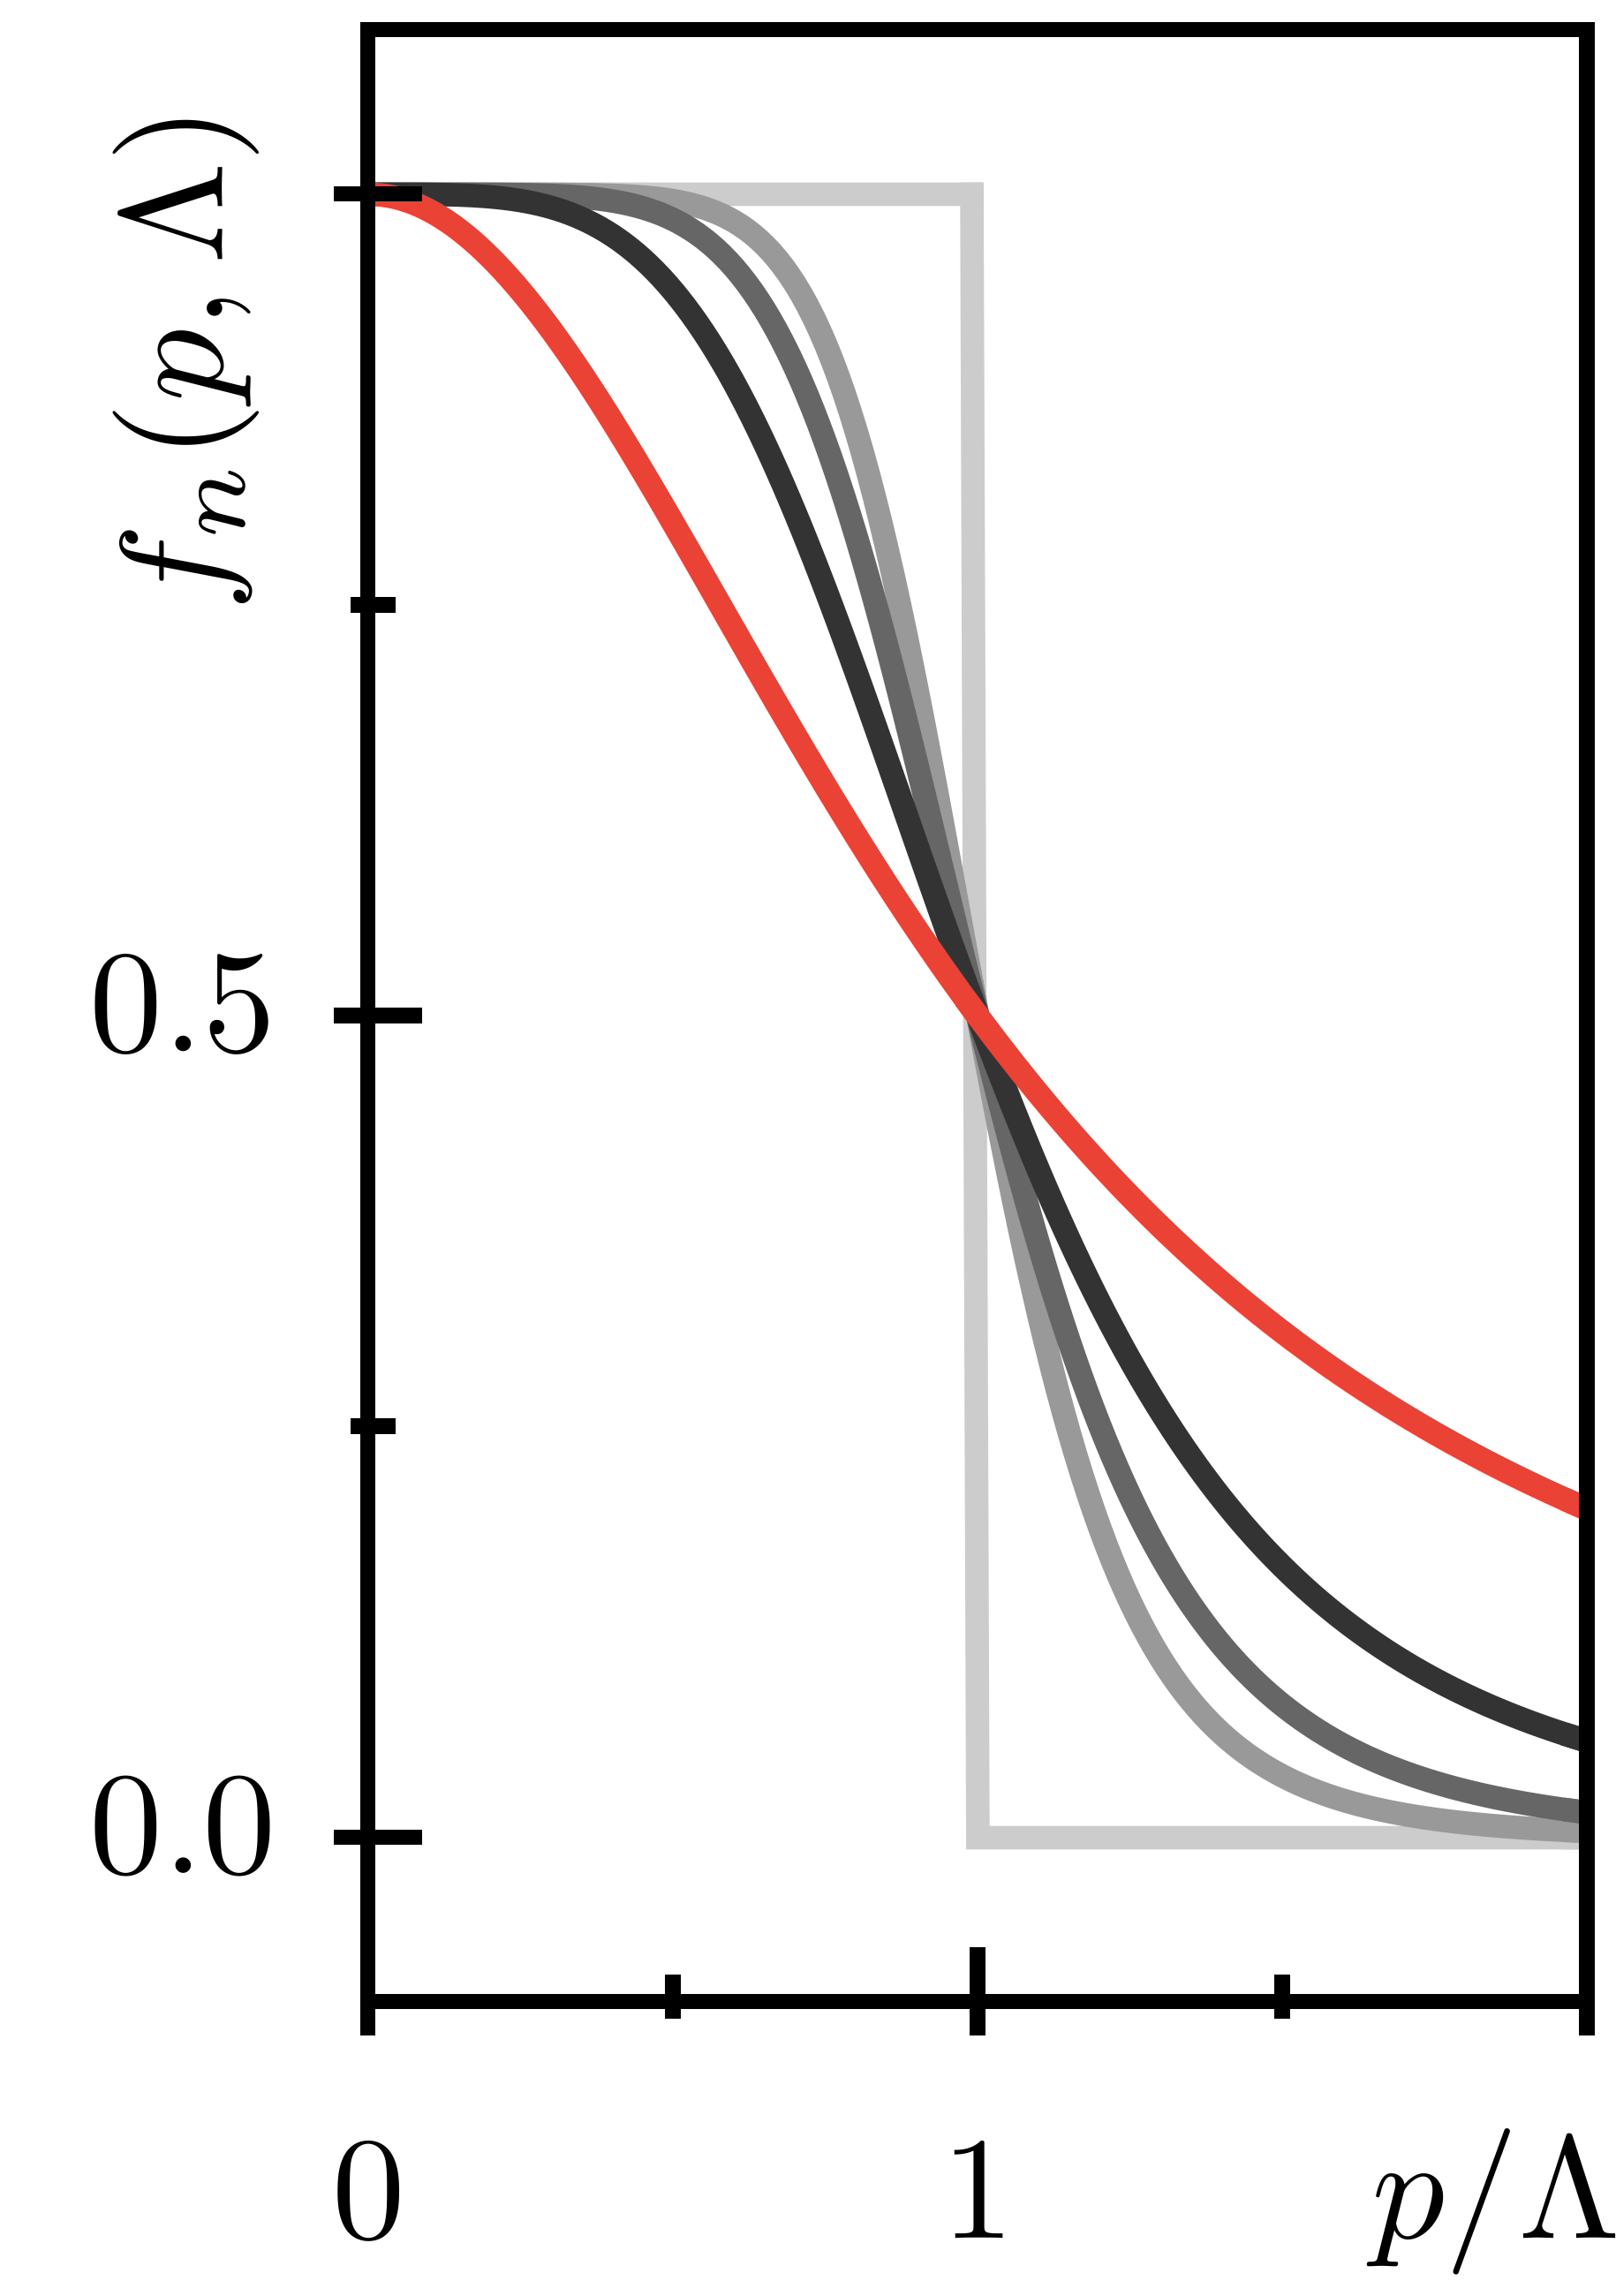
\includegraphics{figures/cutoff_function.png}}
    \subfigure[]{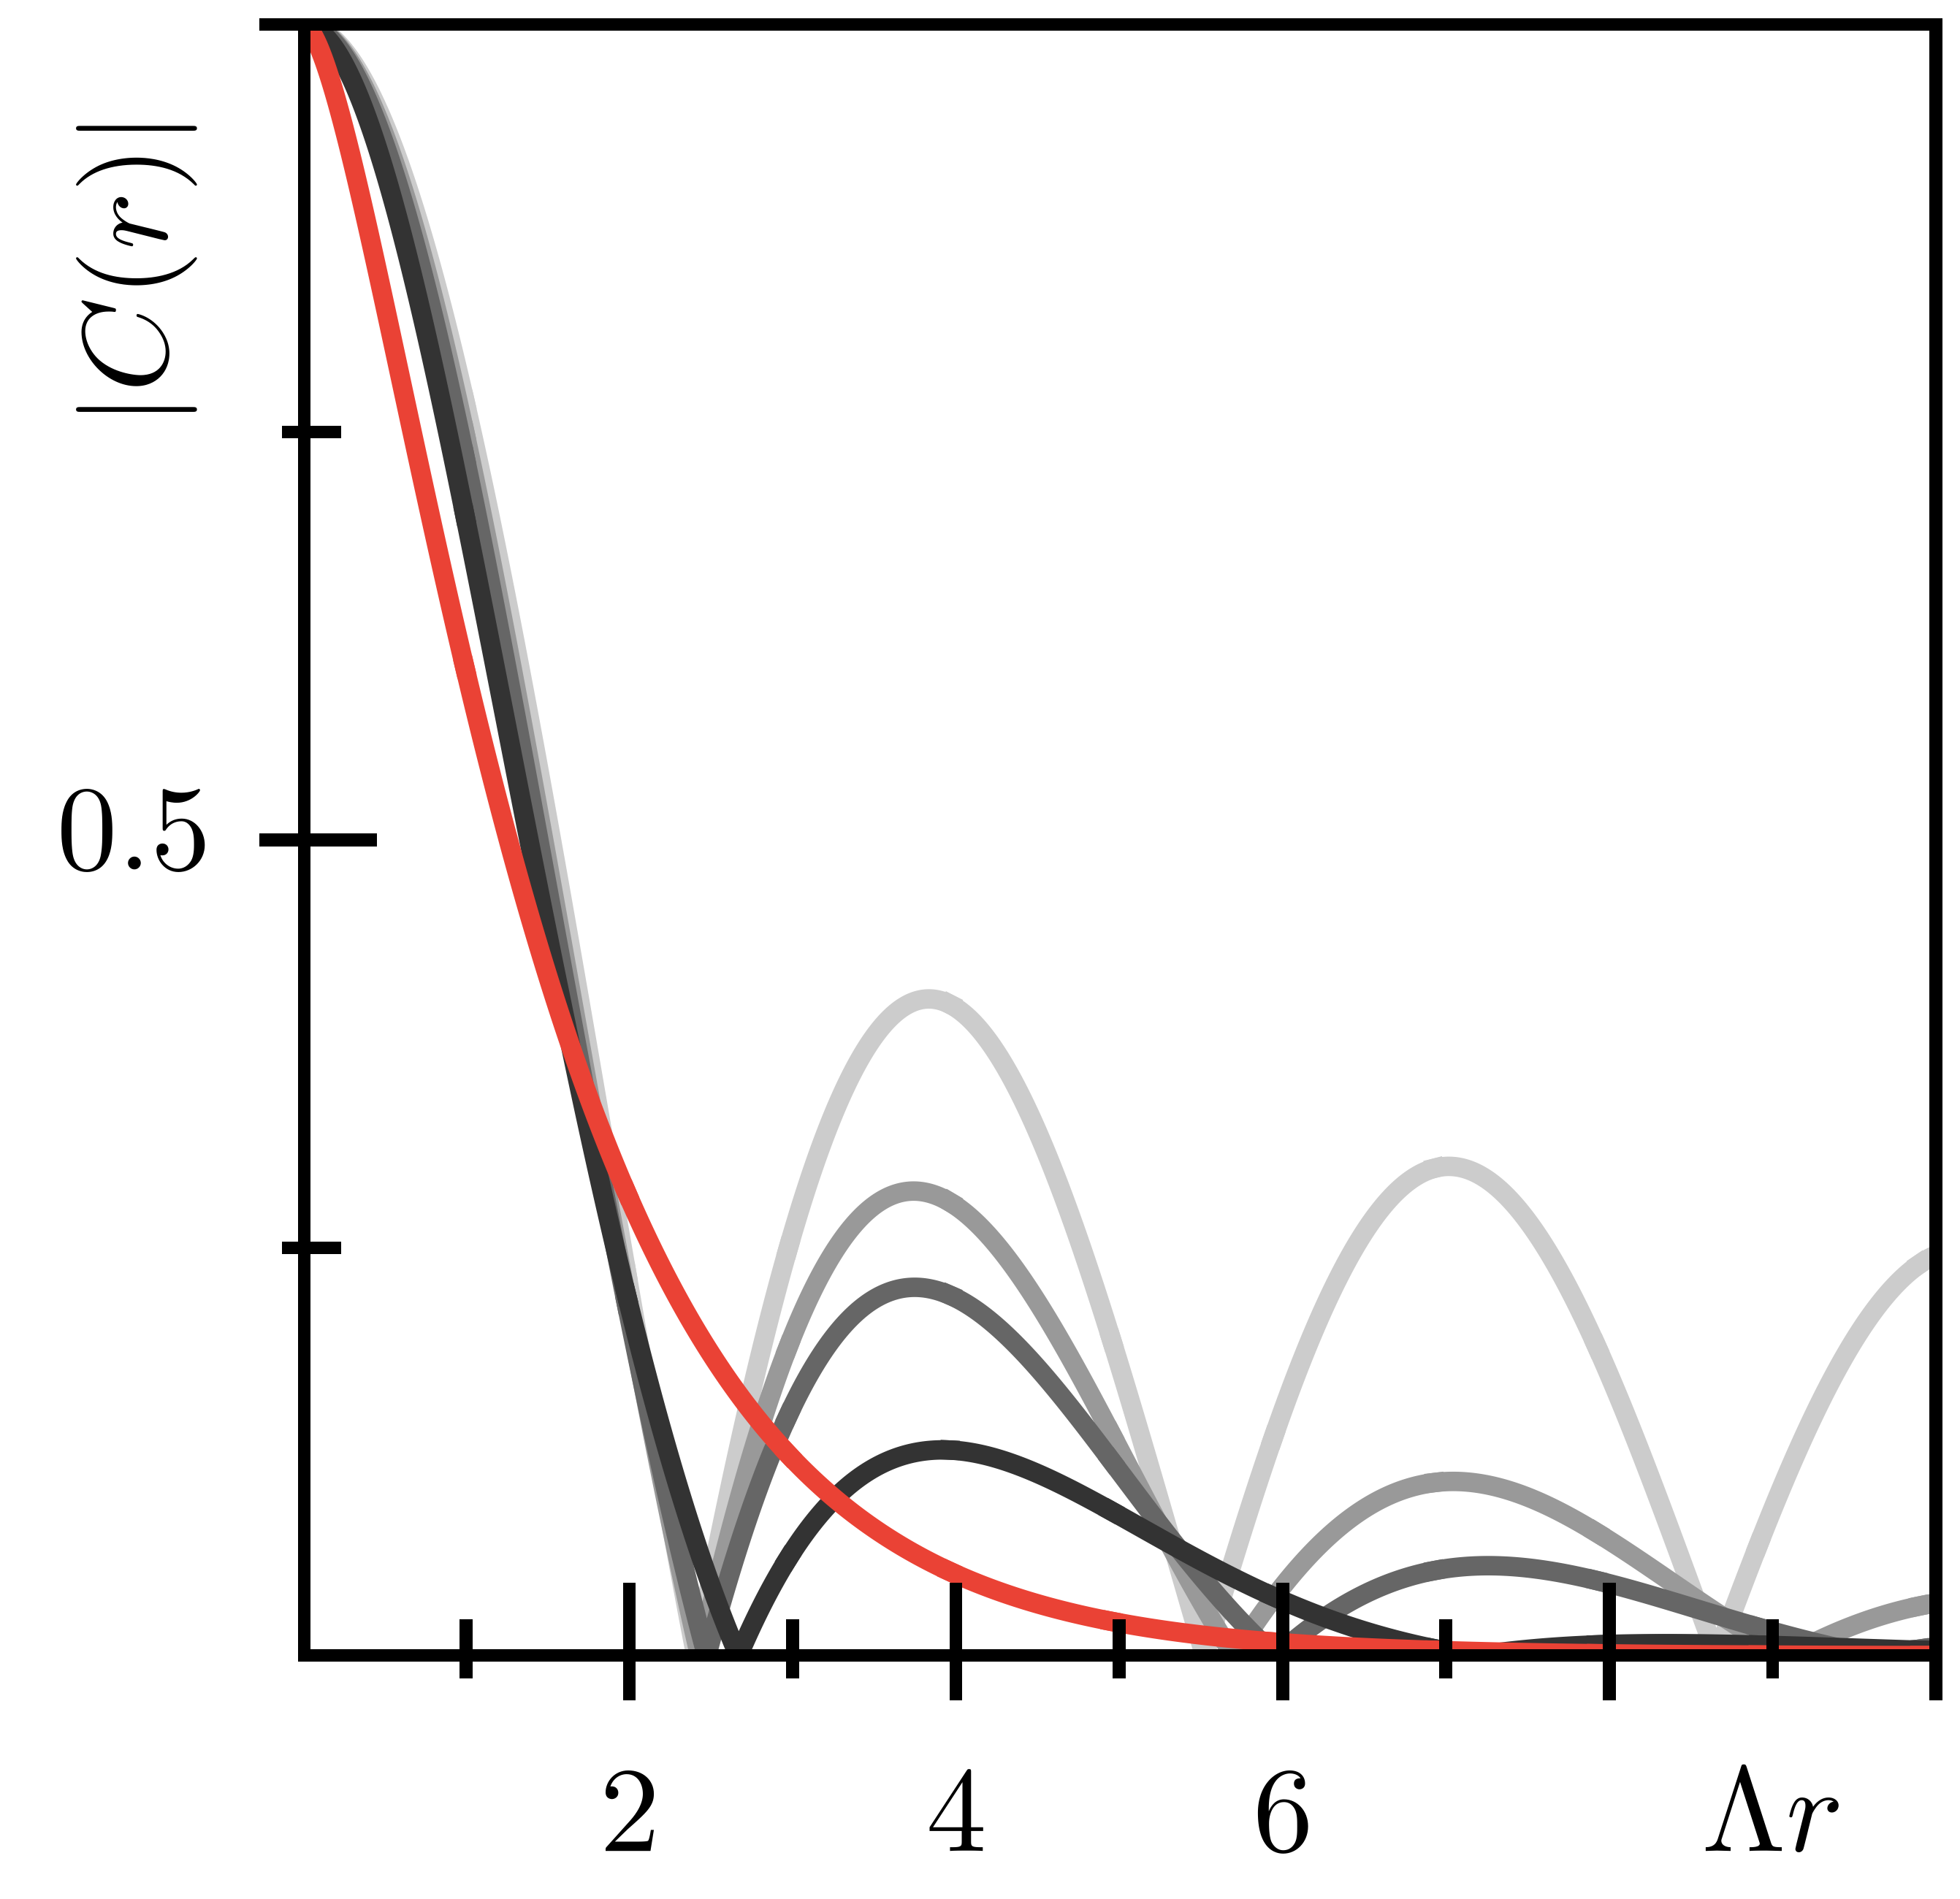
\includegraphics{figures/rg_correlations.png}}
    \subfigure[]{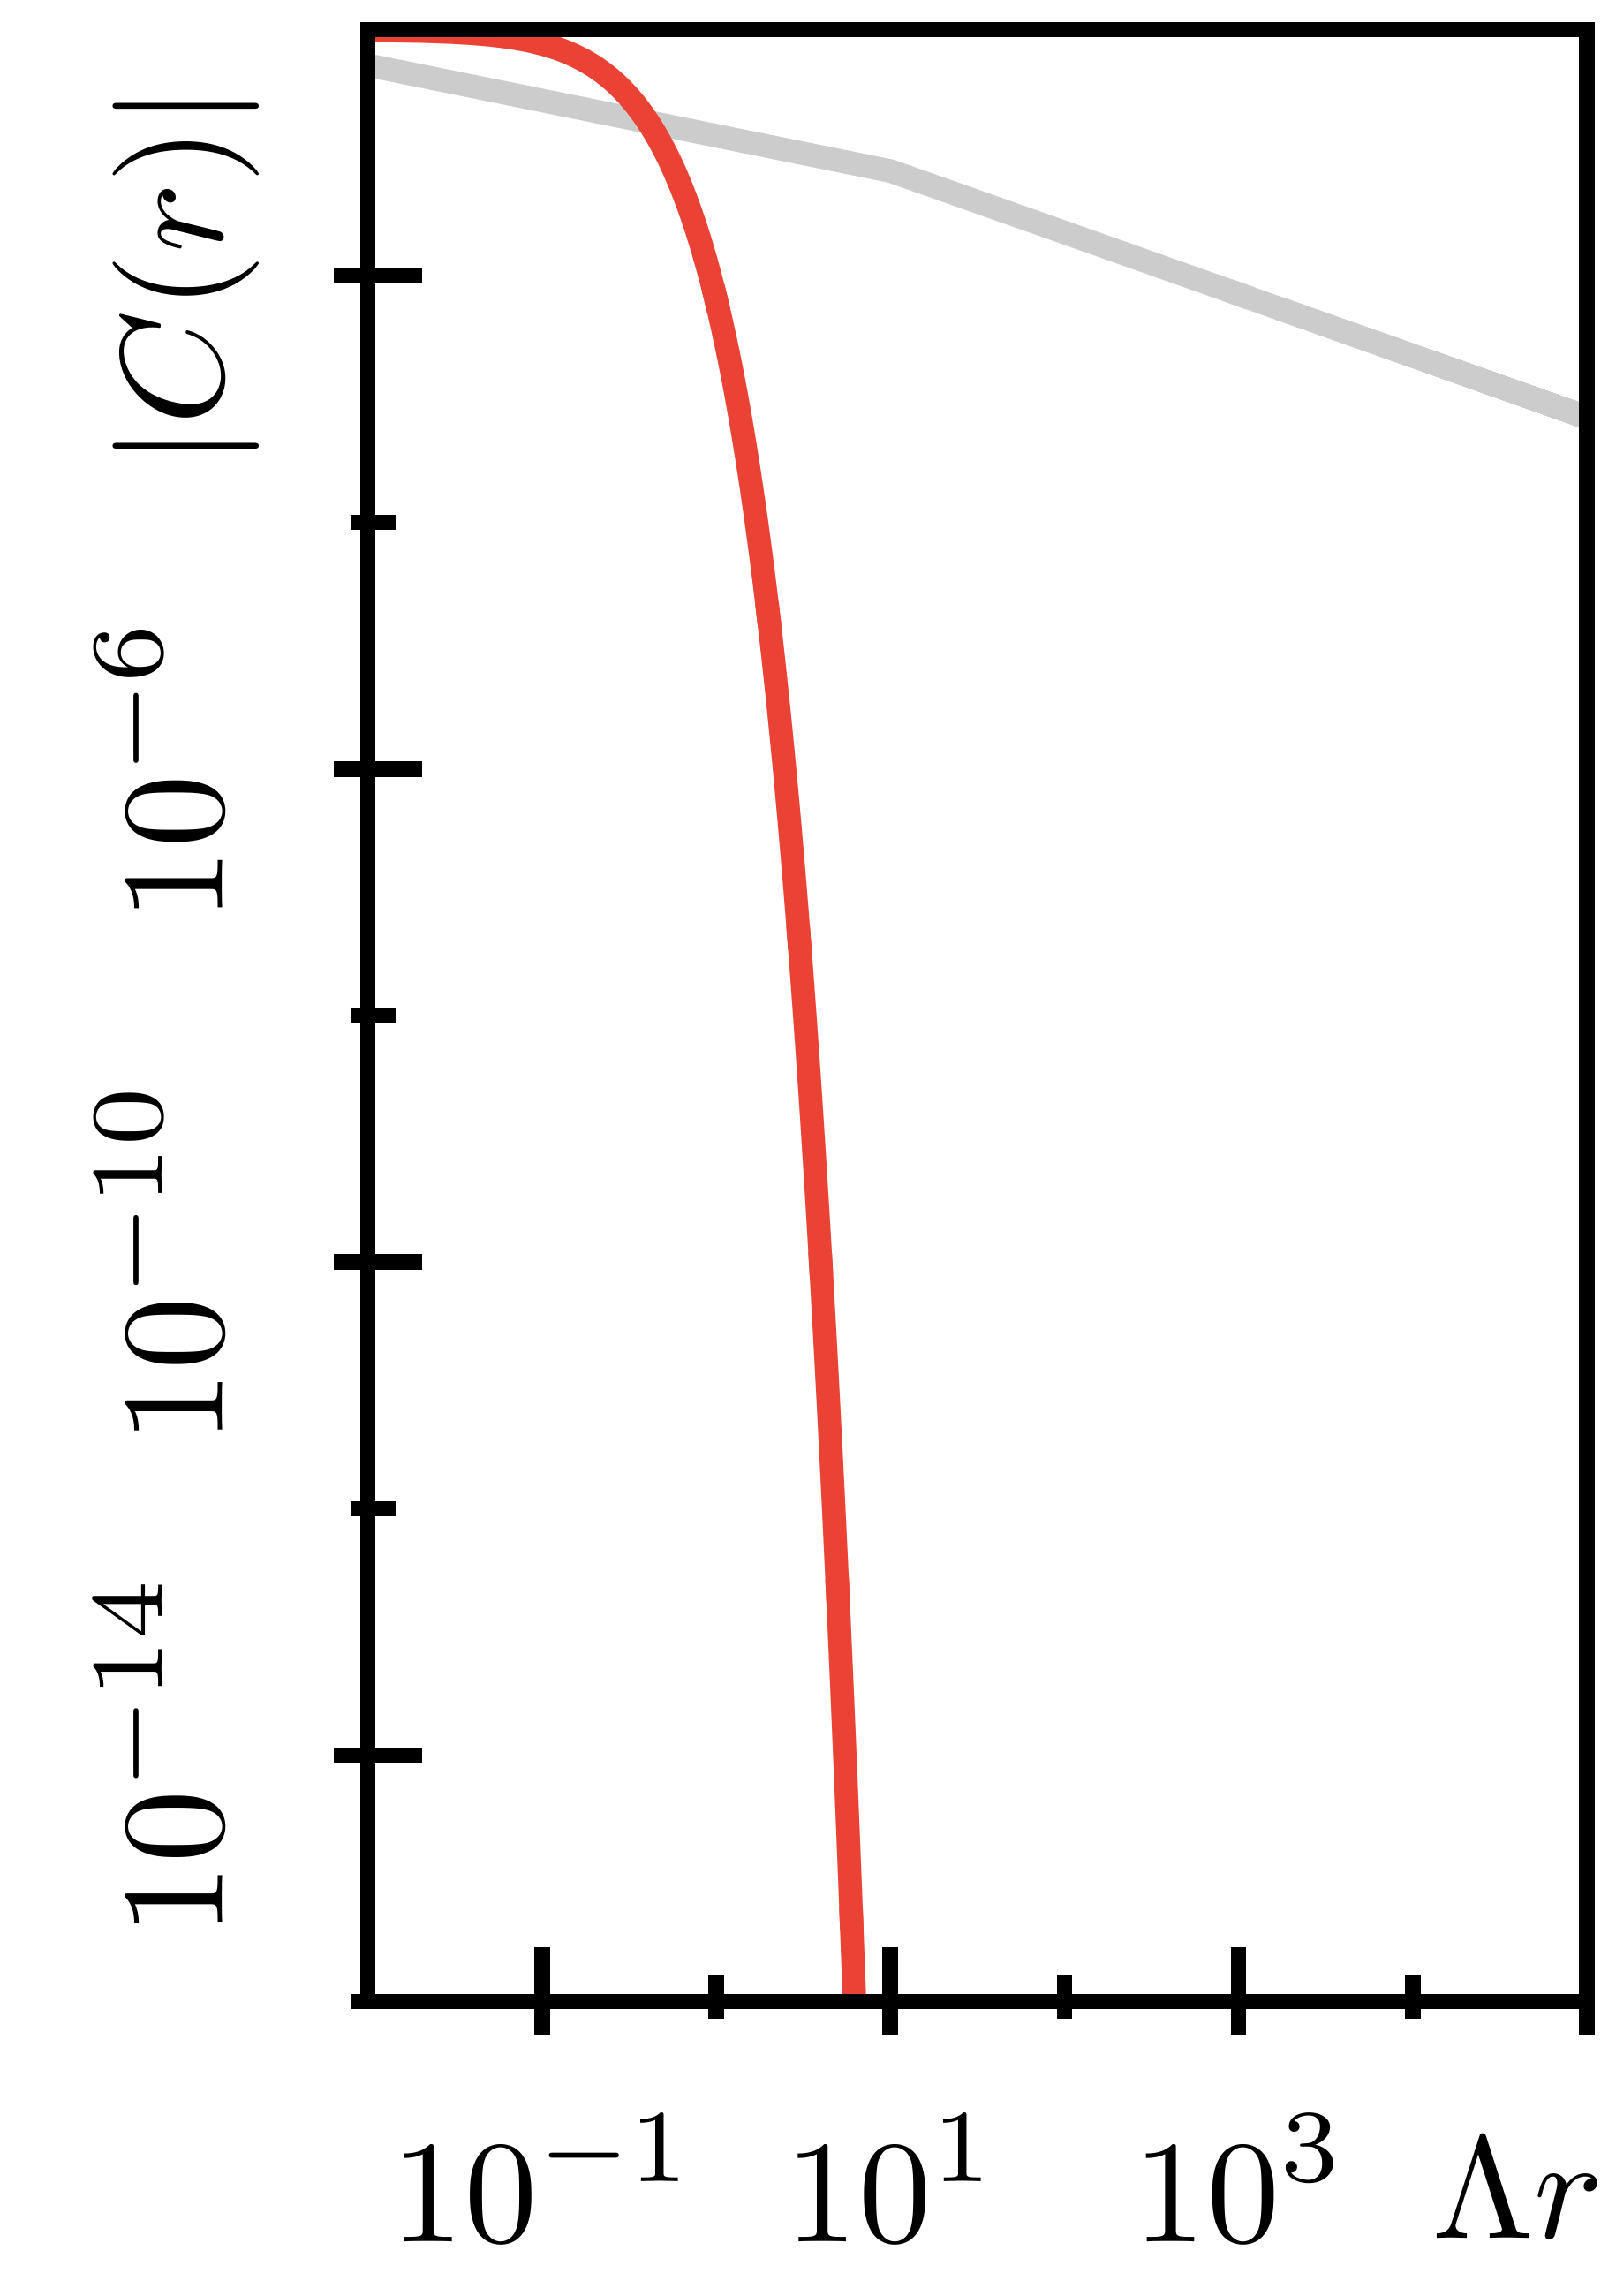
\includegraphics{figures/rg_correlations_log.png}}
    \caption{Panel (a) shows the chosen cutoff $f_n(p,\Lambda)$ with $n\in\{2,4,6,8,\infty\}$ for the integral expression in \cref{eq:integral_cutoff}, which results in various approximations of $C(r)$ for altering $n$ plotted in (b). Panel (c) highlights the exponentially sharp function $C_2(r)=\Lambda rK_1(r\Lambda)$ compared to the sharp cutoff result $C_\infty(r)=J_0(\Lambda r)$.}
    \label{fig:rg_cutoff}
\end{figure}
% At this point it is worth mentioning that the correlation functions of the slow fields are
% \begin{align}
%     \braket{\phi_\Lambda({\bf x}),\phi_\Lambda(\bf x')} = \frac K2\int_{0}^\infty\rd p J_0(p r)p^{n-1}\brlr{\frac1{p^n+\Lambda^n_{\rm min}}-\frac1{p^n+\Lambda^n_{\rm max}}}
% \end{align}
% which, in case of $n=2$, yield the appealing result
% \begin{align}
%     \braket{\phi_\Lambda({\bf x}),\phi_\Lambda(\bf x')} = \frac K2 \brlr{K_0(\Lambda_{\rm min} r) - K_0(\Lambda_{\rm max} r)}.
%     \label{eq:rg_slow_fields_approximation}
% \end{align}
For the special case $n=2$, the integral of the $h$-fields evaluates to $C_2(r)=\frac K2 \Lambda r K_1(\Lambda r)$ that decays exponentially fast (see \cref{fig:rg_cutoff}(c)).
In particular, the function follows the asymptotic decay $z K_1(z) \sim \sqrt{\pi z/2}\exp(-z)$ and is already negligible for $z=1$, i.e. $K_1(1)\approx0.0062$.
Therefore, the integration of $C_2(r)$ can be confined to a small interval $r<\xi$ in which $\xi\sim2\pi/\Lambda=a$ is a small length scale comparable with the lattice spacing $a$.
Without going into full detail, the smooth cutoff is the key ingredient to find the logarithmic expression of the propagator, with the general result
\begin{align}
    \int_{\Lambda_{\rm min}}^{\Lambda_{\rm max}}\rd p\frac{J_0(pr)}{2p}\rightarrow\int_{\Lambda_{\rm min}}^{\infty}\rd p\frac{J_0(pr)}{2p}f_n(p,\Lambda_{\rm max})\approx-\frac14\log\brlr{\frac{(\Lambda_{\rm max}^{-n}+r^n)^{\frac 2n}}{\Lambda_{\rm min}^{-2}}}.
\end{align}
In the above approximation, one first splits the integral into two parts, one ranging from the lower cutoff $\Lambda_{\rm min}$ to $1/r$, and the second from $1/r$ to infinity.
The asymptotic part of the integral decays algebraically as a function of $\Lambda_{\rm max}r$, it thus bears a small weight of the full integral and vanishes in the limit $\Lambda_{\rm max}\rightarrow\infty$.
The main weight of the integral resides in $[\Lambda_{\rm min},1/r]$, for which $J_0\approx1$ if the lower cutoff is chosen small enough.
This then yields the approximated propagator, with the special case $n=2$ used in~\cref{eq:kg_correlations_approximation}.

In order to utilize the confinement of $C_2$, it is beneficial to introduce relative coordinates ${\bf R} = 1/2({\bf x}+{\bf x'})$ and ${\bf r} = {\bf x}-{\bf x'}$.
The integral can then be rewritten to
\begin{align}
    -\frac12\braket{S^2_I[\phi_{\Lambda'}+h]}_{h,{\rm conn.}}
    =
    \frac{g^2K\beta^2}8\rd l\int\rd^2R\int\rd^2r
    C_2(r)
    \left(
        \cos\commutator{\beta\phi_{\Lambda'}({\bf R}+{\bf r})+\beta\phi_{\Lambda'}({\bf R}-{\bf r})}
        \right.
        \label{eq:rg_int_1}\\
        \left.-
        \cos\commutator{\beta\phi_{\Lambda'}({\bf R}+{\bf r})-\beta\phi_{\Lambda'}({\bf R}-{\bf r})}
    \right)
    \label{eq:rg_int_2}
    \\
    \approx
    \frac{g^2K\beta^2}{8}\rd l\int\rd^2R\rd^2rC_2(r)
    \left(
        \cos\commutator{2\beta\phi_{\Lambda'}({\bf R})}
        -
        \cos\commutator{\beta\partial_{\bf R}\phi_{\Lambda'}({\bf R}){\bf r})}
    \right).
    \label{eq:rg_int_rel_coords}
\end{align}
The $\cos$ term in \cref{eq:rg_int_1} did not exist in the original Hamiltonian -- it is a new sine-Gordon type interaction with higher scaling dimension $D_h = K\beta^2$.
Note that this term generation is continuous, and to account for it, we should start from a more generic interaction containing all the higher harmonics, i.e.
\begin{align}
    S_{I'} = S_I + \sum_{j=1}^\infty g_j\int\rd x\rd\tau\cos(2j\beta\phi).
    \label{eq:sine_gordon_full}
\end{align}
The first-order corrections of the Euclidian action then yield a coupled system of differential equations in which the amplitudes of less relevant operators depend on those of more relevant ones (but {\it not} vice-versa).
Note that this allows for a practical and well-justified simplification of dropping the sum in \cref{eq:sine_gordon_full}, because the dominant coupling is always independent of the amplitudes of less-relevant operators.

The $\cos$ term in (\cref{eq:rg_int_2}) yields a renormalization of the quadratic part after the harmonic approximation (neglecting the constant which renormalizes the free energy)
\begin{align}
    -\frac12\braket{S^2_I[\phi_{\Lambda'}+h]}_{h,{\rm conn.}}
    \approx
    \frac{\xi^4 g^2K\beta^4}{16u^2}\rd l\int\rd x\rd\tau\frac1{u^2}(\partial_
    \tau\phi_{\Lambda'})^2+(\partial_x\phi_{\Lambda'})^2.
    \label{eq:RG_second_order_approximation}
\end{align}
The constant $\xi^4/u^2$ is determined by the cutoff of the integrals over the relative coordinates, and $\xi\sim1/a$ is on the order of the lattice spacing.
In summary, we obtain the effective action
\begin{align}
    S_{\rm eff}^{(2)}[\phi_\Lambda] = \frac1{2\pi}\int\rd\brlr{ x\rd\tau\frac{1}{uK'}(\partial_\tau\phi_\Lambda)^2 + \frac{u}{K'}(\partial_x\phi_\Lambda)^2} +  g'\int\rd^2 x\cos(\beta\phi_\Lambda),
\end{align}
which is self-similar to the original action up to the renormalized couplings
\begin{align}
    \frac1{uK'}=\frac1{uK}+\frac{\xi^4 g^2 K\beta^4\pi}{8 u^4}\rd l,
    \quad
    \frac u{K'}=\frac u{K}+\frac{\xi^4 g^2 K\beta^4\pi}{8u^2}\rd l,
    \quad
    g' = g\brlr{1 + \commutator{2-\frac{\beta^2 K}4}\rd l},
    \\
    \Rightarrow
    K' = \brlr{\commutator{\frac{1}{uK}+\frac{\xi^4 g K\beta^4\pi}{8u^4}}\commutator{\frac{u}{K}+\frac{\xi^4 g K\beta^4\pi}{8u^2}}}^{-1/2}
    =
    K-\frac{\pi \xi^4 \beta^4 g^2 K^3}{8u^2}\rd l + O(\rd l^2).
\end{align}
In summary, this concludes the derivation of the so-called RG flow which is described by the system of differential equations we just derived
\begin{align}
    \frac{\rd K}{\rd l} = -\frac{\pi \xi^4 \beta^4 g^2 K^3}{8u^2},
    \quad
    \frac{\rd g}{\rd l} = g\brlr{2-\frac{\beta^2K}4}.
\end{align}
Viable estimates are already obtained far from the phase transitions, and the second order approximation provides more insights close to the phase transition at $D_g=2$, in particular at $K=8/\beta^2$.
Equivalent results are obtained for the dual field by replacing $K\rightarrow K^{-1}$.
It is beneficial to define the flow equations close to the critical point, e.g. through the parameters
\begin{align}
    x = \frac{\beta^2 K}4 - 2,
    \quad
    y = 4g\sqrt{\frac{\pi\xi^4}{u^2}},
\end{align}
which dictate the modified RG equations
\begin{align}
    \frac{\rd x}{\rd l} = -\frac{y^2}8(x+2)^3,
    \quad
    \frac{\rd y}{\rd l} = - xy.
\end{align}
These equations can be depicted as stream lines in the $x,y$ plane, as depicted in \cref{fig:bkt_flow_equations}.
Note that $x$ represents the effective Luttinger parameter and $y$ an effective coupling of the sine-Gordon interaction.
In particular, we obtain four scenarios.
(i) If $x>0$, and $y<x$, the system flows towards $y=0$ and a finite value of $x$ upon which the flow ends.
This is a situation in which the interaction is irrelevant and the coupling vanishes.
Note that although the interaction is irrelevant and as such the system remains in a Luttinger liquid phase, it ``renormalizes'' the effective Luttinger liquid parameter during the flow.
(ii) If $x>0$ and $y=x$ (taken in proximity of $x$ and $y$ small), the trajectory follows a critical BKT line to the fix point $x=y=0$.
(iii) In case of $y>x$, the coupling flows towards infinite, independently on value of $x$.
This corresponds to a case in which the interaction becomes dominating.
The Luttinger liquid description breaks down and the system ends up in a gapped phase, characterized by the interaction.
(iv) For $x<0$, the system flows towards $y\rightarrow\infty$, which is also a gapped phase.
In this case, the initial value of $y$ does not matter and even a perturbative interaction will result in the formation of a gap.
This is the ``relevant'' case, since the dominance of $y$ is determined by the initial value of $x$, and even a perturbatively small interaction amplitude results in the breakdown of the Luttinger liquid description and the formation of an energy gap.

\begin{figure}
    \centering
    \subfigure[]{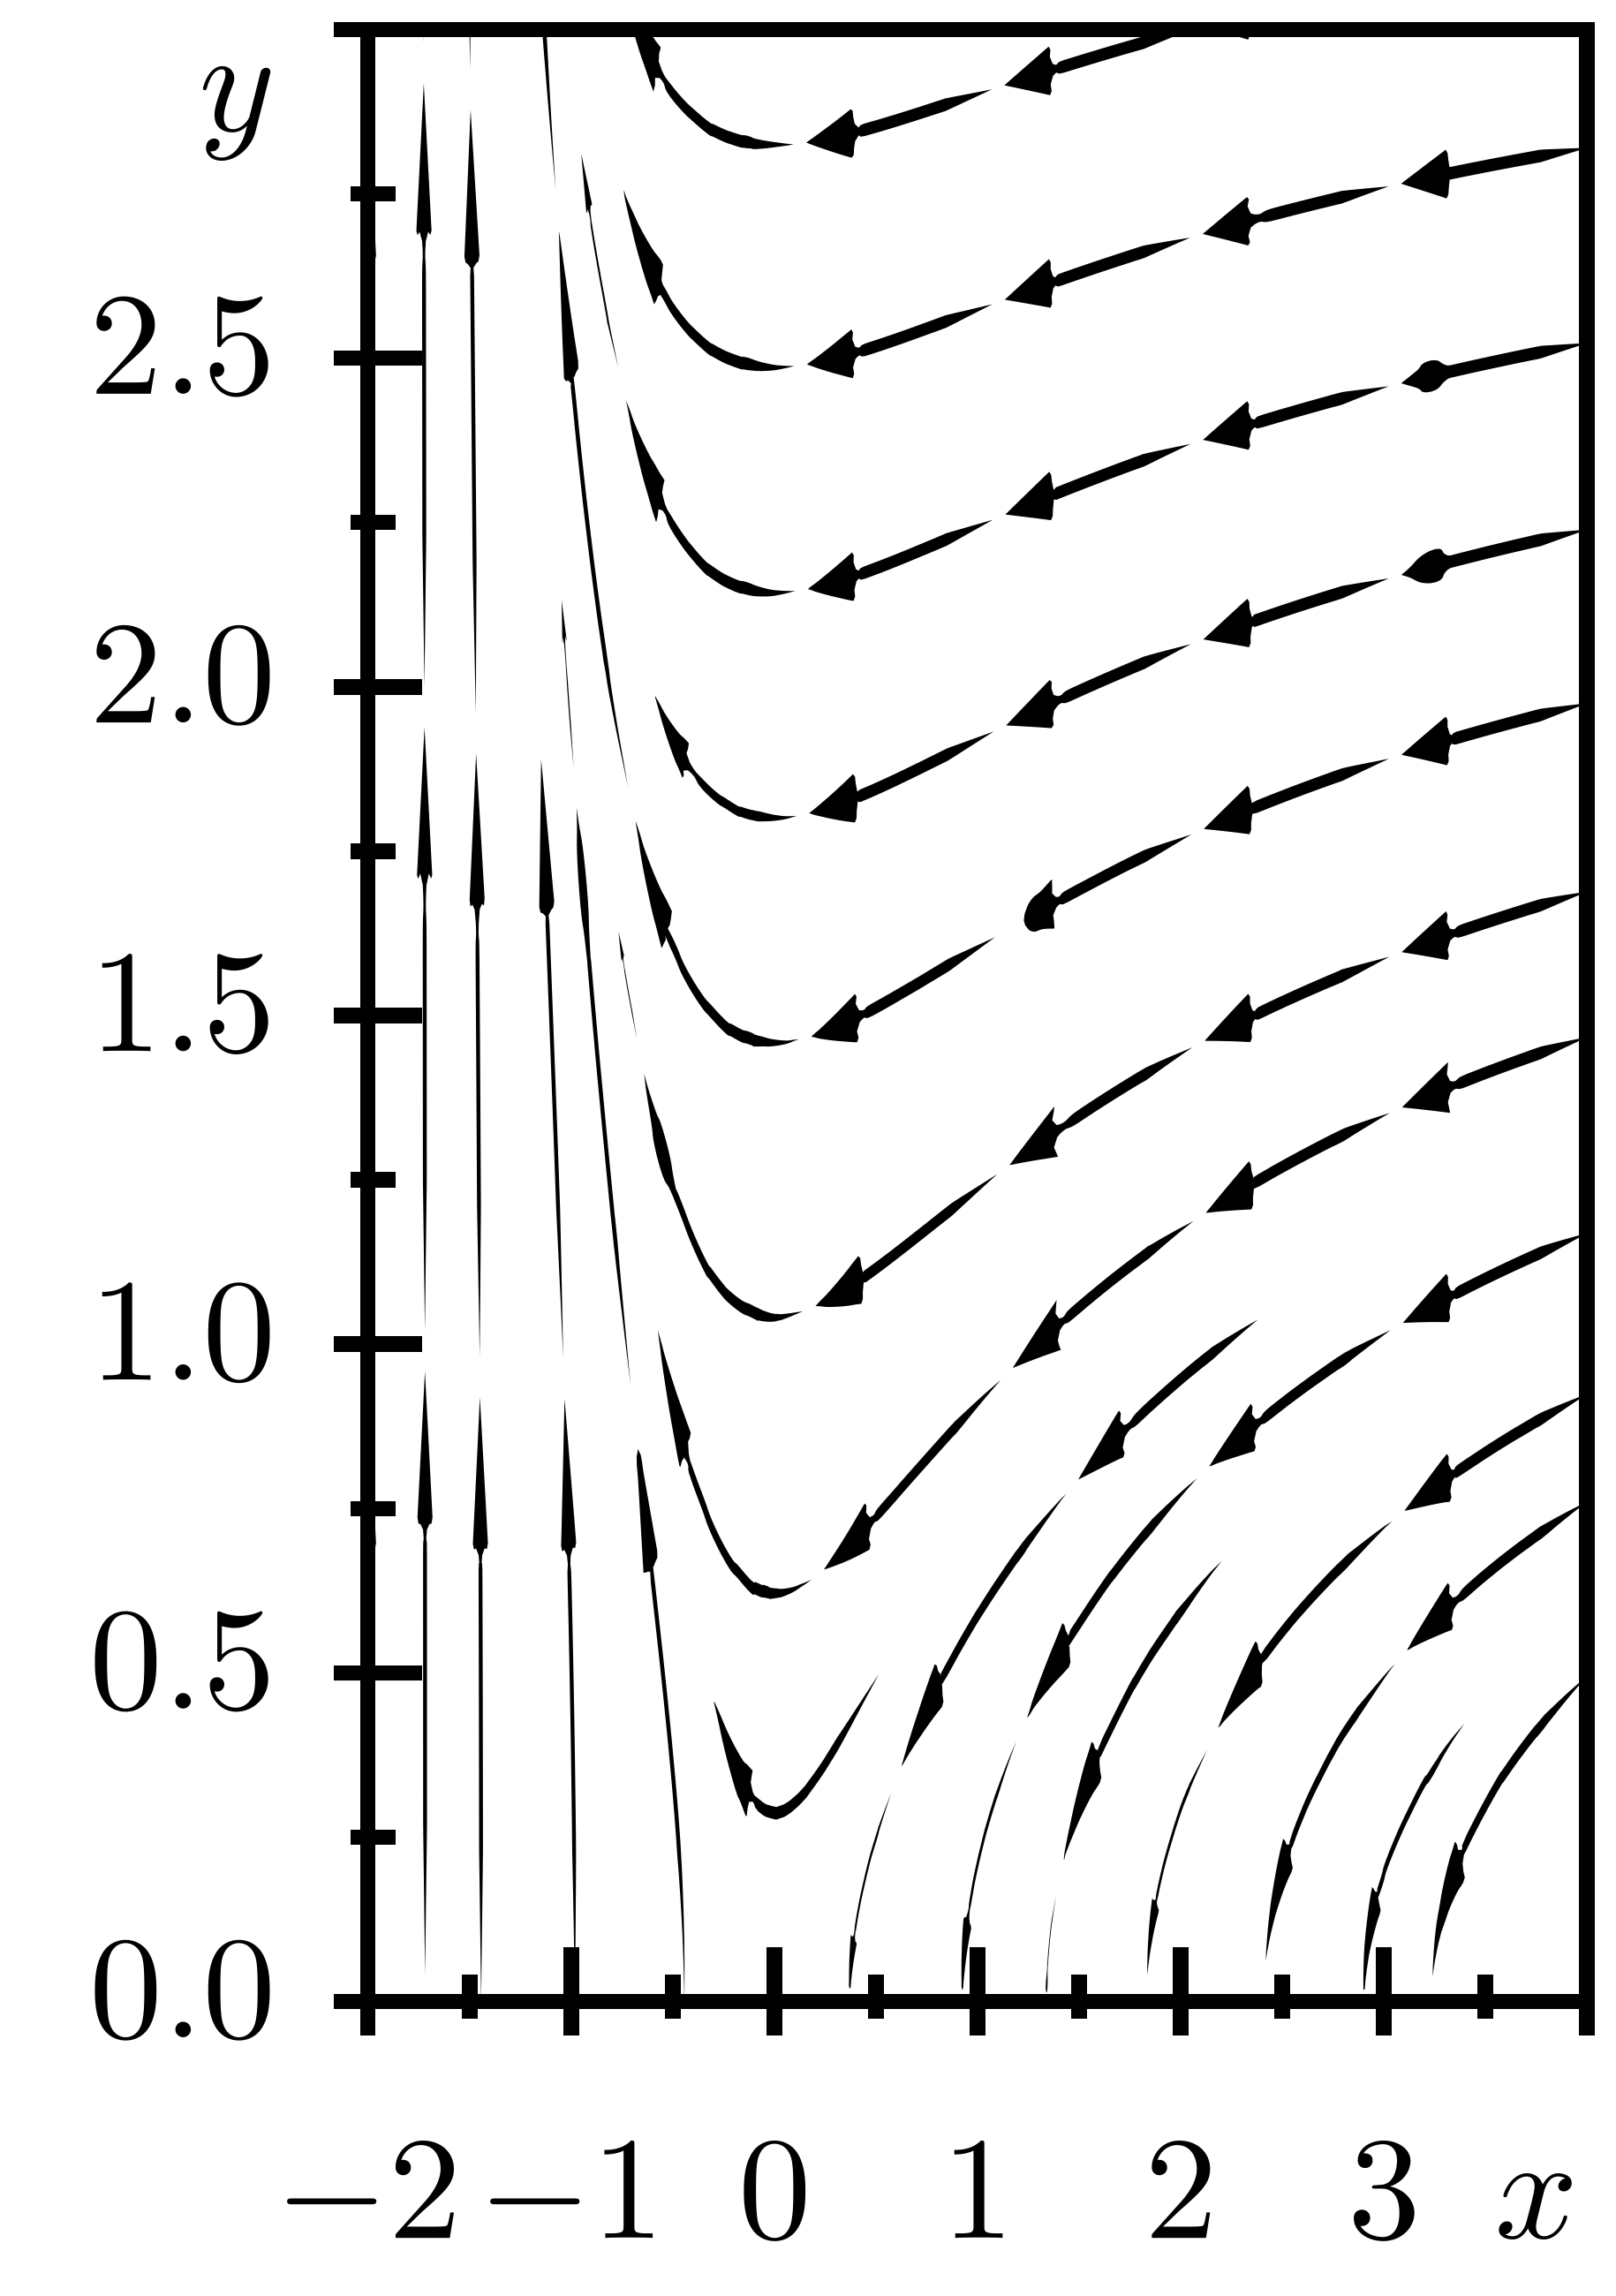
\includegraphics{figures/BKT_RG_flow1.png}}
    \subfigure[]{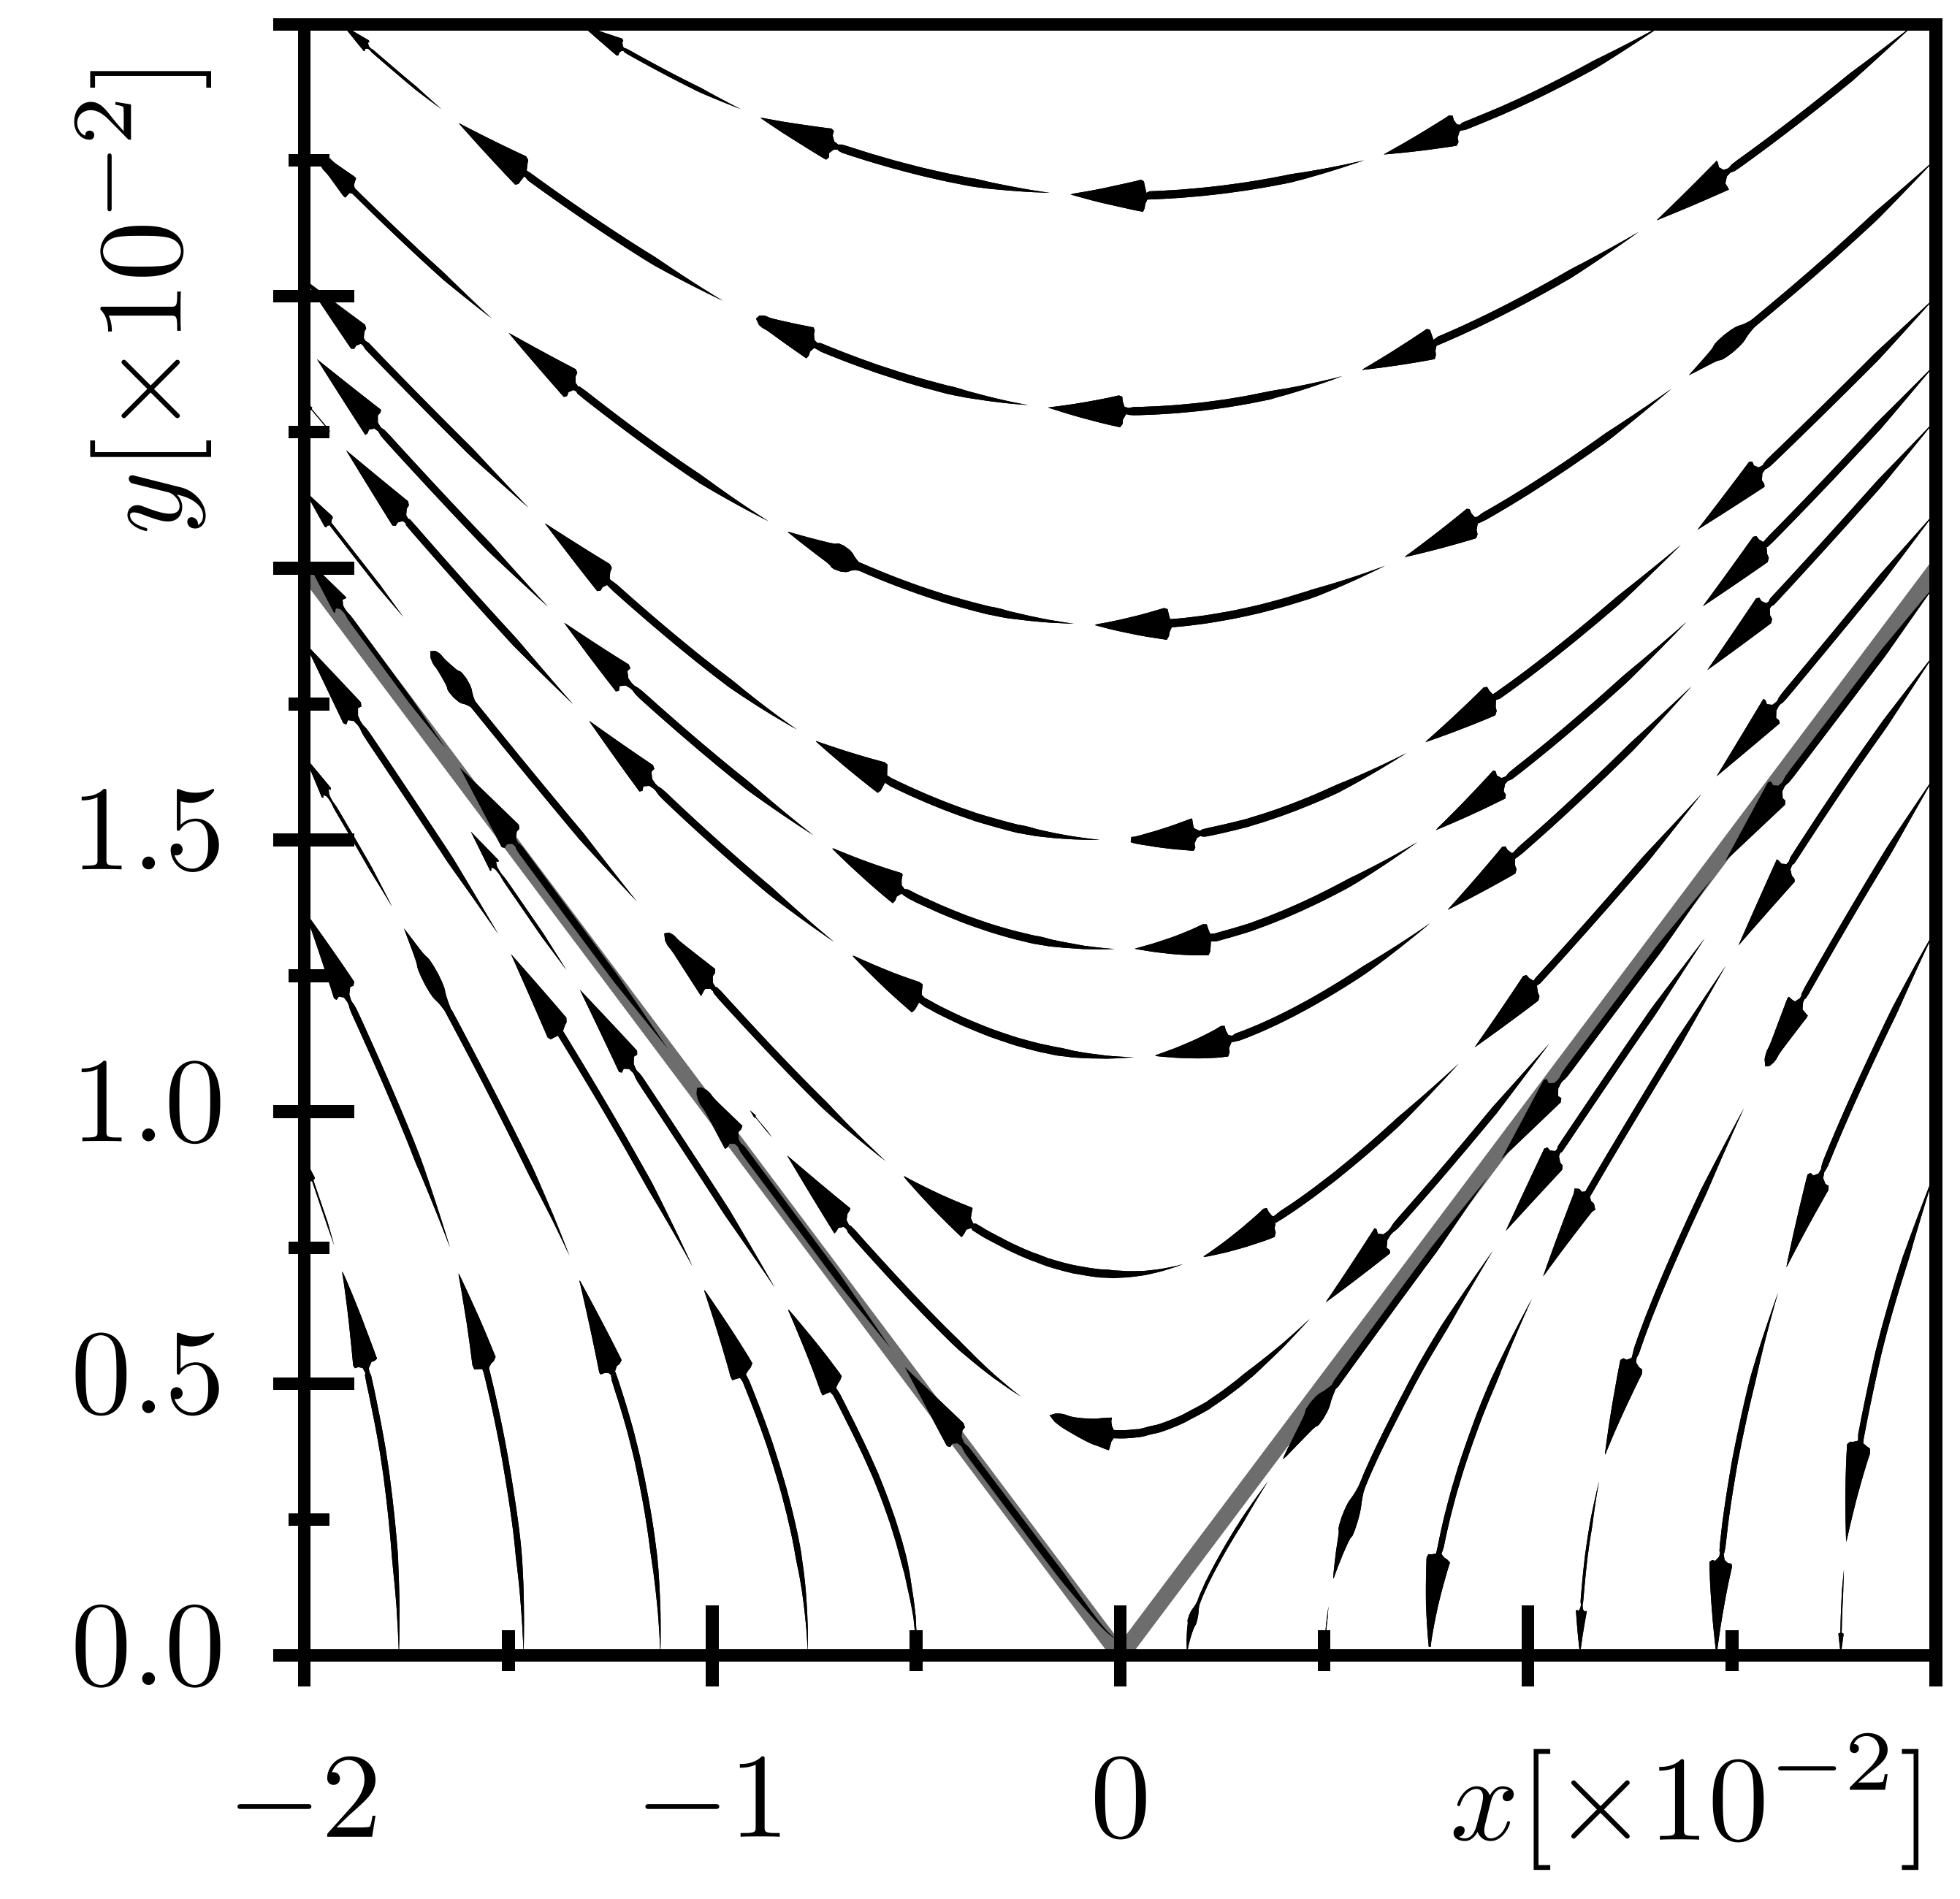
\includegraphics{figures/BKT_RG_flow2.png}}
    \subfigure[]{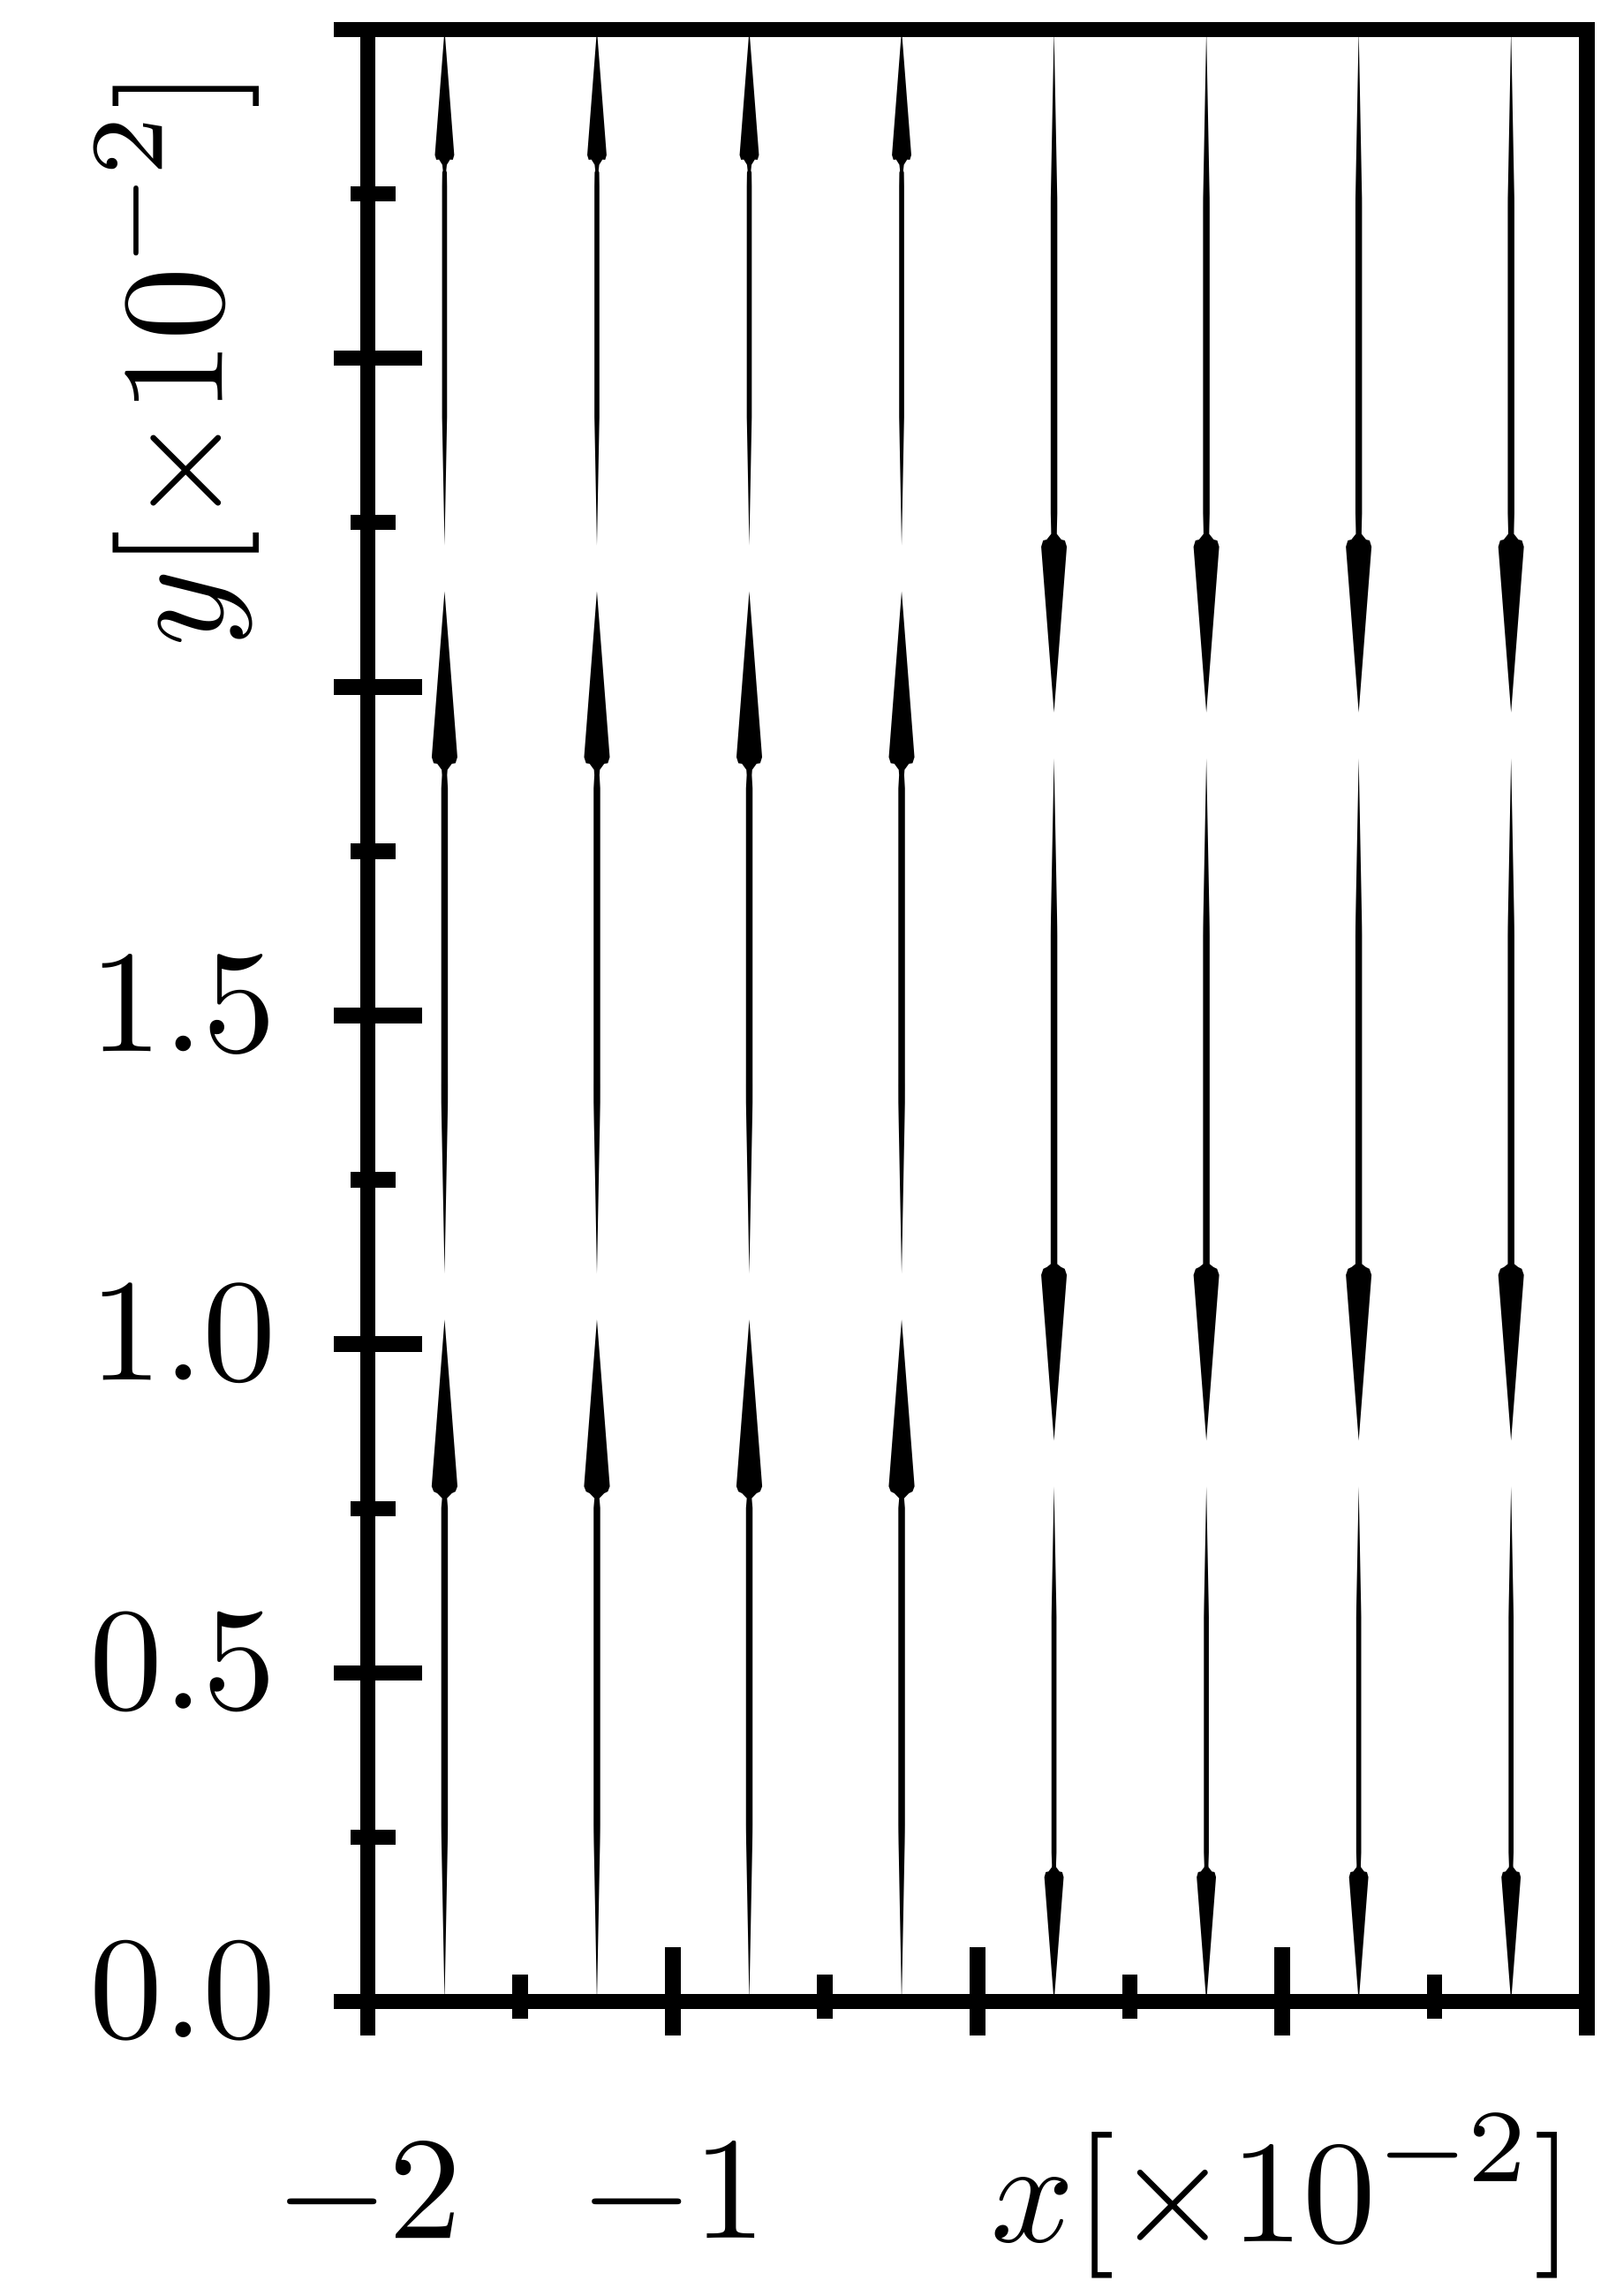
\includegraphics{figures/BKT_RG_flow3.png}}
    \caption{Plot of the modified RG equations far (a) and close (b) to the critical point $x=0$. Panel (b) close to the transition at $x=0$ shows four different scenarios for $g>0$: (i) $x>0$ and $y<x$ drives the coupling $y\rightarrow0$. This is the regime in which $g$ is irrelevant such that the system remains in the Luttinger liquid phase. (ii) $x>0$ and $y=x$ describes the critical BKT line which flows to the critical fix point $x=y=0$. (iii) $y>x$, the system always flows to $y\rightarrow\infty$ independently of $x$. (iv) $x<0$, the system flows to $y\rightarrow\infty$. Panel (c) contrasts the results of the first order RG approximation which neglects the flow of the Luttinger parameter $K$.}
    \label{fig:bkt_flow_equations}
\end{figure}

\todo{Reference to the research}
